% main.tex
\documentclass[a4paper,11pt,color]{report}
% -----------------------------
% Basic document setup (load first)
% -----------------------------
\usepackage[a4paper]{geometry}  % Page layout settings
\usepackage[german,english]{babel}  % Language support
\usepackage{csquotes}  % Required by babel/biblatex

% -----------------------------
% Font and encoding packages
% -----------------------------
\usepackage{fontspec}  % XeLaTeX font support
\usepackage{textcomp}  % Additional symbols
\usepackage{gensymb}  % General symbols
%\usepackage{FiraSans}
%\usepackage{tgpagella}
%\usepackage{tgbonum}
%\usepackage{libertine}

% -----------------------------
% Math packages
% -----------------------------
\usepackage{amsmath}
\usepackage{amssymb}
%\usepackage{amsthm}
\usepackage{amsfonts}
\usepackage{esvect}
\usepackage{commath}
\usepackage{tcolorbox}

% -----------------------------
% Graphics and color
% -----------------------------
\usepackage{graphicx}  % Image support
\usepackage{xcolor}    % Color support (includes color package functionality)
\usepackage{subfigure}
\usepackage{tikz}
\usepackage{pgf-umlcd}
\usepackage{float}
\usepackage{pdfpages}

% -----------------------------
% Plots
% -----------------------------

\usepackage{pgfplots}
\usepackage{pgfplotstable}
\pgfplotsset{compat=newest}

% -----------------------------
% Lists and algorithms
% -----------------------------
\usepackage{enumerate}
%\usepackage[plain,chapter]{algorithm}
\usepackage{algorithmic}
\usepackage{listings}
\usepackage{booktabs}

% -----------------------------
% Theorem environments
% -----------------------------
\usepackage[amsmath,thmmarks]{ntheorem}

% -----------------------------
% Typography improvements
% -----------------------------
\usepackage{microtype}  % Better typography
\usepackage{sectsty}    % Section title formatting

% -----------------------------
% Formatting
% -----------------------------
\usepackage{seqsplit}

% -----------------------------
% Captions and URLs
% -----------------------------
\usepackage[margin=0pt,font=small,labelfont=bf]{caption}
\usepackage{url}

% -----------------------------
% Bibliography setup (load late)
% -----------------------------
\usepackage[backend=biber,
    style=numeric,      % numbered citations
    sorting=none,       % numbers appear in citation order
    urldate=long,       % includes date when website was accessed
    hyperref=true]{biblatex}
\addbibresource{literatur/diplom.bib}

% -----------------------------
% Load hyperref last
% -----------------------------

\usepackage[hidelinks]{hyperref}

% -----------------------------
% Package-specific settings
% -----------------------------

% set default fonts
\setmainfont{Linux Libertine O}

% dont write CHAPTER at the beginning of every chapter. Just the number and chapter title.
\makeatletter
\def\@makechapterhead#1{%
    \vspace*{50\p@}%
    {\parindent \z@ \raggedright
        \ifnum \c@secnumdepth >\m@ne
            \huge\bfseries \thechapter\space\space%
        \fi
        \interlinepenalty\@M
        \huge \bfseries #1\par\nobreak
        \vskip 40\p@
    }}
\makeatother

% Change sizes for different heading levels
%\chapterfont{\huge}          % For chapters
\sectionfont{\Large}         % For sections
\subsectionfont{\large}      % For subsections
\subsubsectionfont{\normalsize}  % For subsubsections

\lstset{
    frame=none,
    breaklines=true,
    basicstyle=\ttfamily\footnotesize,
    keywordstyle=\color{blue},
    commentstyle=\color{green!60!black},
    stringstyle=\color{red},
    numbers=left,
    numberstyle=\tiny
    %numbersep=5pt
}

\newlength{\widefigwidth}
\setlength{\widefigwidth}{\paperwidth}
\addtolength{\widefigwidth}{-4cm}

% -----------------------------
% Set theorem styles
% -----------------------------
% Define the theorem styles
% \theoremstyle{definition}  % Style for examples (upright font)
% \newtheorem{example}{Example}[section]

% \theoremstyle{remark}     % Style for remarks (upright font, no special formatting)
% \newtheorem{remark}{Remark}[section]

% Define the theorem styles
\tcbuselibrary{theorems}
\tcbuselibrary{skins}  % For enhanced style
\tcbuselibrary{breakable}  % For allowing page breaks
\tcbuselibrary{listings}  % For code formatting
\newtcbtheorem[number within=chapter]{example}{Example}{
    enhanced,
    colback=white,
    colframe=black!50,
    fonttitle=\bfseries,
    colbacktitle=white,
    coltitle=black,
    attach boxed title to top left={yshift=-2mm, xshift=2mm},
    boxed title style={
            size=small,
            colframe=white,
            colback=white
        },
    before upper={\parindent15pt}
}{ex}

\newtcbtheorem[number within=chapter]{remark}{Remark}{
    enhanced,
    colback=gray!5,
    colframe=gray!50,
    fonttitle=\bfseries,
    colbacktitle=gray!5,
    coltitle=black,
    attach boxed title to top left={yshift=-2mm, xshift=2mm},
    boxed title style={
            size=small,
            colframe=gray!5,
            colback=gray!5
        },
    before upper={\parindent15pt}
}{rem}

% Define the algorithm style with listing support
\newtcbtheorem[number within=section]{algorithm}{Algorithm}{
  enhanced,
  colback=white,
  colframe=black!50,
  fonttitle=\bfseries,
  colbacktitle=white,
  coltitle=black,
  left=2mm,          % Added for internal margin control
  right=2mm,         % Added for internal margin control
  top=0mm,           % Added for internal margin control
  bottom=0mm,        % Added for internal margin control
  before skip=3pt,   % Added for external margin control
  after skip=3pt,    % Added for external margin control
  attach boxed title to top left={yshift=-2mm, xshift=2mm},
  boxed title style={
    size=small,
    colframe=white,
    colback=white
  },
  listing engine=listings,  % Specify listing engine
  listing only,            % Important!
  listing options={
    language=C++,       % Specify the language
    numbers=left,
    numberstyle=\tiny,
    basicstyle=\ttfamily\small,
    keywordstyle=\color{blue}\bfseries,
    commentstyle=\color{green!60!black},
    showstringspaces=false,
    breaklines=true,
    postbreak=\mbox{\textcolor{red}{$\hookrightarrow$}\space},
  },
  breakable=false,
  before upper={\parindent15pt}
}{alg}

\makeatletter
\newcommand\tcb@cnt@algorithmautorefname{Algorithm}
\makeatother
% change headings to sans serif
% \chapterfont{\selectfont}
% \allsectionsfont{\sffamily}

% % Theorem-Optionen %
% \theoremseparator{.}
% \theoremstyle{change}
% \newtheorem{theorem}{Theorem}[section]
% \newtheorem{satz}[theorem]{Satz}
% \newtheorem{lemma}[theorem]{Lemma}
% \newtheorem{korollar}[theorem]{Korollar}
% \newtheorem{proposition}[theorem]{Proposition}
% % Ohne Numerierung
% \theoremstyle{nonumberplain}
% \renewtheorem{theorem*}{Theorem}
% \renewtheorem{satz*}{Satz}
% \renewtheorem{lemma*}{Lemma}
% \renewtheorem{korollar*}{Korollar}
% \renewtheorem{proposition*}{Proposition}
% % Definitionen mit \upshape
% \theorembodyfont{\upshape}
% \theoremstyle{change}
% \newtheorem{definition}[theorem]{Definition}
% \theoremstyle{nonumberplain}
% \renewtheorem{definition*}{Definition}
% % Kursive Schrift
% \theoremheaderfont{\itshape}
% \newtheorem{notation}{Notation}
% \newtheorem{konvention}{Konvention}
% \newtheorem{bezeichnung}{Bezeichnung}
% \theoremsymbol{\ensuremath{\Box}}
% \newtheorem{beweis}{Beweis}
% \theoremsymbol{}
% \theoremstyle{change}
% \theoremheaderfont{\bfseries}
% \newtheorem{bemerkung}[theorem]{Bemerkung}
% \newtheorem{beobachtung}[theorem]{Beobachtung}
% \newtheorem{beispiel}[theorem]{Beispiel}
% \newtheorem{problem}{Problem}
% \theoremstyle{nonumberplain}
% \renewtheorem{bemerkung*}{Bemerkung}
% \renewtheorem{beispiel*}{Beispiel}
% \renewtheorem{problem*}{Problem}

% % Algorithmen anpassen %
% \renewcommand{\algorithmicrequire}{\textit{Eingabe:}}
% \renewcommand{\algorithmicensure}{\textit{Ausgabe:}}
% \floatname{algorithm}{Algorithmus}
% \renewcommand{\listalgorithmname}{Algorithmenverzeichnis}
% \renewcommand{\algorithmiccomment}[1]{\color{grau}{// #1}}

% % Zeilenabstand einstellen %
% \renewcommand{\baselinestretch}{1.25}
% % Floating-Umgebungen anpassen %
% \renewcommand{\topfraction}{0.9}
% \renewcommand{\bottomfraction}{0.8}
% % Abkuerzungen richtig formatieren %
% \usepackage{xspace}
% \newcommand{\vgl}{vgl.\@\xspace}
% \newcommand{\zB}{z.\nolinebreak[4]\hspace{0.125em}\nolinebreak[4]B.\@\xspace}
% \newcommand{\bzw}{bzw.\@\xspace}
% \newcommand{\dahe}{d.\nolinebreak[4]\hspace{0.125em}h.\nolinebreak[4]\@\xspace}
% \newcommand{\etc}{etc.\@\xspace}
% \newcommand{\evtl}{evtl.\@\xspace}
% \newcommand{\ggf}{ggf.\@\xspace}
% \newcommand{\bzgl}{bzgl.\@\xspace}
% \newcommand{\so}{s.\nolinebreak[4]\hspace{0.125em}\nolinebreak[4]o.\@\xspace}
% \newcommand{\iA}{i.\nolinebreak[4]\hspace{0.125em}\nolinebreak[4]A.\@\xspace}
% \newcommand{\sa}{s.\nolinebreak[4]\hspace{0.125em}\nolinebreak[4]a.\@\xspace}
% \newcommand{\su}{s.\nolinebreak[4]\hspace{0.125em}\nolinebreak[4]u.\@\xspace}
% \newcommand{\ua}{u.\nolinebreak[4]\hspace{0.125em}\nolinebreak[4]a.\@\xspace}
% \newcommand{\og}{o.\nolinebreak[4]\hspace{0.125em}\nolinebreak[4]g.\@\xspace}
% \newcommand{\oBdA}{o.\nolinebreak[4]\hspace{0.125em}\nolinebreak[4]B.\nolinebreak[4]\hspace{0.125em}d.\nolinebreak[4]\hspace{0.125em}A.\@\xspace}
% \newcommand{\OBdA}{O.\nolinebreak[4]\hspace{0.125em}\nolinebreak[4]B.\nolinebreak[4]\hspace{0.125em}d.\nolinebreak[4]\hspace{0.125em}A.\@\xspace}

% Leere Seite ohne Seitennummer, naechste Seite rechts
\newcommand{\blankpage}{
    \clearpage{\pagestyle{empty}\cleardoublepage}
}

% % Keine einzelnen Zeilen beim Anfang eines Abschnitts (Schusterjungen)
% \clubpenalty = 10000
% % Keine einzelnen Zeilen am Ende eines Abschnitts (Hurenkinder)
% \widowpenalty = 10000 \displaywidowpenalty = 10000

% EOF

\begin{document}
\selectlanguage{english}
\begin{titlepage}
    \sffamily
    \definecolor{TUGreen}{rgb}{0.517,0.721,0.094}
    \vspace*{-2cm}
    %\newlength{\links}
    %\setlength{\links}{-1.5cm}
    % \hspace*{\links}
    \begin{minipage}{12.5cm}
        
\includegraphics[width=8cm]{bilder/tud_logo_rgb}
        %\hspace*{-0.25cm} \textbf{TECHNISCHE UNIVERSIT"AT DORTMUND}\\
        %\hspace*{-1.2cm} \rule{5mm}{5mm} \hspace*{0.1cm} FACHBEREICH INFORMATIK\\
    \end{minipage}

    \vspace*{3.5cm}

    % \hspace*{\links}
    % \hspace*{-0.2cm}
    \begin{center}
        \begin{minipage}{9cm}
            \large
            \begin{center}
                {\Large Bachelor's Thesis} \\
                \vspace*{1cm}
                {\LARGE\textbf{Vector Similarity Search Optimization}} \\
                \vspace*{1cm}
                Thorben Simon\\
                % \vspace*{1cm}
                Dortmund, \today
            \end{center}
        \end{minipage}
    \end{center}
    \normalsize
    \vspace*{7cm}

    % \hspace*{\links}

    % \vspace*{2.1cm}

    % \hspace*{\links}
    \begin{minipage}[b]{5cm}
        \small
        \raggedright
        Supervisors:\\
        Prof. Dr. Jian-Jia Chen\\
        Dr. Yun-Chih Chen\\
    \end{minipage}

    \vspace*{2.5cm}
    % \hspace*{\links}
    \begin{minipage}[b]{8cm}
        \small
        \selectlanguage{german}
        \raggedright
        Technische Universit"at Dortmund \\
        Fakult"at f"ur Informatik\\
        Lehrstuhl Informatik 12 (Eingebettete Systeme)\\
        \selectlanguage{english}
        Design Automation for Embedded Systems Group\\
        \url{https://daes.cs.tu-dortmund.de/}
    \end{minipage}
    \normalsize
    %%%%%%%%%%%%%%%%%%%%%%%%%%%%%%%%%%%%%%%%%%%%%%%%%%
    % bei Kooperation mit anderen Lehrstuehlen,
    % sonst weglassen
    % \begin{minipage}[b]{8cm}
    % \normalsize
    % \raggedleft
    % In Kooperation mit:\\
    % Fakult"atsname\\
    % Lehrstuhl-/Institutsbezeichnung
    % \end{minipage}
    %%%%%%%%%%%%%%%%%%%%%%%%%%%%%%%%%%%%%%%%%%%%%%%%%%

\end{titlepage}

\blankpage
\pagenumbering{roman}
\tableofcontents
\cleardoublepage
\pagenumbering{arabic}
% Kapitel
% introduction.tex
\chapter{Introduction}
\label{introduction}
This chapter creates and overview of Vector Similarity Search, its importance in the data driven world,
and outlines the motivation for this research.

\section{Motivation}
\subsection{The Power of Vector Similarity Search}
Everyday massive amounts of digital data like texts, documents, images, videos, etc. are created. Tomorrow even more.
A large part of that data is unstructured, which presents a challenge: How can we search efficiently through this growing amount of information?
The traditional way would be using keyword-based search, where the data is searched for matching words or strings. Like searching for a text passage in a document or searching for file by its name.
However, this method only works on text data and not on a semantic level.

Therefore, vector similarity search can play an important role.
It is able to compare the semantic meaning of a text based search queries to a database of images, texts, etc.
This enables you, for example, to search a local photo gallery for pictures containing cats with the simple query 'cat'. Vector Similarity Search works by converting the input data (texts, images, ...) into embeddings,
which are just high dimensional - numerical vectors.
Encoded in these vectors are for example the meaning of its encoded text
or the visual details of a picture.
Recommendation systems of streaming platforms~\cite{6213086}, social networks~\cite{ozsoy2016wordembeddingsitemrecommendation} and ecommerce~\cite{8821893} platforms also often use vector similarity search. It can even be used for machine language translation.~\cite{mikolov2013exploitingsimilaritieslanguagesmachine}

To experience the results of this thesis first hand, the reader can download the project from git which includes a small python web server to search for Wikipedia articles using the implementations presented in this thesis. More info in \autoref{sec:tryingout}.

\subsection{The need for optimization}
Consider a mobile photo gallery with 10,000 images. Each embedding requires 4 KB of memory, when using the float32 format. This would total 40 MB of memory use. An offline machine translator with 250,000 translations would require 1 GB of memory. With a typical device having only 4 GB of RAM, searching these embeddings could become slow and memory intensive.
Now that our world is becoming increasingly mobile first a new problem arises.
Because Vector Similarity Search is currently mostly run in datacenters, where the amount of RAM starts to get into the Terabyte territory, it is very expensive on resources like processing power and memory.
But there are valid reasons for running vector similarity search on resource constrained mobile devices.
Like offline gallery search without the need to share all data with a cloud provider to offload computation onto the datacenters. Another use can be smart home devices, where the device matches the semantic meaning of voice commands to actions. Here latency would be very important for natural interaction.
Embedded systems in vehicles can use vector similarity search for object detection and classification. Which also requires low latency and high reliability, while being resource constrained.

This creates the fundamental question: How can we perform vector similarity search on devices with limited resources while maintaining as much speed and accuracy as possible?

\section{Research Objectives}
The objective of this thesis is to addresses the previously mentioned optimization challenges for resource constrained devices by investigating and developing optimization techniques for Vector Similarity Search.
The following approaches will be implemented, fine-tuned and compared to each other by evaluating their performance (speed, accuracy and memory usage):

\begin{itemize}
    \item Quantization methods which can decrease memory usage and increase speed at the cost of accuracy
    \item Vector dimension reduction also can decrease memory usage and increase speed at the cost of accuracy
    \item Two-Step approach to balance speed and accuracy
    \item SIMD optimization to accelerate calculations by using modern hardware features
\end{itemize}
After this it should be possible to evaluate the effectiveness of these approaches and decide what is actually useful for a specific use case.

%\section{Background on Vector Similarity Search}
%\subsection{Introduction to Embeddings}
%Vector Similarity Search is done on Embeddings.
%Embeddings are numerical representations of data like text, images, audio, etc.
%They represent the semantic meaning of the embedded data in an n-dimensional vectorspace.
%These vectors can have from 128 up to 8192 dimensions for recent embedding models.
%\subsection{Concept of Vector Similarity Search}

\section{Structure}
In \autoref{introduction} an introduction to vector similarity search by describing its use cases and the importance of optimization is given. Additionally, the goals of this thesis are presented.

Chapter \Ref{chapter:kap2} gives a more in depth explanation on what exactly vector embeddings are, their capabilities and how the input data is encoded. Then the mathematical foundations used in the similarity computation are explained too. Next, hardware characteristics and capabilities that are important for similarity search are introduced. Finally, the metrics evaluating the approaches performance will be explained.

Chapter \Ref{chapter:implementation} gives a general overview of the software architecture that the different implementations will share.

In \autoref{optapproaches} the implementation of each approach is presented. Additionally, it shows the progress for some methods from no optimizations to full optimizations. This way the decision on why something is done in a certain way becomes more clear.

Chapter \ref{chapter:exp_eval} gives the parameters of the test environment first and then presents and analyzes the results with the help of plots generated from the recorded metrics.

In \autoref{chapter:future_work} potential new research that could be done with the insights gained in this thesis are outlined.

Lastly, \autoref{chapter:conclusion} wraps this thesis up by summarizing the results and potential new questions that have surfaced from this research.
% kapitel2.tex
\chapter{Theoretical Background}
\label{chapter:kap2}

This chapter provides more background information about embeddings and their properties.
The mathematical theory of vector similarity is also explained.
This is important to fully understand the later chapters.

\section{Vector Similarity Search}
\subsection{Vector embeddings and their properties}
Vector embeddings are the numerical representations of the inherent properties of the encoded data in an n-dimensional vector space.
The data is encoded using an embedding model. Models are specific for a datatype.
There are models for text-embeddings, picture-embeddings, etc.
The resulting vector dimension depends on the model itself. The most advanced text models use up to 8192 dimensions.~\cite{muennighoff2023mtebmassivetextembedding}
Different models produce also different embedding data on the same input data.
The common number format used to handle these embeddings is float32. It guarantees high accuracy, probably way more than needed,
at the cost of high processing power and high memory usage.
Because we do not want to compare only two vectors but search for the vector most similar to vector $a$ in a set of vectors.
That means, that the computer has to load an array of vectors into memory. One float uses 4bytes and if one embedding has 1024 dimensions
it will use \texttt{4bytes * 1024 = 4 KB} of memory.
% place the example
\begin{example}{Text-to-Vector Mapping}{}
    \noindent How semantically similar phrases are mapped to similar vectors in the embedding space:
    \[
        \begin{tabular}{rcl}
            \texttt{"Hello world"} & $\mapsto$ & $[0.1, -0.3, 0.8, \ldots, 0.4]$ \\[0.5em]
            \texttt{"Hi universe"} & $\mapsto$ & $[0.2, -0.2, 0.7, \ldots, 0.5]$ \\
        \end{tabular}
    \]
    Notice how these greetings, which have similar semantic meaning, are mapped to nearby points in the vector space, as illustrated in~\autoref{fig:vector-embeddings}.
\end{example}

% place the figure
\begin{figure}[htbp]
    \centering
    \begin{tikzpicture}
        % Define the coordinate system
        \draw[->] (0,0) -- (4,0) node[right] {$v_1$};
        \draw[->] (0,0) -- (0,4) node[above] {$v_2$};

        % Plot the points
        \node[circle, fill=blue!60, inner sep=2pt] (p1) at (1,3) {};
        \node[circle, fill=blue!60, inner sep=2pt] (p2) at (1.2,2.7) {};

        % Add labels
        \node[right] at (p1) {\small\texttt{"Hello world"}};
        \node[right] at (p2) {\small\texttt{"Hi universe"}};

        % Draw a dashed line between points to show proximity
        \draw[dashed] (p1) -- (p2);
    \end{tikzpicture}
    \caption{Visualization of similar phrases mapped to nearby vectors (projected onto 2D for illustration)}
    \label{fig:vector-embeddings}
\end{figure}

\begin{remark}{Dimensionality Note}{}
    \noindent We typically work with high-dimensional vectors (e.g., 768 or 1024 dimensions), the 2D visualization above just illustrates how semantically similar texts are closer together in the vector space.
\end{remark}

\subsection{Cosine similarity and other similarity metrics}
Vector similarity is defined as the angle between two vectors.
Perfect similarity means the angle between the vectors is $0\degree$.
No similarity at all means the vectors point exactly in the opposite direction with an angle of $180\degree$ (or $\pi$).

\subsubsection{Dot product}
Given two vectors $a$ and $b$ with $n$ dimensions the dot product is calculated as follows:
$$\mathbf{a} \cdot \mathbf{b} = \sum_{i=1}^n a_i b_i = a_1b_1 + a_2b_2 + \cdots + a_nb_n$$
The dot product gives the following information of the relation of two vectors:
\begin{itemize}
    \item positive dot product $\rightarrow$ angle is $<90\degree$
    \item dot product close to zero $\rightarrow$ angle is $=90\degree$
    \item negative dot product $\rightarrow$ angle is $>90\degree$
\end{itemize}
The dot product already helps to roughly estimate the similarity of two vectors.

\subsubsection{Cosine similarity}
\label{sec:cosinetodot}
The cosine similarity is derived from the dot product:
$$\mathbf{a} \cdot \mathbf{b} = \abs{a} \abs{b} \cos(\theta) $$
Which means the norms of both vectors are multiplied with each other
and then multiplied with the cosine of the angle between the vectors.
This equitation can be rearranged in the following way to get the cosine similarity function:
$$\cos(\theta) = \frac{a \cdot b}{\abs{a} \abs{b}} = \frac{\sum_{i=1}^n a_i b_i}{\sqrt{\sum_{i=1}^n a_i^2} \cdot \sqrt{\sum_{i=1}^n b_i^2}}$$
The output values evidently range from $-1$ to $1$.
The Vectors in the cosine function are automatically normalized and one can not only roughly estimate the angle between the vectors,
like with the dot product, but tell the exact angle.
It's also possible to compare different angles of different vector pairs and tell which pair is the most similar
with the cosine similarity.
\begin{itemize}
    \item $\cos(\pi + 2n \pi) = -1$$\rightarrow$ vectors point in exactly opposite directions ($180\degree$)
    \item $\cos(\frac{1}{2} \pi + n \pi) = 0$$\rightarrow$ vectors are perpendicular ($90\degree$)
    \item $\cos(2n\pi) = 1$$\rightarrow$ vectors point in the same directions ($0\degree$)
\end{itemize}


\section{Hardware considerations}
\subsection{Resource constraints on mobile devices}
Hardware specifications of devices where vector similarity search can be useful vary drastically:
\begin{itemize}
    \item Typical server: 256GB+ RAM, 64+ cores
    \item High-end automotive system with object detection: 4-16GB RAM, 2-8 cores, various processing accelerators
    \item High-end phone: 8GB RAM, 8 cores
    \item Mid-range phone: 4GB RAM, 6 cores
    \item Mid-range automotive system: 512MB-2GB RAM, 1-2 cores, small processing accelerator
    \item IoT device: MT8516 A35 SoM, 512MB RAM, 4 cores
\end{itemize}
\subsection{SIMD instructions and AVX2}
Single instruction, multiple data, abbreviated by SIMD, is a type of processor organization that operates using ''a master instruction applied over a vector of related operands.''~\cite{simd_flynn}
This type of processor organization excells especially vector/array processing with minimal branching operations, large data parallelism and limited communication needs. Considering vector similarity search involves operations on large vectors using SIMD seems fitting. In comparison using multiprocessor systems (MIMD, multiple instruction, multiple data) is less optimal, because of the increased communication overhead between processors. On top of that many modern processors (mobile arm, desktop -, mobile - and server x86-64 processors) support SIMD and enables them to process the data more efficiently in terms of power usage and computation time.
~\cite{comparingsimdonx8664andarm64,simdtoaccelerateperformance,khadem2023vectorprocessingmobiledevicesbenchmark}

Advanced Vector Extensions (AVX) are SIMD instructions for the x86-64 architecture. They operate on 256bit registers and enables the processor to do math operations on them. They can for example multiply 8 32bit floats with one instruction. AVX2 adds more instructions to the existing set. AVX2 works on most desktop and laptop processors released after 2015. AVX2 will be used to optimize the vector similarity search program.

\subsection{Memory hierarchy and access patterns}
In most cases of vector similarity search one search query gets compared to every embedding to get the best matching embeddings for this query. This implies that embedding vectors are loaded sequentually from memory.
When we consider the memory hierarchy of modern systems is
\[\texttt{non-volatile memory > main memory > L3 > L2 > L1 cache > CPU registers}\]
with size and access time of the memory decreasing drastically from left to right as seen in \autoref{tab:memory-latencies}. The search query most likely stays in cache all the time, because its always one of  the two vectors that gets accessed during search.
The predictable access patterns of the embedding vectors enables either automatic preloading of the soon to be used vectors by the CPU prefetcher or loading them manually by using a prefetch instruction, while computing similarity of the current embedding. But the prefetcher can't cross page boundaries which are the memory segments managed by the system. On most modern systems one page is 4kB large.~\cite{Drepper2007WhatEP} The importance of this will be explained in \autoref{optapproaches}.

But CPU cache can vary depending on the processor architecture and an effective prefetching strategy for one cpu might be slower for another. Cache is always relatively small so cache pollution by prefetching to much data has to be avoided.

\begin{table}[htbp]
    \centering
    \begin{tabular}{lccr}
        \toprule
        Memory Level & Latency (CPU Cycles) & Latency (ns) & typical size     \\
        \midrule
        L1 Cache     & $\sim$4              & $\sim$1      & 64kB (per core)  \\
        L2 Cache     & $\sim$12             & $\sim$3      & 512kB (per core) \\
        L3 Cache     & $\sim$60             & $\sim$15     & 8-32MB (shared)  \\
        RAM          & $\sim$400            & $\sim$100    & 8+GB (shared)    \\
        \bottomrule
    \end{tabular}
    \caption{Memory hierarchy access latencies.~\cite{memoryaccesslatency} Understanding these timing differences explains why memory access patterns significantly impact performance.}
    \label{tab:memory-latencies}
\end{table}

\section{Evaluation Metrics}
\subsection{Jaccard Index}
The Jaccard index is a statistical metric suitible for gauging the similarity of two sets. It is defined as the size of the intersection divided by the size of the union of the two sets:
$$J(A,B) = \frac{\abs{A \cap B}}{\abs{A \cup B}}$$
The definition implies that $0 \leq J(A,B) \leq 1$. The Jaccard index of two sets that match exactly is $1$ and $0$ for two sets that have no matching elements. The Jaccard Index will be one metric used for comparing the accuracy of different optimization strategies by comparing the result set to a baseline result that used no optimization techniques.

\subsection{Normaized Discounted Cumulative Gain (NDCG)}
The Discounted Cumulative Gain (DCG) is an evaluation metric for information retrieval systems. It assumes that documents found later in the results i.e. results that are less similar than the first results, are less valuable to the users. As a result it uses a logarithmic discount factor to reduce the weight of documents appearing lower in the results.
The NDCG is formally defined as~\cite{ndcg}:
$$DCG(p) = \sum_{i=1}^{p} \frac{rel_i}{log_2(i+1)}$$
$rel_i$ is the relevance of the element with index $i$. $log_2(i+1)$ is the logarithmic discount factor. The relevance can be either assigned manually by a human judging the relavance of the result or by calculating it by comparing it to an optimal result set. The algorithm used here calcultes the relavance score based on the position difference. Perfect match gets a score of 1. There is an exponential decay of the lost relevance for large differences. It uses $log_2(i+2)$ instead of $log_2(i+1)$ because in the algorithm the index $i$ starts at $0$.
\begin{algorithm}{Excerpt from algorithm used to calculate the NDCG.}{ndcg_algo}
    \begin{lstlisting}[language=C++]
// Calculate DCG
double dcg = 0.0;
// k is the size of the result sets
for (size_t i = 0; i < k; ++i) {
    auto it = truthPositions.find(prediction[i].second);
    if (it != truthPositions.end()) {
    // Calculate relevance score based on position difference
    double posDiff = abs(static_cast<double>(it->second) - i);
    double relevance = exp(-posDiff / k); // exp decay
    dcg += relevance / log2(i + 2); // DCG formula
    }
}
            \end{lstlisting}
\end{algorithm}

\noindent The normalized DCG (NDCG) is calculated by dividing the the DCG score by the ideal DCG possible for that query:
$$IDCG = \sum_{i=1}^{p} \frac{1}{log_2(i+1)}$$
$$NDCG = \frac{DCG}{IDCG}$$
The NDCG produces scores between $0$ and $1$, where $1$ represents the ideal result. This property allows the comparison between different queries. In conclusion the NDCG is a relevant metric for judging the performance of the different optimization techniques that will analyzed in this thesis. It accounts for both document relevance and rank position. The relevance is not just binary 0 and 1 like it is for the jaccard index. It also models realistic user behaviour by discounting documents appearing further back in the results.
\chapter{Implementation}
\label{chapter:implementation}
\section{Software Architecture}
\begin{figure}[htbp]
    \begin{tikzpicture}[scale=0.75, every node/.style={scale=0.75}]

        % IO Functions
        \begin{class}[text width=4cm]{IOFunctions}{1,-8.25}
        \end{class}

        % Base template class
        \begin{class}[text width=11.5cm]{EmbeddingSearchBase}{-6,-3.5}
            \attribute{template <VectorType, SimilarityType>}
            \attribute{\# embeddings: vector of VectorType}
            \operation{+ p-virt similarity\_search(query: VectorType, k: size\_t): vector of pairs}
            \operation{+ p-virt setEmbeddings(input: vector of vector float): bool}
            
            \operation{+ getEmbeddings(): vector of VectorType}
            \operation{+ getSentences(): vector of string}
            \operation{\# p-virt cosine\_similarity(a,b: vector of VT): SimT}
        \end{class}

        % Float implementation
        \begin{class}[text width=7.5cm]{EmbeddingSearchFloat}{-8,0}
            \inherit{EmbeddingSearchBase}
            \attribute{specializes VectorType=vector of float}
            \attribute{specializes SimilarityType=float}
            \operation{+ load(filename: string): bool}
            \operation{+ pca\_dimension\_reduction(factor: int): bool}
        \end{class}

        % AVX2 implementation  
        \begin{class}[text width=7cm]{EmbeddingSearchAVX2}{0,0}
            \inherit{EmbeddingSearchBase}
            \attribute{specializes VectorType=avx2\_vector}
            \attribute{specializes SimilarityType=float}
        \end{class}

        % Binary implementation
        \begin{class}[text width=7cm]{EmbeddingSearchBinary}{4,-2.5}
            \inherit{EmbeddingSearchBase}
            \attribute{specializes VectorType=vector of uint64\_t}
            \attribute{specializes SimilarityType=int}
        \end{class}

        % Uint8 AVX2 implementation
        \begin{class}[text width=7cm]{EmbeddingSearchUint8AVX2}{4,-5}
            \inherit{EmbeddingSearchBase}
            \attribute{specializes VectorType=avx2i\_vector}
            \attribute{specializes SimilarityType=uint}
        \end{class}

        % Optimized base class
        \begin{class}[text width=9.5cm]{OptimizedEmbeddingSearchBase}{-7,-8.5}
            \attribute{template <VT, SimT, StorageT>}
            \inherit{EmbeddingSearchBase}
            \attribute{\# embedding\_data: unique\_ptr to StorageT array}
            \operation{+ get\_embedding\_ptr(index: size\_t): StorageT*}
            \operation{\# p-virt cosine\_similarity(a,b: vector of StorageT): SimT}
        \end{class}

        % Optimized AVX2
        \begin{class}[text width=7cm]{OptimizedEmbeddingSearchAVX2}{-8.25,-12.25}
            \inherit{OptimizedEmbeddingSearchBase}
            \attribute{specializes VT=avx2\_vector, SimT=float}
            \attribute{specializes StorageT=float}
        \end{class}

        % Optimized Binary AVX2
        \begin{class}[text width=7cm]{OptimizedEmbeddingSearchBinaryAVX2}{3.5,-9.75}
            \inherit{OptimizedEmbeddingSearchBase}
            \attribute{specializes VT=avx2i\_vector, SimT=int32\_t}
            \attribute{specializes StorageT=\_\_m256i}
        \end{class}

        % Optimized Uint8 AVX2
        \begin{class}[text width=8cm]{OptimizedEmbeddingSearchUint8AVX2}{0,-12.25}
            \inherit{OptimizedEmbeddingSearchBase}
            \attribute{specializes VT=avx2i\_vector, SimT=uint32\_t}
            \attribute{specializes StorageT=\_\_m256i}
        \end{class}

        % Add dependency arrow from EmbeddingSearchBase to EmbeddingIO
        \draw[dashed,->] (EmbeddingSearchBase) -- (IOFunctions);
    \end{tikzpicture}
    \caption{Simplified class relation diagram of the simsearch c++ program. p-virt mean the function is a pure virtual function}
    \label{fig:reldiag_simsearch}
\end{figure}

\noindent The Program which implements and benchmarks the different vector similarity search optimizations is written in modern C++. A simplified diagram of the class hierarchy can be seen in~\autoref{fig:reldiag_simsearch}.
\subsection{Design philosophy}
Overall the system is realized through template based class hierarchies. The base functionality is implemented in the base class like the loading of embeddings from disk. Functions like \texttt{cosine\_similarity} are separated into the specialized classes because that's these functions are the one that will be optimized. Furthermore, the classes are implemented in a type-safe manner. This way type errors when using different vector formats (float, binary, int8) are caught at compile time rather than runtime. Also, many benchmark parameters are configurable when running the program from command line.

\subsection{Class hierarchy}
The mentioned class hierarchy allows implementing the different vector similarity search implementations without having duplicates of code. This also guarantees that the classes have a consistent interface. There are two abstract main classes which provide the foundation for all implementations: \textit{EmbeddingSearchBase} and \textit{OptimizedEmbeddingSearchBase}. The \textit{EmbeddingIO} class allows loading of embeddings from the disk. Different formats are supported, but most of them are non-standard. The \textit{load} function in the \textit{EmbeddingSearchBase} class uses this class. After it has loaded the embeddings from the disk it passes the float32 vectors to the classes corresponding \textit{setEmbeddings} implementation. This function converts the vectors into the expected format. For the classes that inherit from the \textit{EmbeddingSearchBase} class the embeddings are stored in a vector of \textit{VectorType}. Where \textit{VectorType} can be a vector of floats, vector of integers or an aligned vector datatype. One element of \textit{VectorType} represents one embedding and the vector of these are interpreted as the list or array of embeddings.

There also is the \textit{PyEmbeddingSearch} class. This class is used to create python bindings. These bindings allow to use the different searcher implementations in python. These bindings will be used to gather benchmark metrics in python. One can also experiment and write their own queries and search for similar embeddings with the C++ implementation. This should help Understanding the functionality of the program.

\subsubsection{Memory management strategies}
\label{memorymanagement}
The \textit{AlignedTypes} class defines the memory aligned vector types \textit{avx2\_vector} and \textit{avx2i\_vector}. They represent a memory aligned vector of the \textit{\_\_m256} and \textit{\_\_m256i} datatype respectively, see:~\autoref{alg:vectortypesAVX2}. The main purpose of this class is to ensure proper memory alignment (done by \autoref{alg:AlignedAllocator}) for the SIMD operations. It is used by the \textit{EmbeddingSearchAVX2} and \textit{EmbeddingSearchUint8AVX2} classes. This allows these classes to store the AVX2 vectors in a memory aligned manner, which in turn enables these classes to use aligned loads into AVX registers which is faster than the unaligned load AVX instruction.

\begin{algorithm}{\textit{AlignedAllocator} class template}{AlignedAllocator}
    \begin{lstlisting}[language=C++]
template <typename T>
class AlignedAllocator {
    static constexpr size_t alignment = 32; // AVX2 needs 32B alignment
    T* allocate(size_t n) {
        void* ptr = std::aligned_alloc(alignment, n * sizeof(T));
        if (!ptr) throw std::bad_alloc();
        return static_cast<T*>(ptr);
    }
    void deallocate(T* p, size_t) noexcept {
        std::free(p);
    }
};
    \end{lstlisting}
\end{algorithm}

\begin{algorithm}{Specialized vector types for AVX2}{vectortypesAVX2}
    \begin{lstlisting}[language=C++]
template <typename T>
using aligned_vector = std::vector<T, AlignedAllocator<T>>;
// Vector of 256-bit float vectors
using avx2_vector = aligned_vector<__m256>;
// Vector of 256-bit integer vectors
using avx2i_vector = aligned_vector<__m256i>;
    \end{lstlisting}
\end{algorithm}

The optimized classes also use aligned memory to store the vectors. But in these classes a single contiguous block of memory is allocated to store the embeddings. Which allows better usage of the CPU cache. Memory is managed manually:~\autoref{alg:embeddingdata}. It allows direct pointer arithmetic for even faster access. This approach removes the minimal overhead that \textit{std::vector} has. This also enables the possibility to use memory prefetching, because the memory address of vectors accessed in the future is more predictable.

\begin{algorithm}{Excerpt from \textit{OptimizedEmbeddingSearchBase}}{embeddingdata}
    \begin{lstlisting}[language=C++]
std::unique_ptr<StorageType[]> embedding_data;
// Used in derived classes:
StorageType* get_embedding_ptr(size_t index) {
    return embedding_data.get() + index * vectors_per_embedding;
}
bool allocateAlignedMemory(size_t total_size) {
  embedding_data.reset(static_cast<StorageType *>(std::aligned_alloc(
    config_.memory.alignmentSize, total_size * sizeof(StorageType))));
  return embedding_data != nullptr;
}
\end{lstlisting}
\end{algorithm}
\chapter{Optimization Approaches}
\label{optapproaches}
This chapter introduces and discusses the optimization approaches that will be benchmarked later. It will start with the simple implementations and will gradually present the implementations with more performance optimizations. In \autoref{chapter:exp_eval} only the most optimized versions will be tested.
\section{Baseline float32 implementation}
\label{naivefloat}
\begin{figure}[h]
    \begin{algorithm}{setEmbeddings function from the float implementation.}{setEmbeddingsFloat}
        \begin{lstlisting}[language=C++]
bool EmbeddingSearchFloat::setEmbeddings(
        const std::vector<std::vector<float>> &input_vectors) {
    initializeDimensions(input_vectors);
    embeddings = input_vectors;
    return true;
}
    \end{lstlisting}
    \end{algorithm}
\end{figure}

\begin{figure}[h]
    \begin{algorithm}{Loop calculates the similarity for every embedding with the query.}{similarityloop}
        \begin{lstlisting}[language=C++]
for (size_t i = 0; i < embeddings.size(); ++i) {
    float sim = cosine_similarity(query, embeddings[i]);
    similarities.emplace_back(sim, i);
}
    \end{lstlisting}
    \end{algorithm}
\end{figure}

\begin{figure}[h]
    \begin{algorithm}{Naive cosine similarity function.}{naivecosinesimilarity}
        \begin{lstlisting}[language=C++]
float cosine_similarity(const std::vector<float> &a,
                        const std::vector<float> &b) {
    float dot_product = 0.0f;
    float mag_a = 0.0f;
    float mag_b = 0.0f;
    for (size_t i = 0; i < a.size(); ++i) {
        dot_product += a[i] * b[i];
        mag_a += a[i] * a[i];
        mag_b += b[i] * b[i];
    }
    return dot_product / (std::sqrt(mag_a) * std::sqrt(mag_b));
}
    \end{lstlisting}
    \end{algorithm}
\end{figure}

The naive and simple float implementation resides in the class \textit{EmbeddingSearchFloat}. In this class the embeddings vectors are set by simply copying the vectors from the load function:~\autoref{alg:setEmbeddingsFloat}. The similarities are calculated by iterating over all embeddings and comparing the similarity for each with the query. This stays the same for all searcher implementations. See~\autoref{alg:similarityloop}.
The cosine similarity for two vectors is calculated by iterating over every vector element. Then the corresponding vector elements of the input vectors are multiplied to each other. The result is then added to the dot product. After the loop we have the correct dot product value in the value \textit{dot\_product}. The cosine similarity is then derived from the dot product like its explained in \autoref{sec:cosinetodot}.
After all similarities are calculated in \autoref{alg:similarityloop}, the results are sorted by the cosine similarity and returned. Generally this version is the slowest and uses the most memory because it doesn't use any quantization to reduce memory usage or special instructions to accelerate the computation.

\section{Cosine Similarity Optimization}
Normalizing the embeddings during loading or quantization eliminates the normalization calculation during cosine calculation. This greatly decreases the FLOPs required. This saves power and can also accelerate the calculation if it's not memory bottlenecked.

\section{Quantization Methods}
\subsection{Int8 quantization}
\label{int8quant}
\begin{figure}[h]
    \begin{algorithm}{Int8 cosine similarity function.}{int8cosinesimilarity}
        \begin{lstlisting}[language=C++]
int cosine_similarity(const std::vector<int8> &a,
                      const std::vector<int8> &b) {
    int dot_product = 0;
    for (size_t i = 0; i < a.size(); ++i) {
        dot_product += a[i] * b[i];
    }
    return dot_product;
}
    \end{lstlisting}
    \end{algorithm}
\end{figure}
While the int8 quantization is not implemented without any other optimization (like AVX2 or optimized memory management) it works by multiplying each vector element by 127. The embeddings have to be normalized for this. If they are not normalized the original values can exceed -1 or 1 and cause the 8-bit integer to overflow. The loop iterating over every embedding looks like the one shown in \autoref{alg:similarityloop}. The cosine similarity is calculated by simply calculating the dot product as seen in \autoref{alg:int8cosinesimilarity}. Dividing by the magnitude of the vectors isn't necessary, because the vectors have already been normalized. Int8 embeddings use 1/4 of the memory that the float32 embeddings use. The cosine calculation is also faster, because multiplying int8 values is faster than multiplying float32 values. Another speedup factor is the vector normalization before calculating the cosine similarity. One downside is that the multiplication results of the two vector elements have to be stored in an int16 value because in the worst case you need 16bit for the result of an 8-bit int multiplication.

\subsection{Binary quantization}
\label{binaryquant}
For the binary quantization the conversion from the float value to binary is very simple. Because each vector element has to be represented by one bit, it represents negative values as \texttt{0} and positive values as \texttt{1}. Instead of just creating a vector of booleans, 64 vector elements are represented by one 64bit int value. Now the binary embeddings have 1/64 the original vector size. The algorithm that does the conversion is shown in \autoref{alg:binaryquant}. Here the vectors don't need to be normalized, because a binary vector can have just one length anyway.
Again the function iterating over every embedding and calculating the cosine similarity is like the one shown in \autoref{alg:similarityloop}.
Then we can use XNOR-based binary multiplication to build the dot product. The whole 64bit integer of the query gets XNORd with the integer from the embedding. Then popcount is used to count the ones as ones represent the matching bits. This is shown in \autoref{alg:binarycosine}. The higher the returned dot product is the more similar the vectors are.

\begin{figure}[h]
    \begin{algorithm}{Quantization of binary embeddings}{binaryquant}
        \begin{lstlisting}[language=C++]
for (size_t i = 0; i < num_vectors; ++i) { // iterate over vectors
    for (size_t j = 0; j < float_vector_size; ++j) { // vec elements
        if (float_data[i][j] >= 0) { // when float has positive val
            size_t chunk_idx = j / 64;
            size_t bit_pos = j % 64;
            embeddings[i][chunk_idx] |= (1ULL << (63 - bit_pos));
        }
    }
}
    \end{lstlisting}
    \end{algorithm}
\end{figure}

\begin{figure}[h]
    \begin{algorithm}{Cosine similarity for binary embeddings}{binarycosine}
        \begin{lstlisting}[language=C++]
int cosine_similarity(const std::vector<uint64_t> &a,
                      const std::vector<uint64_t> &b) {
    int dot_product = 0;
    for (size_t i = 0; i < a.size(); ++i) {
        // Count matching bits using XOR and NOT
        dot_product += __builtin_popcountll(~(a[i] ^ b[i]));
  }
  return dot_product;
}
    \end{lstlisting}
    \end{algorithm}
\end{figure}
\subsection{Float16 quantization}
\label{sec:float16}
The float16 quantization is implemented using the software float16 implementation from C++. All the functions are similar to the naive float32 functions. Except that the embeddings in \textit{setEmbeddings} are converted using the standard float16 constructor as seen in \autoref{alg:float16setemb}. For this implementation its only relevant to compare accuracy and memory metrics. Time based metrics will be excluded, because the float16 software implementation is very slow and most desktop/laptop processors don't support float16 natively yet.
\begin{figure}[h]
    \begin{algorithm}{Excerpt from setEmbeddings function from the float16 class}{float16setemb}
        \begin{lstlisting}[language=C++]
embeddings[i][j] = std::float16_t(input_vectors[i][j]);
    \end{lstlisting}
    \end{algorithm}
\end{figure}
% MAPPED FLOAT
\subsection{Mapped float quantization}
\label{sec:mappedfloat}
\begin{figure}[h]
    \makebox[\textwidth][c]{%
        \begin{minipage}{0.49\widefigwidth}
            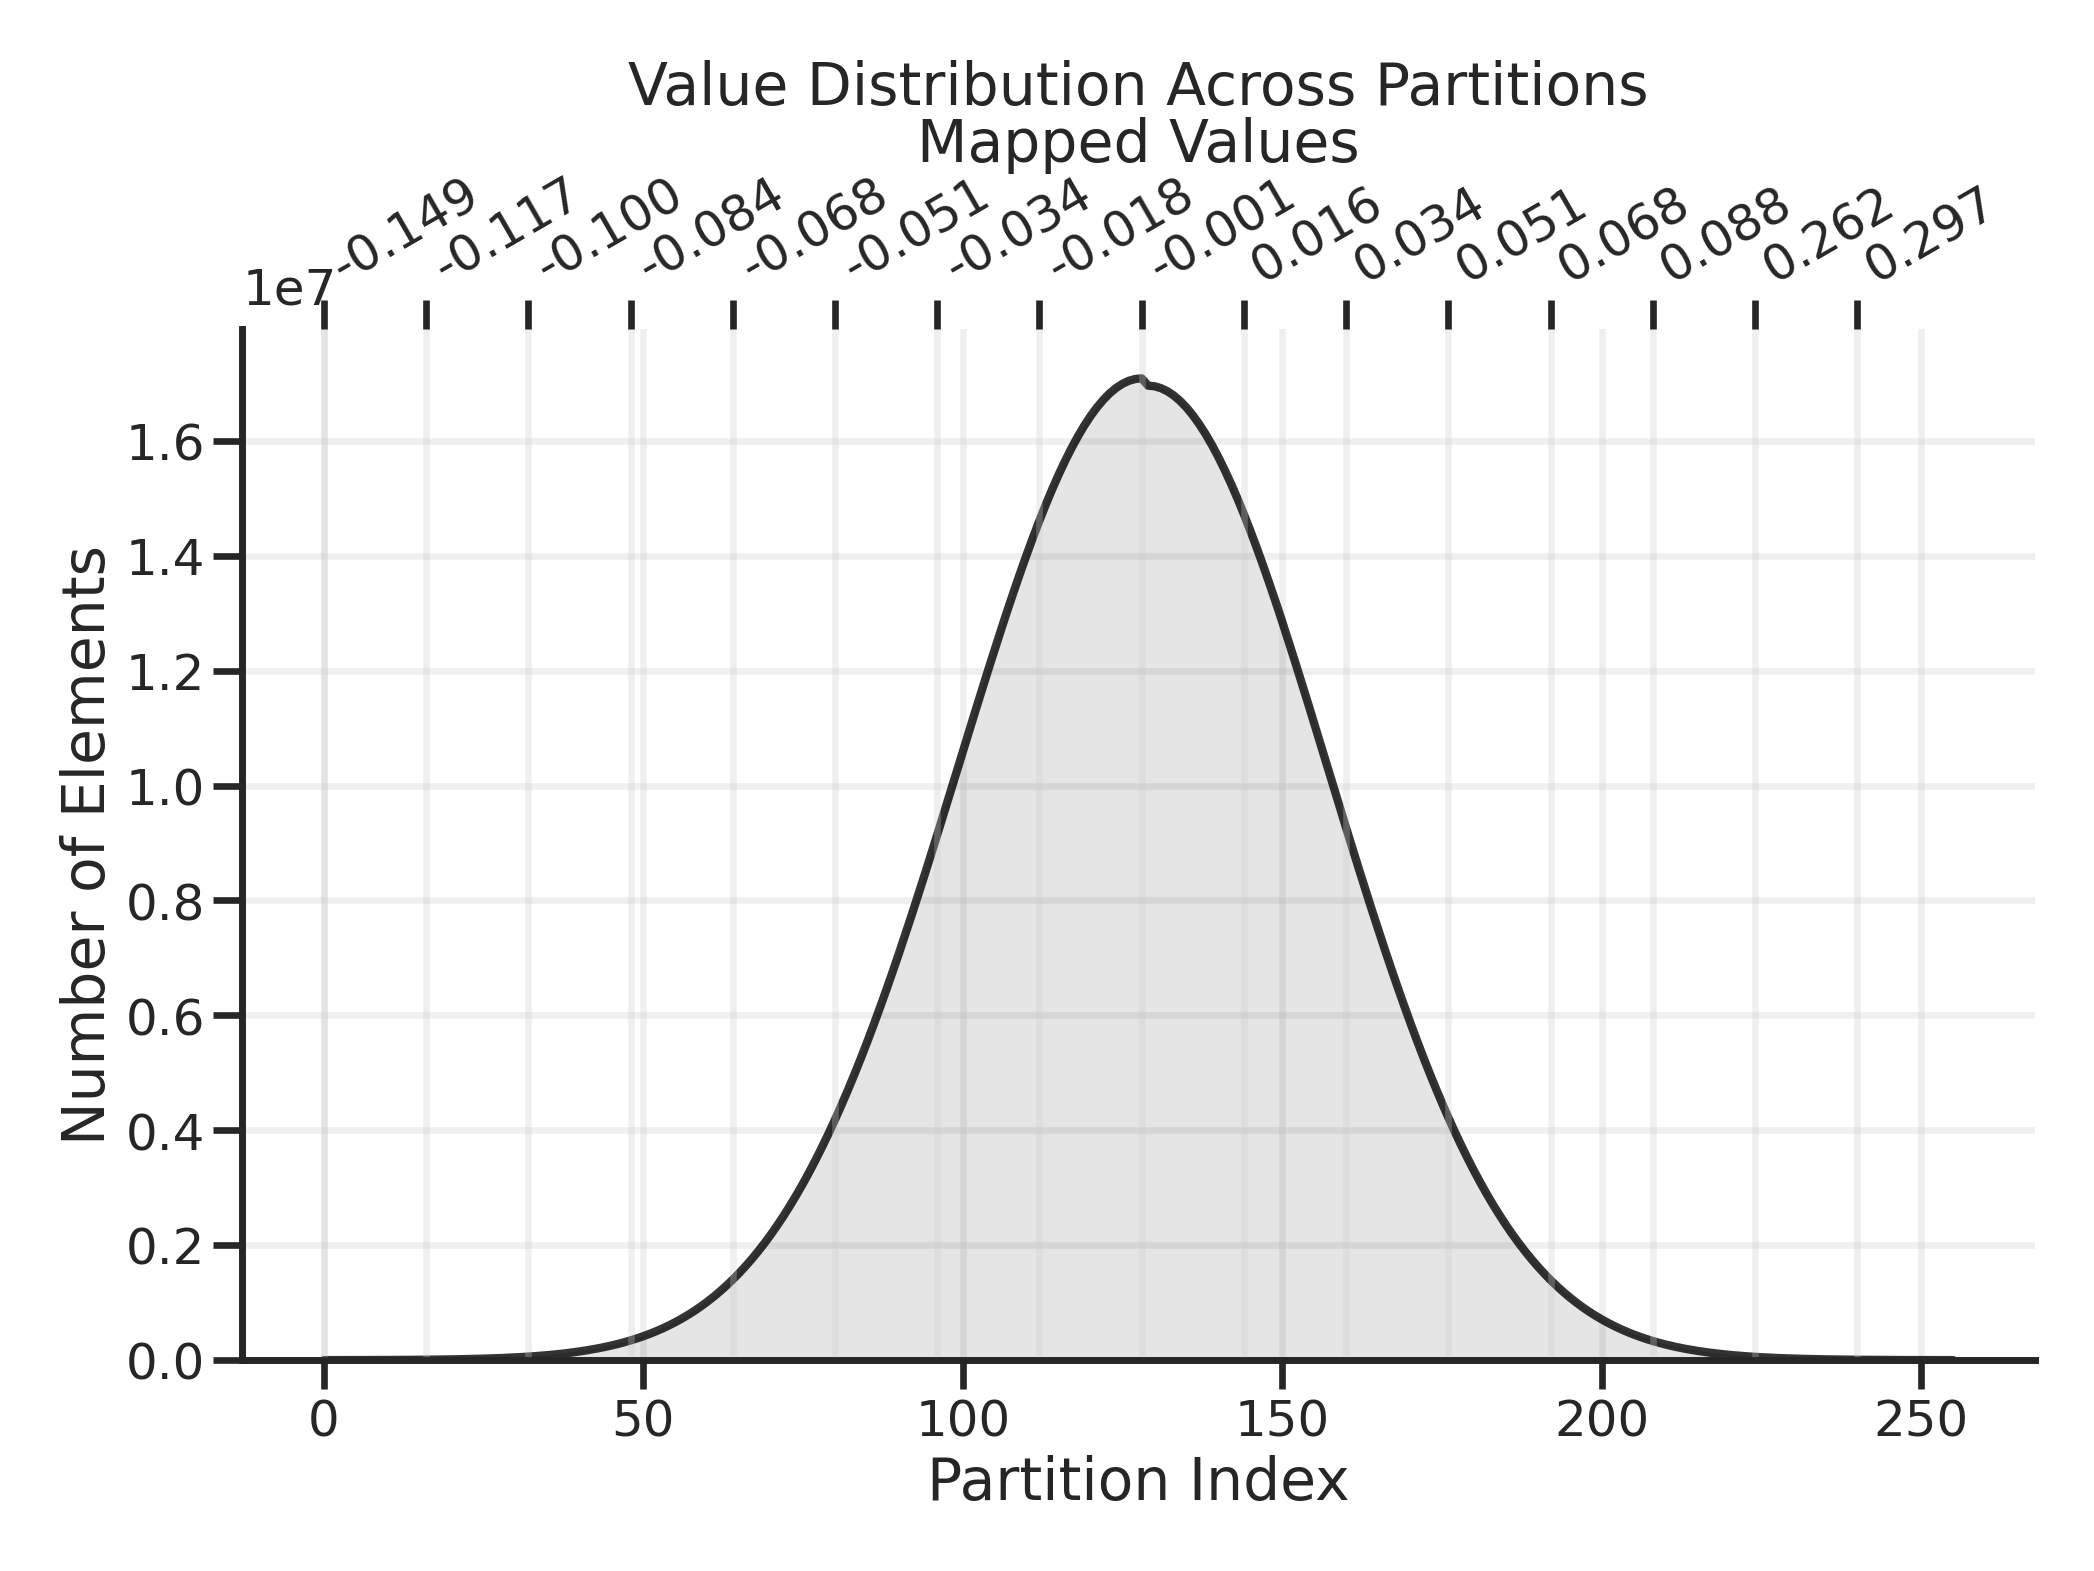
\includegraphics[width=0.49\widefigwidth]{bilder/plots/value_distribution.png}
            \vspace*{-1cm}
            \caption{\scriptsize{Value distribution of quantized test dataset}}
            \label{mfvaluedist}
        \end{minipage}
        %\hfill
        \begin{minipage}{0.49\widefigwidth}
            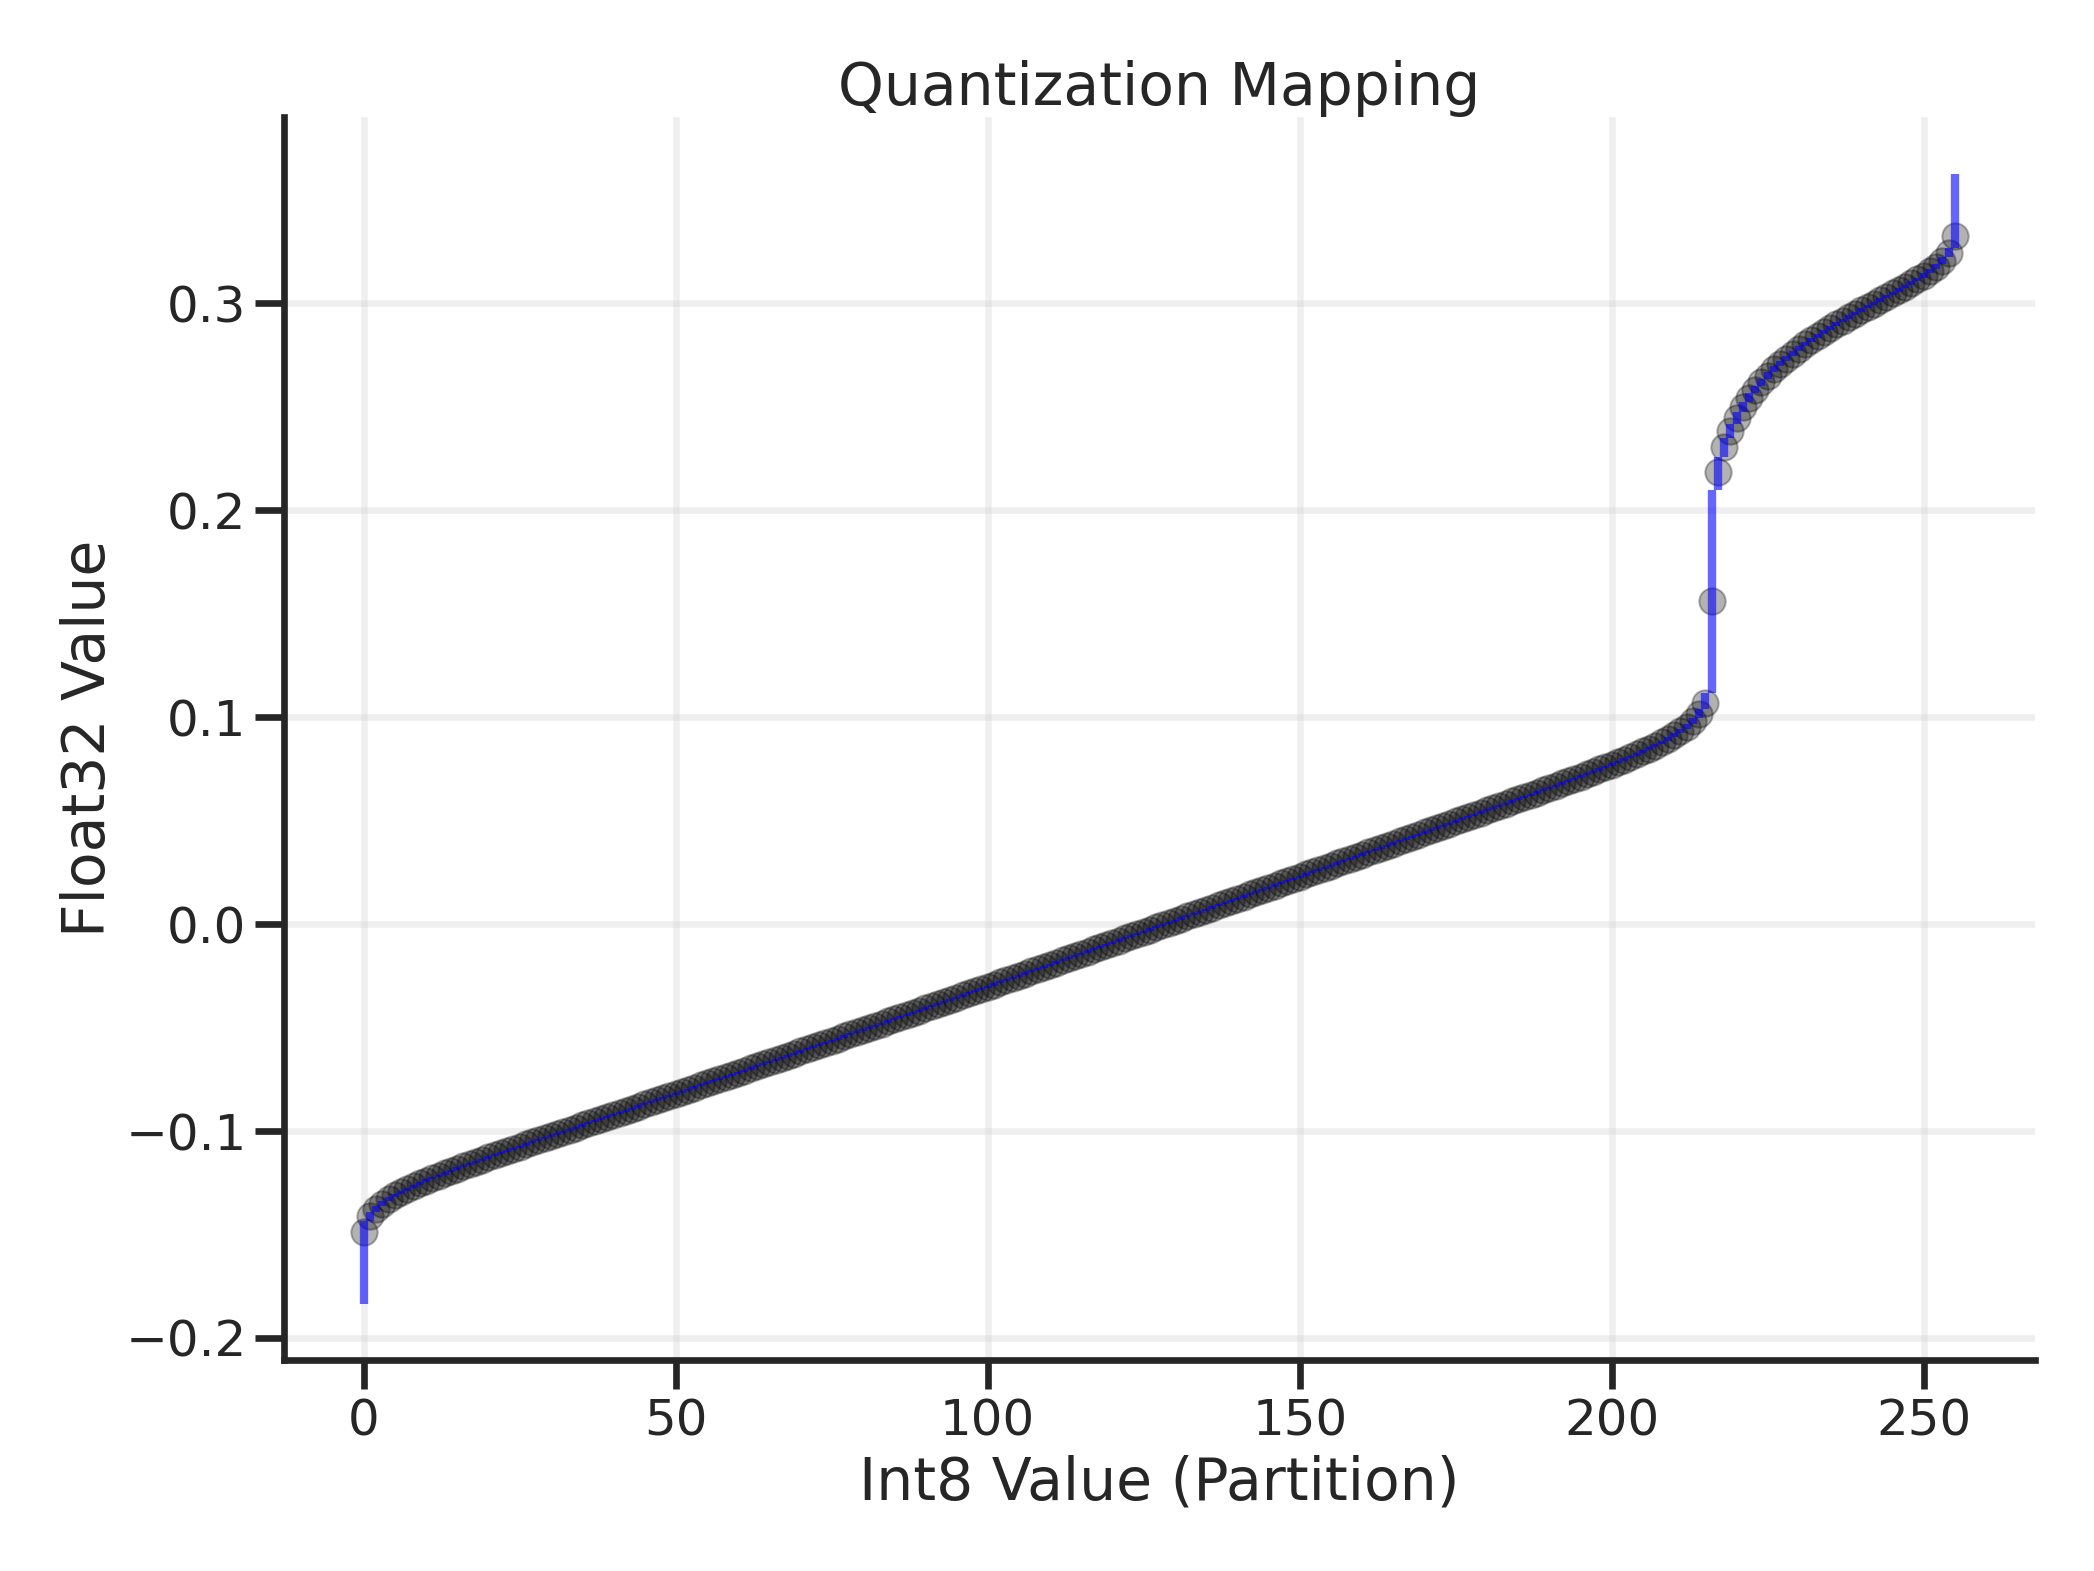
\includegraphics[width=0.49\widefigwidth]{bilder/plots/quantization_mapping.png}
            \vspace*{-1cm}
            \caption{\scriptsize{Quantization Mapping of quantized test dataset}}
            \label{mfquantmapping}
        \end{minipage}
    }
\end{figure}
The mapped float quantization uses a novel technique that combines quantization with value mapping to achieve high accuracy while reducing memory usage. Like the int8 quantization it uses 8bit integers to store the quantized values. But it doesn't just linearly map the values to the [-127, 127] range. This method analyzes the value distribution of the embedding vectors during quantization and adapts the quantized values to it.

In the first step of quantization the embedding matrix is flattened into a single array in which the float values are sorted. This gives the distribution of all values across all embeddings. For the test dataset with 1 200 000 embeddings with 1024 dimensions, this would result in 1.2 billion float values to sort.

Now the sorted values are partitioned into 256 segments using a Gaussian distribution weighting. This is implemented in the \texttt{partitionAndAverage} function:~\autoref{alg:distributionweighting}.
\begin{figure}[h]
    \begin{algorithm}{Distribution weighting}{distributionweighting}
        \begin{lstlisting}[language=C++]
double weight = std::exp(-relative_pos * relative_pos * factor);
    \end{lstlisting}
    \end{algorithm}
\end{figure}
Here \textit{relative\_pos} is the normalized position (-1 to 1). \textit{factor} controls the shape of the distribution and can be used for fine tuning. This weighting guarantees more precision in dense regions of the distribution, while also allowing outliers that are closer to -1 or 1 to keep their relatively high impact during the similarity computation.
For each partition its most important values are stored inside the \textit{PartitionInfo} struct. The average values of each partition are also stored in the \textit{mapped\_floats} array.
\begin{figure}[h]
    \begin{algorithm}{PartitionInfo and mapped\_float array}{partitioninfomappedfloatarray}
        \begin{lstlisting}[language=C++]
struct PartitionInfo {
  float start;    // First value in partition
  float end;      // Last value in partition
  float average;  // Average of all values in partition
};
alignas(32) float mapped_floats[256];
    \end{lstlisting}
    \end{algorithm}
\end{figure}
At the end of the quantization process, each float value in the original embedding is mapped to an uint8 index defined by the partitions' boundaries it fits into. The partition is efficiently searched via binary search. The cosine similarity function uses AVX2 gather instructions to efficiently load the corresponding mapped float values for the given uint8 indices as shown in~\autoref{alg:mappedfloatcosinesimilarity}.
\begin{figure}[h]
    \begin{algorithm}{Excerpt from mapped float cosine similarity}{mappedfloatcosinesimilarity}
        \begin{lstlisting}[language=C++]
__m256i indices_b = _mm256_cvtepu8_epi32(...);
__m256 values_b = _mm256_i32gather_ps(mapped_floats, indices_b, 4);
    \end{lstlisting}
    \end{algorithm}
\end{figure}
The query vector stays as is because it's kept as a float32 vector the entire time as it would make no sense to convert it to the uint8 indices and then back to float. In conclusion this method has the following advantages:
\begin{itemize}
    \item It only uses 1/4th of the memory the float32 based searchers needs.
    \item The weighted partitioning gives precise Quantization in dense areas but still can represent outliers good enough to impact the dot product.
    \item Small, 1 kB mapping table can stay in L1 cache.
    \item Gather instructions are usually to slow to make sense combining them with vector instructions. But as the mapping table stays entirely in L1 cache the latency penalty is less bad.
\end{itemize}

\section{Dimension reduction}
\label{sec:dimreduct}
Principal Component Analysis (PCA) is another approach to reduce memory usage and accelerating the search by reducing vector dimensions. The simsearch program has a function that takes the embedding matrix and a reduction factor as input. When the function is finished it will return the dimension reduced embedding matrix, the PCA-matrix and the mean vector. The latter two are required to convert search queries to the same dimension as the dimension reduced embeddings. This method uses the Eigen library to simplify the matrix and vector operations.
From now on the original vector dimension will be $d$ and $n$ is the number of embeddings. The embedding matrix will be called $M$. Logically $M$ is an $n \times d$ Matrix.

In the first step the mean vector across all embeddings is calculated and then subtracted form each vector. This centers the data around the origin and increases the PCA effectiveness.

In the next Step the $d \times d$ covariance matrix gets calculated: $Cov = \frac{(M^T \cdot M)}{n-1}$
This matrix describes the relationship between dimensions.

Now the eigenvalues and eigenvectors of the covariance matrix are calculated. The eigenvectors get sorted by descending eigenvalue magnitude. Larger eigenvalues suggest more important principal components.

Next we do the dimensionality reduction: Select top $k = d / reduction\_factor$ eigenvectors.
With these top k eigenvectors, the PCA-matrix $P$ of size $d \times k$ gets created. The original embeddings now can get dimension reduction by multiplying it with the PCA-matrix: $M_{reduced} = M \cdot P$\\
$M_{reduced}$ now has the dimensions $n \times k$.

Finally, in the last step, the vectors have to get normalized again.

\section{SIMD optimization}
\subsection{Float32 implementation with AVX2}
\label{floatimplavx2}
\begin{figure}[h]
    \begin{algorithm}{Converting float vector to AVX2}{floatvectoavx2}
        \begin{lstlisting}[language=C++]
void convertEmbeddingToAVX2(const std::vector<float> &input,
                            avx2_vector &output, size_t vector_dim) {
    for (size_t j = 0; j < vector_dim; j++) {
        size_t k = j * 8; // Each AVX2 vector holds 8 floats
        // will load 8*32bit -> input[i] .. input[i+7]
        output[j] = _mm256_loadu_ps(&input[k]);
    }
}
    \end{lstlisting}
    \end{algorithm}
\end{figure}
\begin{figure}[H]
    \begin{algorithm}{Cosine similarity for AVX2 float vectors}{cosinefloatavx2}
        \begin{lstlisting}[language=C++]
inline float _mm256_reduce_add_ps(__m256 x) {   // Sum all 8 floats in x
  __m128 high128 = _mm256_extractf128_ps(x, 1); // Get upper 4 floats
  __m128 low128 = _mm256_castps256_ps128(x);    // Get lower 4 floats
  __m128 sum = _mm_add_ps(high128, low128);     // Add hi+lo -> 4 floats
  sum = _mm_hadd_ps(sum, sum);     // Adjacent pairs -> (a+b,c+d,a+b,c+d)
  sum = _mm_hadd_ps(sum, sum);     // Final sum in lowest float
  return _mm_cvtss_f32(sum);       // Extract lowest 32-bit float
}
float cosine_similarity(const avx2_vector &a,
                        const avx2_vector &b) {
  __m256 dot_product = _mm256_setzero_ps(); // <-
  __m256 mag_a = _mm256_setzero_ps();       // <- init all 3 vars with 0
  __m256 mag_b = _mm256_setzero_ps();       // <-
  for (size_t i = 0; i < a.size(); ++i) {
    __m256 prod = _mm256_mul_ps(a[i], b[i]);        // multiply vectors
    dot_product = _mm256_add_ps(dot_product, prod); // add to running sum
    mag_a = _mm256_add_ps(mag_a, _mm256_mul_ps(a[i], a[i]));//mag_a+=a^2
    mag_b = _mm256_add_ps(mag_b, _mm256_mul_ps(b[i], b[i]));//mag_b+=b^2
  }
  float dot_product_sum = _mm256_reduce_add_ps(dot_product);
  float mag_a_sum = _mm256_reduce_add_ps(mag_a);
  float mag_b_sum = _mm256_reduce_add_ps(mag_b);
  return dot_product_sum / (sqrt(mag_a_sum) * sqrt(mag_b_sum));
}
    \end{lstlisting}
    \end{algorithm}
\end{figure}
This implementation will have the same accuracy and memory usage as the naive float implementation but it will be faster because AVX2 can multiply two vectors, consisting of 8 floats each, at once. We convert the default float vectors into AVX2 by simply loading the original vectors in 256 bit / 32 Byte steps into the AVX2 Vector as shown in \autoref{alg:floatvectoavx2}.

Computing the cosine similarity works generally like in the naive float version but with AVX2 instructions. The computation will be explained with the algorithm in \autoref{alg:cosinefloatavx2}. Line 11-13 initializes the running sums for the dot product and magnitudes. The for loop iterates over the whole vector where each element is actually an AVX2 vector with 8 float elements. Next the two vectors are multiplied. After that the product is added to the dot product. Line 17, 18 squares each vector and then adds the result to the magnitude for the corresponding vector. After the for loop the sum of all float values in the three AVX2 vectors (\textit{dot\_product}, \textit{mag\_a}, \textit{mag\_b}), also called horizontal sum, are calculated with the helper function \textit{\_mm256\_reduce\_add\_ps} in \autoref{alg:cosinefloatavx2}.

\subsection{Int8 quantization with AVX2}
\label{int8implavx2}
The conversion from float to int8 works like explained in section \autoref{int8quant}. But this time we can store 32 int8 values in one AVX2 vector. The similarity gets computet in two steps: Because the results gets stored as int16 because of the potential overflow we can actually just multiply 16 values at a time. For this we first extract the lower 128bit in line 7 and 8 and multiply in line 6. The result gets stored as 256bit value, because we extend from 16*8bit to 16*16bit during multiplication. The same happens with the higher 128 bits in line 9-11. In the last step we add the \textit{mul\_lo} and \textit{mul\_hi} products to their corresponding running sum \textit{sum\_lo} and \textit{sum\_hi}. After the loop we build the horizontal sum of the two running sum vectors.

\begin{figure}[h]
    \begin{algorithm}{Cosine similarity for int8 with AVX}{cosineint8avx2}
        \begin{lstlisting}[language=C++]
uint cosine_similarity(const avx2i_vector &a,
                       const avx2i_vector &b) {
  __m256i sum_lo = _mm256_setzero_si256();// Accum. for lower 128 bits
  __m256i sum_hi = _mm256_setzero_si256();// Accum. for upper 128 bits
  for (size_t i = 0; i < a.size(); ++i) { // 32 elements per iteration
    __m256i mul_lo = _mm256_mullo_epi16(  // extr and mult lower 128 bits
        _mm256_cvtepi8_epi16(_mm256_extracti128_si256(a[i], 0)),
        _mm256_cvtepi8_epi16(_mm256_extracti128_si256(b[i], 0)));
    __m256i mul_hi = _mm256_mullo_epi16(  // extr and mult upper 128 bits
        _mm256_cvtepi8_epi16(_mm256_extracti128_si256(a[i], 1)),
        _mm256_cvtepi8_epi16(_mm256_extracti128_si256(b[i], 1)));
    sum_lo = _mm256_add_epi32(sum_lo, // Accum. into 32bit to prev overfl
               _mm256_madd_epi16(mul_lo, _mm256_set1_epi16(1)));
    sum_hi = _mm256_add_epi32(sum_hi, // Accum. into 32bit to prev overfl
               _mm256_madd_epi16(mul_hi, _mm256_set1_epi16(1)));
  } // horizontal sum gets built and returned here
}
    \end{lstlisting}
    \end{algorithm}
\end{figure}

\subsection{Binary quantization with AVX2}
\label{binaryquantavx2}
\begin{figure}[h]
    \begin{algorithm}{Cosine similarity for binary with AVX}{cosinebinaryavx2}
        \begin{lstlisting}[language=C++]
int EmbeddingSearchBinaryAVX2::cosine_similarity(const avx2i_vector &a,
                                                 const avx2i_vector &b) {
  int dot_product = 0;
  __m256i all_ones = _mm256_set1_epi32(-1); // set every bit to 1
  for (size_t i = 0; i < a.size(); ++i) {
    __m256i result = _mm256_xor_si256(a[i], b[i]); // XOR
    result = _mm256_xor_si256(result, all_ones);   // NOT
    uint64_t *result_ptr = reinterpret_cast<uint64_t *>(&result);
    dot_product += __builtin_popcountll(result_ptr[0]); // sum all 64 bit
    dot_product += __builtin_popcountll(result_ptr[1]); // popcounts for
    dot_product += __builtin_popcountll(result_ptr[2]); // 256 bit result
    dot_product += __builtin_popcountll(result_ptr[3]);
  }
  return dot_product;
}
    \end{lstlisting}
    \end{algorithm}
\end{figure}
Just like in \autoref{binaryquant} we just store the sign of the float embeddings. This time we can store 256 binary values in one AVX2 vector. Cosine similarity is computed by using XOR on both 256 bit vectors and then using XOR with a vector full of ones on the result. This flips every bit of the result. After that we have the XNOR result. We have to use \textit{popcountll} four times because each can only build the popcount of 64 bits. See \autoref{alg:cosinebinaryavx2}.

\subsection{Optimized float32 implementation with AVX2}
\label{floatoavx2}
Like explained in \autoref{memorymanagement} the optimized implementation uses manually managed memory to store the embeddings. The embeddings are set using memcpy.
% The cosine similarity works different (see \autoref{alg:cosinefloatoavx2}): Here the similarity function only gets a pointer to the vectors.
% Furthermore, the function expects both vectors to be normalized already. This way it doesn't have to calculate that magnitudes of the vectors, which also saves some computation time.
% In addition to this loop unrolling is used. One loop iteration works through 8 vectors instead of one. Although modern CPUs and compilers can unroll loops on their own it is implemented it manually here. The unroll factor is 8. That means 16 AVX vectors are loaded per iteration, which makes perfect use of the 16 256-bit AVX registers \cite{intel64manual}.
% Beyond that line 20-23 use a prefetching instruction to preload vectors into cache that will be accessed within a few loop iterations. This can also help, especially if it's fine-tuned for the used hardware \cite{prefetching}.
% Finally, this implementation also uses fused multiply-add, which has the benefit of being faster, more accurate due to less rounding and being more predictable \cite{fma}.
% At last the horizontal sum is calculated the same way the unoptimized AVX2 version does \autoref{floatimplavx2}.
A key optimization of this implementation is the use of strided memory access which increases memory bandwidth in combination with a more efficient vector loading strategy. This seems to be contrary to common knowledge, because sequential memory access should always be preferred it was also tested in isolation here \autoref{section:stridedmembwtest}.
The stride distance automatically gets adapted to the vector size as the stride length being a multiple of 4 KB seems to give the highest memory bandwidth. A reason for this could be the systems' page size, which is 4 KB. So accessing multiple pages at once could increase the bandwidth. Another reason could be memory interleaving.
This implementation also uses fused multiply-add (FMA), which has the benefit of being faster and more accurate due to less rounding and being more predictable.~\cite{fma}

The optimized vector loading leverages the fact, that the query vector stays the same across all comparisons. The result of this is just 7 loads (1 for query, 6 for embeddings) for 6 FMA instructions instead of 12 loads (6 for query, 6 for embeddings) for the same amount of FMA instructions. The loaded part of the query vector can also stay in one register while being multiplied with the 6 embeddings. This can be seen in \autoref{alg:cosinefloatoavx2}
Additionally, the regular pattern of 7 loads followed by 6 FMA instructions allows the CPU to better predict and optimize instruction execution.
The function expects both vectors to be normalized already. This way it doesn't have to calculate that magnitudes of the vectors, which also saves some computation time.

\begin{figure}[h]
    \begin{algorithm}{Cosine similarity for optimized AVX2 float vectors}{cosinefloatoavx2}
        \begin{lstlisting}[language=C++]
inline void cosine_similarity_optimized(
    const float *vec_a, float *sim, float *emb_ptr[]) {
  __m256 sum[NUM_STRIDES] = {_mm256_setzero_ps()}; // sum for all embeds
  __m256 a;              // 1 query
  __m256 b[NUM_STRIDES]; // load NUM_STRIDES(=6) embeddings at once
  for (int i = 0; i < padded_dim; i += 8) {
    a = _mm256_load_ps(vec_a + i);        // load query vec
    b[0] = _mm256_load_ps(emb_ptr[0] + i);//emb_ptr[0] pnts to curr. vec
    // do the same for indices 2,3,4 ...
    b[5] = _mm256_load_ps(emb_ptr[5] + i);//pnts to 5*strd_dst vec ahead
    sum[0] = _mm256_fmadd_ps(a, b[0], sum[0]); // FMA: sum += a * b[0]
    // do the same for indices 2,3,4 ...
    sum[5] = _mm256_fmadd_ps(a, b[5], sum[5]); // FMA: sum += a * b[5]
  } // compute horizontal sum for each sum and write to sim array ...
}
    \end{lstlisting}
    \end{algorithm}
\end{figure}
In \autoref{alg:embsearchloatoavx2} can be seen how the \textit{embedding\_search} function prepares the array of pointers to the vectors \textit{STRIDE\_DIST} apart (for loop line 6-8).
The loop starting at line 1 increments the index by \textit{NUM\_STRIDES * STRIDE\_DIST}, because that's the distance the inner loop (line 3-11) covers.
\begin{figure}[h]
    \begin{algorithm}{Excerpt from embedding\_search function of optimized AVX2 float class}{embsearchloatoavx2}
        \begin{lstlisting}[language=C++]
for (size_t i = 0; (i + (NUM_STRIDES * STRIDE_DIST) - 1) < num_vectors;
       i += (NUM_STRIDES * STRIDE_DIST)) { // inc by total dist covered
    for (size_t j = i; j < (i + STRIDE_DIST); j++) { // by inner loop
      float sim[NUM_STRIDES] = {}; // cosine fn writes result into this
      float *emb_ptr[NUM_STRIDES]; // arr of ptrs to vectors STRIDE_DIST
      for (int k = 0; k < NUM_STRIDES; k++) { // apart
        emb_ptr[k] = get_embedding_ptr(j + k * STRIDE_DIST);
      }
      cosine_similarity_optimized(query_aligned.data(), sim, emb_ptr);
      // store results...
    }
  }
    \end{lstlisting}
    \end{algorithm}
\end{figure}

\subsection{Optimized int8 implementation with AVX2}
\label{sec:optint8avx2}
The cosine function of this is mostly similar to the one already presented in \autoref{int8implavx2}. It uses the memory in the same way as the optimized float32 implementation in \autoref{floatoavx2}.
\subsection{Optimized binary implementation with AVX2}
\label{sec:optbinaryavx2}
\begin{figure}[h]
    \begin{algorithm}{Cosine similarity for optimized AVX2 binary vectors}{cosinebinaryoavx2}
        \begin{lstlisting}[language=C++]
int32_t cosine_similarity_optimized(const __m256i *vec_a,
                                    const __m256i *vec_b) const {
  // prefetch 2 cache lines for 4 vectors 10 loops ahead
  _mm_prefetch(vec_a + 4 * 10, _MM_HINT_T0);
  _mm_prefetch(vec_a + 4 * 10 + 2, _MM_HINT_T0);
  __m256i all_ones = _mm256_set1_epi32(-1);
  __m256i xor_result[4];
  xor_result[0] = _mm256_xor_si256(vec_a[0], vec_b[0]);      // XOR
  xor_result[0] = _mm256_xor_si256(xor_result[0], all_ones); // NOT
  xor_result[1] = _mm256_xor_si256(vec_a[1], vec_b[1]);      // XOR
  xor_result[1] = _mm256_xor_si256(xor_result[1], all_ones); // NOT
  // do the same for indices 2 and 3
  // popcnt lookup is faster than harley seal and builtin
  return counter.popcnt_AVX2_lookup( // optimized version using AVX2
      reinterpret_cast<const uint8_t *>(xor_result),
      4 * sizeof(__m256i));
}
    \end{lstlisting}
    \end{algorithm}
\end{figure}
\noindent The embeddings are set similarly to method described in \autoref{binaryquant} and \autoref{binaryquantavx2}. Like the optimized float implementation in \autoref{floatoavx2}. This cosine implementation also uses loop unrolling and manual prefetching. The XNOR based binary multiplication matches the previous one in \autoref{binaryquantavx2}. But a big improvement is the usage of 256-bit popcount algorithm implemented with AVX2 instructions, which was developed by \citeauthor{Mu_a_2017}.~\cite{Mu_a_2017} Cosine similarity algorithm can be seen here \autoref{alg:cosinebinaryoavx2}.

\section{Two-step search with rescoring}
\label{sec:twostep}
The two-step approach uses a fast but lower accuracy search first to filter for candidates. Then a full accuracy search is done on these candidates. The top results from the second search are the final result. The goal of this method is to combine the speed of the lower accuracy search with the high accuracy of full precision search. The amount of documents the first search retrieves can be tuned with the rescoring factor. The amount of documents retrieved by the first searcher is defined by $rescoring\_factor * k$. In the second step the top $k$ documents will be retrieved. There are two two-step searchers that will be tested: The first is implemented using the optimized versions of the binary and float32 searchers displayed in \autoref{alg:twostep}. The second one uses the optimized binary searcher and the mapped float searcher for rescoring.

\begin{figure}[h]
    \begin{algorithm}{Two-step search with binary searcher and full precision searcher}{twostep}
        \begin{lstlisting}[language=C++]
// Binary search for initial filtering
auto binary_results = binary_avx2_searcher->similarity_search(
    queryBinaryAvx2,     // Binary query vector
    k * rescoring_factor // Get more candidates for rescoring
);
// Full precision rescoring
auto avx2_results = avx2_searcher->similarity_search(
    query,              // Original float query
    k,                  // Final number of results
    binary_results      // Pre-filtered candidates
);
        \end{lstlisting}
    \end{algorithm}
\end{figure}
% Execution Time Comparison
\chapter{Experimental evaluation}
\label{chapter:exp_eval}
\section{Methodology}
\subsection{Dataset}
The dataset which will be used for benchmarking the optimization methods described in the previous chapters is the Wikipedia article dataset from Wikimedia available on hugging face\footnote{\url{https://huggingface.co/datasets/wikimedia/wikipedia}}.
This set contains over 6 million English articles from Wikipedia.
Instead of encoding all articles, which would result in almost 23 GB in vector embeddings, 1.2 million randomly selected articles were encoded resulting in 4.6 GB of embeddings for 1024 dimensions.
The data was converted by two different embedding models: The first one is the \texttt{\seqsplit{mixedbread-ai/mxbai-embed-large-v1}} model which is a very good performing model on the \textit{Massive Text Embedding Benchmark} (available here\footnote{\url{https://huggingface.co/spaces/mteb/leaderboard}}) paper.~\cite{muennighoff2023mtebmassivetextembedding} This is a vector angle optimized model \cite{li2024angleoptimizedtextembeddings} which should give binary quantization an advantage compared to traditional models. Additionally, this model embeds to 1024 vector dimensions and has 335M parameters. To have a comparison the dataset of 1.2 million articles will be encoded with the \texttt{\seqsplit{sentence-transformers/all-mpnet-base-v2}} model available here\footnote{\url{https://huggingface.co/sentence-transformers/all-mpnet-base-v2}}. This model maps the encoded text to 768 dimensions and has 109M parameters. It scores a bit worse on the \textit{Massive Text Embedding Benchmark} but is still a solid model (rank 117 of 476 for the sentence-transformer model compared to 35 of 476 for the mixedbread-ai model as of 2024-11-29).

Unless mentioned or annotated otherwise the results and figures presented in this chapter use the \texttt{\seqsplit{mixedbread-ai/mxbai-embed-large-v1}} model with retrieval for top 100 (k=100) documents.

To benchmark the different search methods a list containing 303 queries will be used. It contains long and short-, specific and unspecific-, pointless queries, etc.

\begin{table}[h]
    \centering
    \begin{tabular}{lcr}
        \toprule
        Method Name                                                          & Short Name             & Section                     \\
        \midrule
        naive float                                                          & float                  & \autoref{naivefloat}        \\
        Optimized Bianry with AVX2                                           & binary                 & \autoref{sec:optbinaryavx2} \\
        Optimized Int8 with AVX2                                             & int8                   & \autoref{sec:optint8avx2}   \\
        Float16                                                              & float16                & \autoref{sec:float16}       \\
        Mapped Float                                                         & mf                     & \autoref{sec:mappedfloat}   \\
        PCAX (X indicates reduction factor)                                  & pcaX                   & \autoref{sec:dimreduct}     \\
        \footnotesize Two-Step Binary + Float (X indicates rescoring factor) & twostep\_rfX | ts\_rfX & \autoref{sec:twostep}       \\
        \footnotesize Two-Step Binary + Mapped Float (X ind. resc. factor)   & ts\_mf\_rfX            & \autoref{sec:twostep}       \\
        \bottomrule
    \end{tabular}
    \caption{Short names used in plots}
    \label{shortnames}
\end{table}

\subsection{Evaluation metrics}
To evaluate the benchmark results the Jaccard index and NDCG will be used to compare the performance to the naive float implementation as a baseline. Additionally, the time taken for each search will be measured. This includes initialization of the results array, calculating the similarity for every embedding, sorting for top k results and returning the result. At last the theoretical memory usage will be calculated, see \autoref{memorycalc}.

\begin{table}[h]
    \centering
    \begin{tabular}{lcr}
        \toprule
        Method    & Formula for embedding size in bytes                                       \\
        \midrule
        general   & $sizeof(datatype) * vector\_dim * num\_embeddings$                        \\
        rescoring & $general(binary) + general(rescoring\_method) $                           \\
        PCA       & $general(datatype) + vector\_dim * (reduced\_dim + 1) * sizeof(datatype)$ \\
        \bottomrule
    \end{tabular}
    \caption{Calculation of memory used for different methods}
    \label{memorycalc}
\end{table}

\begin{table}[h]
    \centering
    \begin{tabular}{lccr}
        \toprule
        Method                         & Memory usage                                  & Mem. usage test Dataset \\
        \midrule
        float (including avx2 version) & $base$                                        & 4.58 GB                 \\
        binary                         & $\frac{base}{32}$                             & 0.14 GB                 \\
        int8                           & $\frac{base}{4}$                              & 1.14 GB                 \\
        float16                        & $\frac{base}{2}$                              & 2.29 GB                 \\
        mapped float                   & $\frac{base}{4} + 1kB$ for mapping table      & 1.14 GB                 \\
        PCA by factor $x$ (float)      & $\frac{base}{x} + d * (\frac{d}{x} + 1) * 4B$ & $\sim\frac{4.58 GB}{x}$ \\
        two-step binary+float          & $base + \frac{base}{32}$                      & 4.72 GB                 \\
        two-step binary+mapped float   & $base + \frac{base}{4} + 1kB$                 & 1.29 GB                 \\
        \bottomrule
    \end{tabular}
    \caption{Memory usage as ratio to baseline\\\footnotesize{d=vector dimension}}
\end{table}

\subsection{Testing environment}
All benchmarks were recorded on Linux using kernel version 6.11. Specifically version \texttt{\seqsplit{6.11.10-300.fc41.x86\_64}} shipped by fedora.
The test system has an AMD 5950X CPU (16C/32T) with disabled turbo boost to get a consistent frequency of 3.4GHz.
Furthermore, 128 GB of dual-channel/quad-rank DDR4 SDRAM running at 3600MTs/1800MHz with CL18 was used.

\section{Expected Outcome}
No implementation can have the same accuracy as the float32 variants as every type of quantization and dimension has some kind of information loss.
The binary method should be by far the fastest as it has very little data to work through, resulting from its heavy quantization, and efficient multiplication method. In return the accuracy should be fairly low. The float16 should be fairly good as using it for machine learning is already quiet common.
The int8 implementation should be around 2 to 4 times faster than the optimized float32 version, as it does 16 multiplications at once compared to 8 and integer math can be faster depending on architecture. The mapped float implementation should have good accuracy, better than int8 but worse than float16 as its accuracy is much higher. The performance can be good if it's not bottlenecked by the random access latency on the mapping table.
The search speed on the PCA variants should scale linear as the dimension decreases. PCA2 should decrease the search speed to about half (plus a little overhead) compared to the AVX2 float variant, as they both use the same implementation. With the only difference that PCA has the applied dimension reduction. The accuracy for the PCA searchers is hard to predict, but if there are redundant dimensions they should perform quiet good.

\section{Results and Analysis}
\subsection{Search Time comparison}
\begin{figure}[h]
    \makebox[\textwidth][c]{%
        \begin{minipage}{0.49\widefigwidth}
            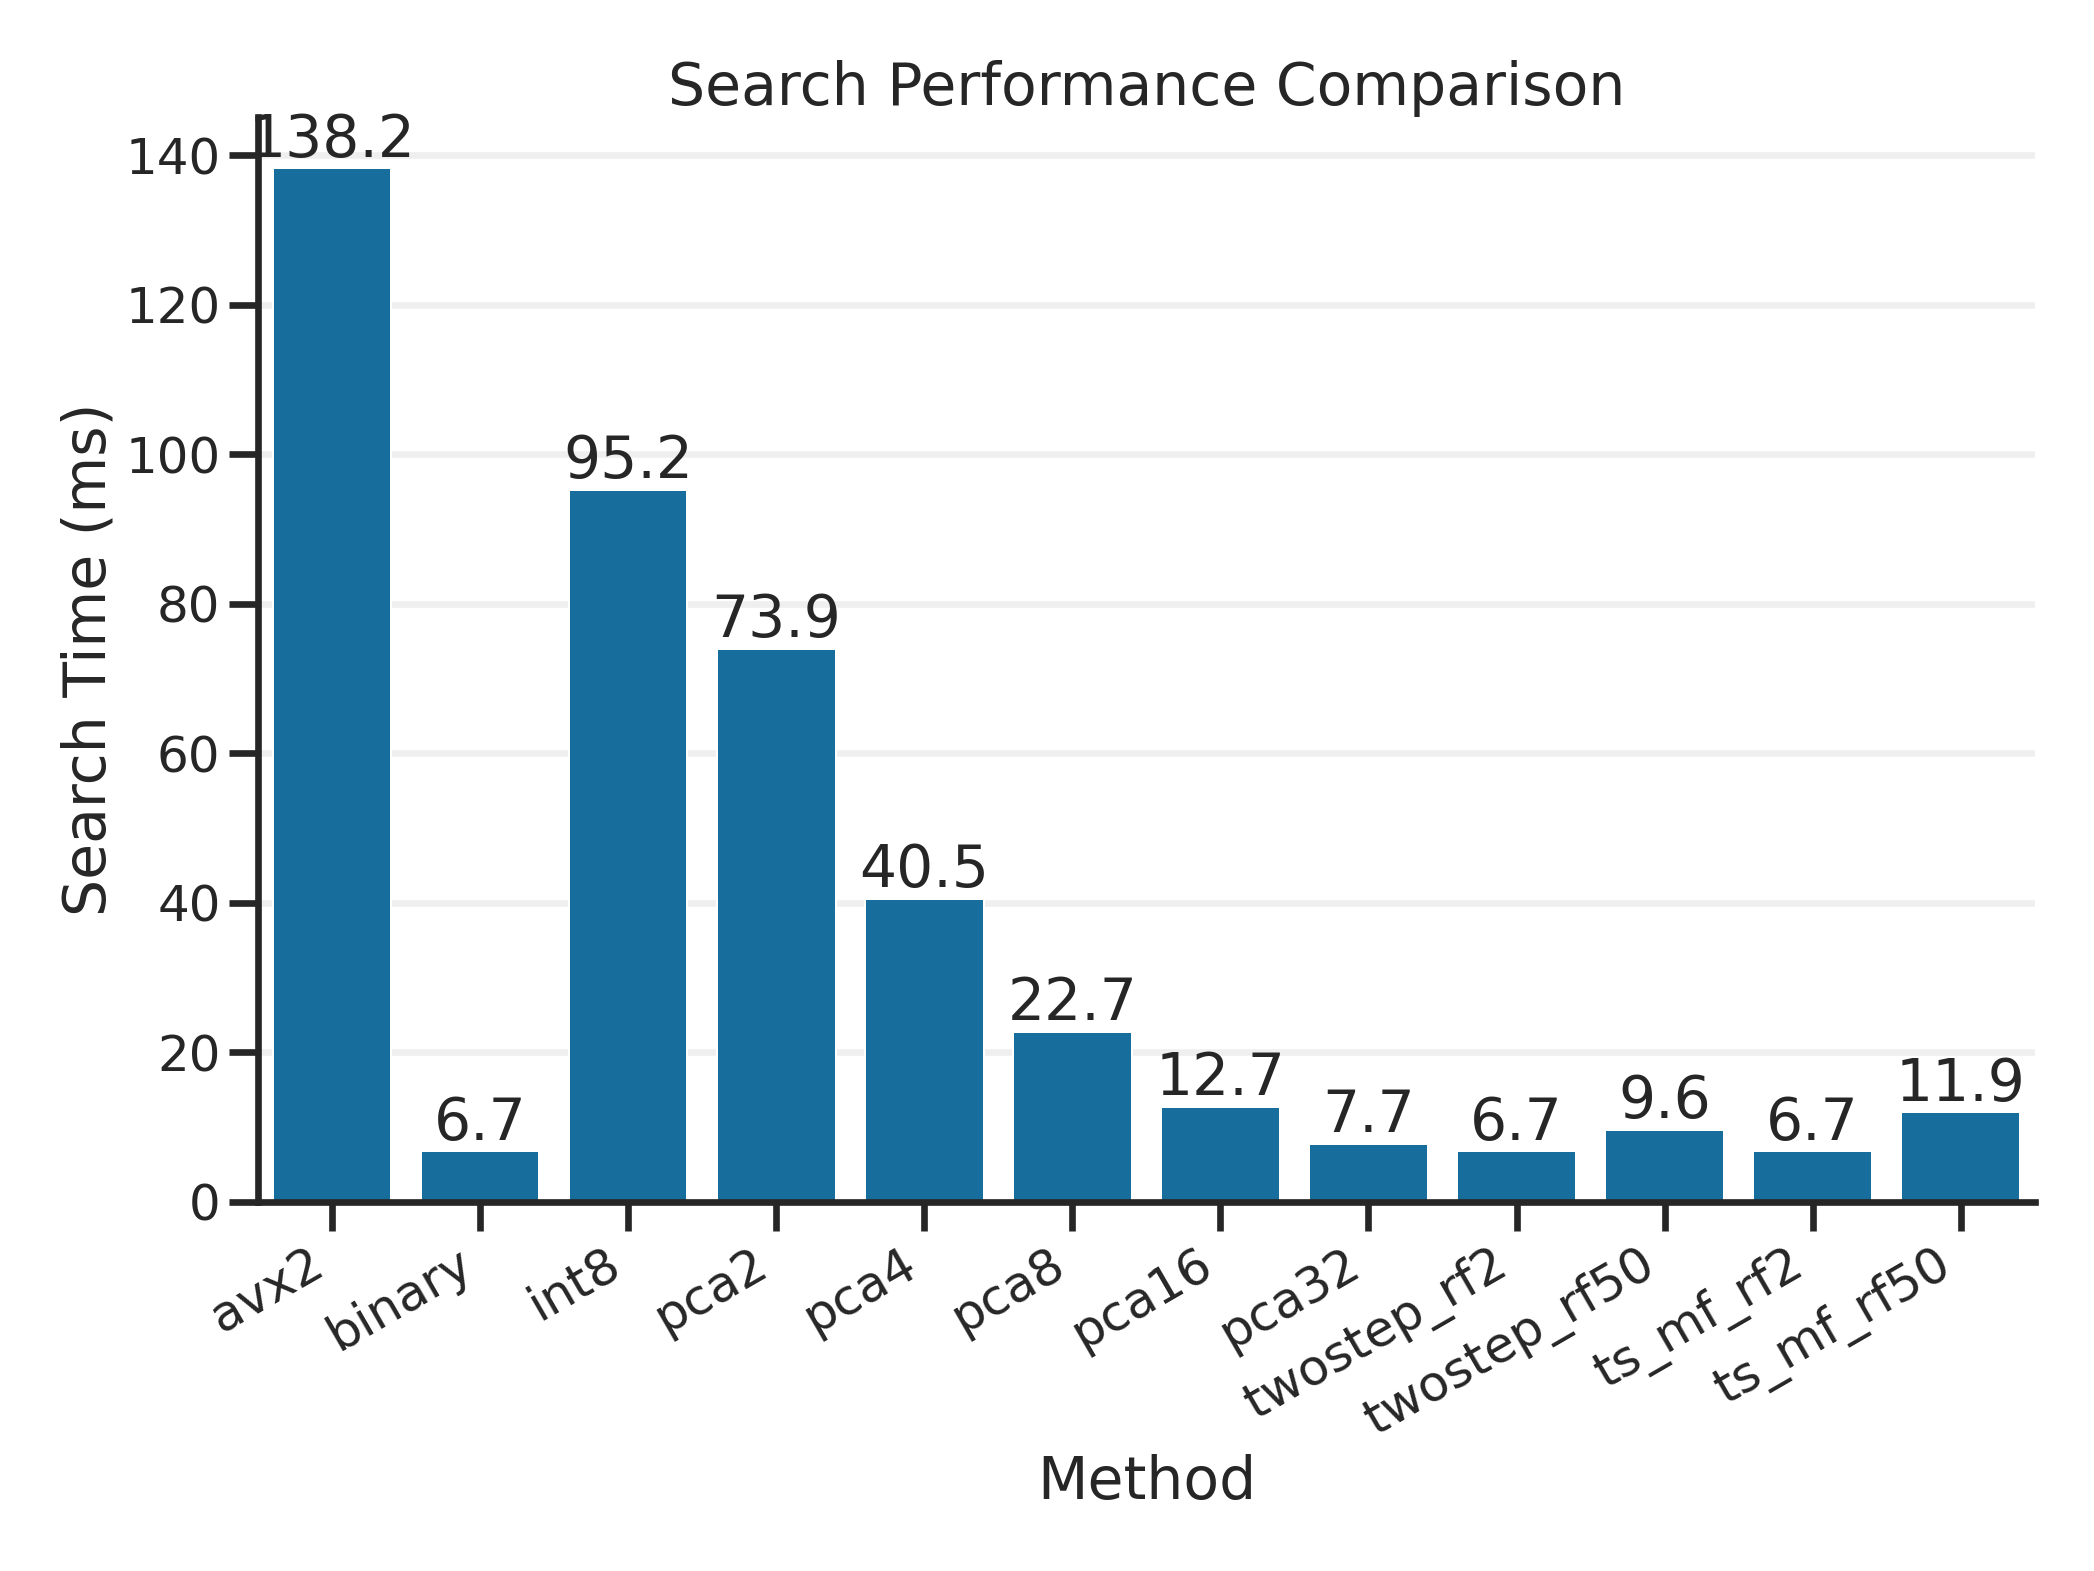
\includegraphics[width=0.49\widefigwidth]{bilder/plots/performance_comparison_dim1024_k100_q.png}
            \vspace{-1cm}
            \caption{Search Speed vec\_dim=1024}
            \label{searchspeed}
            \centering
            \small{float (1100 ms) and mapped float (540 ms) ommited}
        \end{minipage}
        %\hfill
        \begin{minipage}{0.49\widefigwidth}
            \vspace{-0.375cm}
            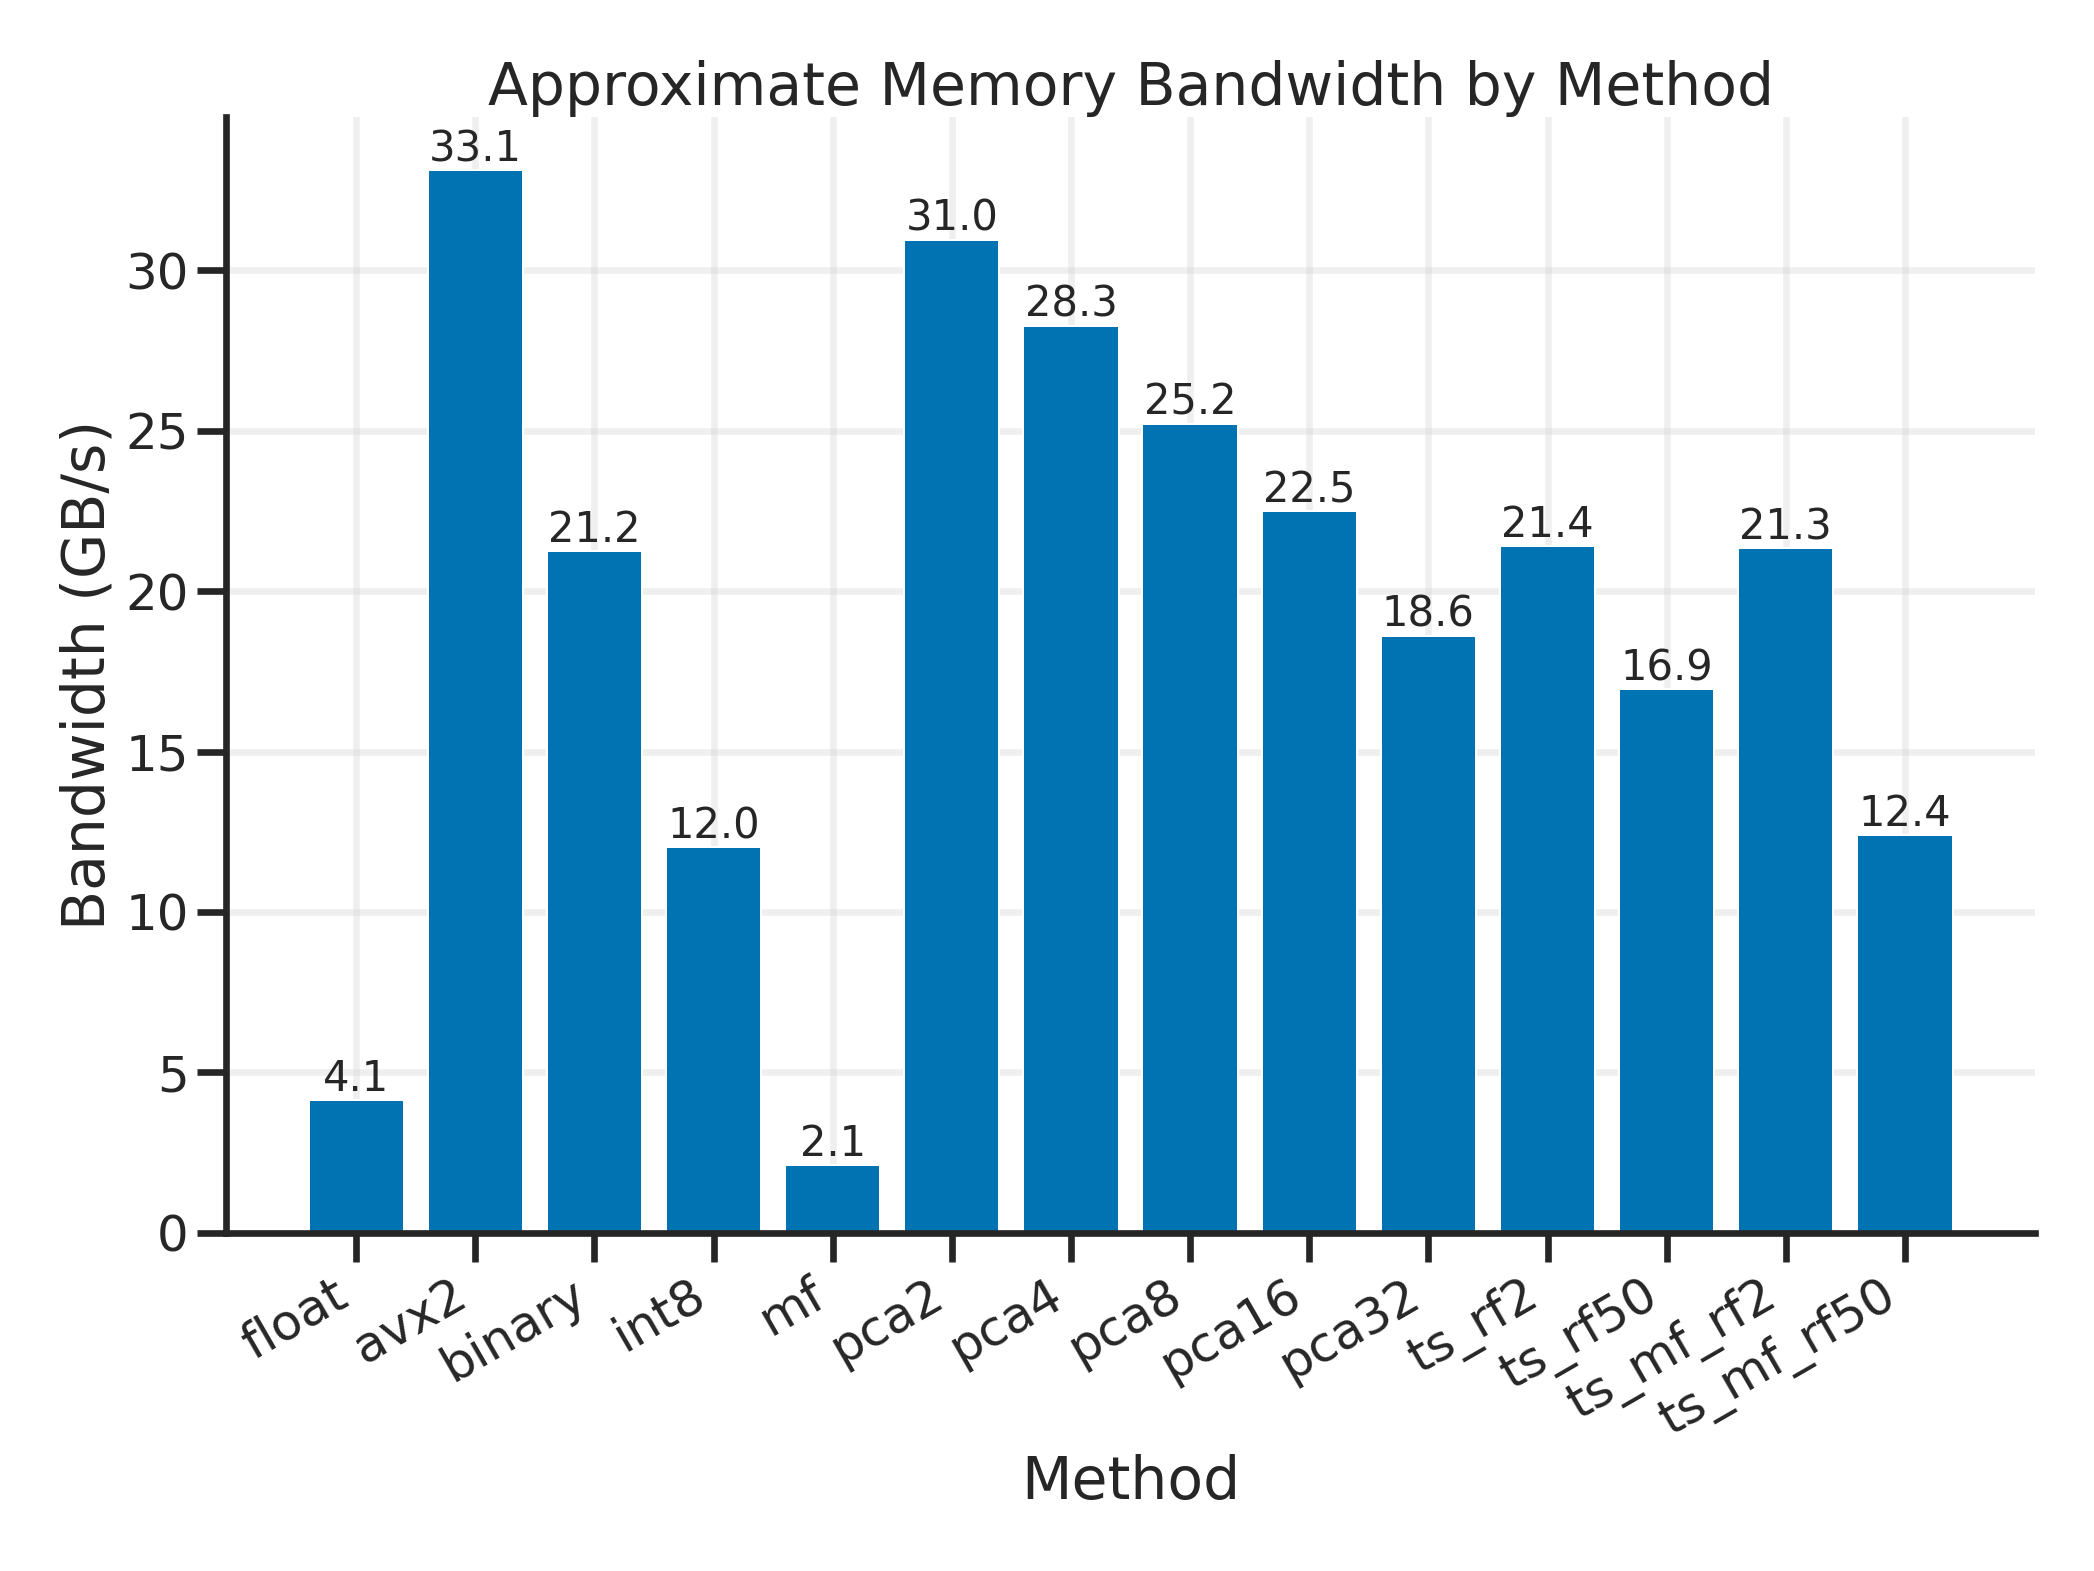
\includegraphics[width=0.49\widefigwidth]{bilder/plots/memory_bandwidth_benchmark_dim1024_k100_q.png}
            \vspace{-1cm}
            \caption{Memory bandwidth vec\_dim=1024}
            \label{memorybandwidth}
        \end{minipage}
    }
\end{figure}
Starting with \autoref{searchspeed}: As expected the AVX2 optimized version is much faster than the naive implementation. The fact it's 8 times faster, taking only 138.2 ms compared to 1100 ms for float, shows that this implementation makes efficient use of the AVX2 instructions.

The binary implementation, which also uses AVX2, is over 23 times faster than the AVX2 float equivalent and over 160 times faster than the baseline float implementation. Which makes sense, because it only has to iterate through $1/32$th of the data and uses efficient nor, xor and popcount instructions.

With 95 ms The int8 implementation is slower than expected. But that is likely due to the fact that AVX2 can't multiply 32 int8 values at once. It has to extract the lower/higher 128 bits, extend them to 16bit and then do 2 multiplications for the high and low values. After that it has to build the horizontal sum and add the high and low multiplication result to the running sum. This is a significant amount of instructions compared to the AVX2 float implementation where 32 floats are multiplied and added to the running sum by just 4 FMA instructions.

The PCA variants perform quiet well. The dimension reduction to half almost doubles the search speed compared to the float AVX2 implementation, which makes sense, given the fact that the vectors only have half the dimensions. The other PCA factors almost scale linearly as well. Which suggests, that the overhead from the functions involved calculating the similarities is very low. PCA4 is more than 2 times faster than int8 which has to go through the same amount of data. This shows that AVX2 doesn't really perform well at multiplying int8 values.

The two-step method based on the binary and float AVX2 implementation is very close to the pure binary search time. Even for high numbers of retrieved documents and rescoring factors, the amount of embeddings the second step method has to search is very small, e.g. 5000 for k=100 and rescoring factor of 50 (like in \autoref{searchspeed}), compared to the total number of embeddings.

With 540ms the mapped float searcher has the second-worst search time after the naive float. The reason for this being, that the CPU prefetcher can only predict the int8 values that will be loaded next. But after this gather instructions are used to load the corresponding float values from the mapping table. Even though it's very small (1 KB) and likely stays in L1 cache the entire time, even the very low L1 cache latency of around 1ns adds up: Taking the benchmarked dataset with 1.2M embeddings with 1024 dimensions it would take $10^{-9} s * 1024 * 1.2 * 10^{6} / 8 = 153.6 ms$ just to load the float values for the embeddings. And this makes the assumption, that loading 8 float values at once takes 1ns. In conclusion, this methods' reliance on random memory access slows the search significantly. This is also seen in the low memory bandwidth in \autoref{memorybandwidth}.

Finally, the two-step method using binary and the mapped float performs similar to binary just like the two-step method that uses full accuracy search in the second step. Only as the rescoring factor increases it takes slightly longer than its competitor. That happens, because the mapped float searcher is much slower than the avx2 searcher and as the rescoring factor increases the speed of the second-step searcher becomes more relevant. Nonetheless, this search method performs really well, as long the rescoring factors are reasonable.

\subsection{Accuracy Analysis}
The AVX2 implementation has perfect accuracy as seen in \autoref{accuracyheatmapone}. But one can spot one outlier for the Jaccard index and NDCG score in \autoref{boxjaccardsearchersone} and \autoref{boxndcgsearchersone} respectively. But that is likely due to the fact that the AVX2 implementation can actually be more accurate with the fused multiply add instruction, which eliminates one rounding step.

\begin{figure}[h]
    \makebox[\textwidth][c]{%
        \begin{minipage}{0.49\widefigwidth}
            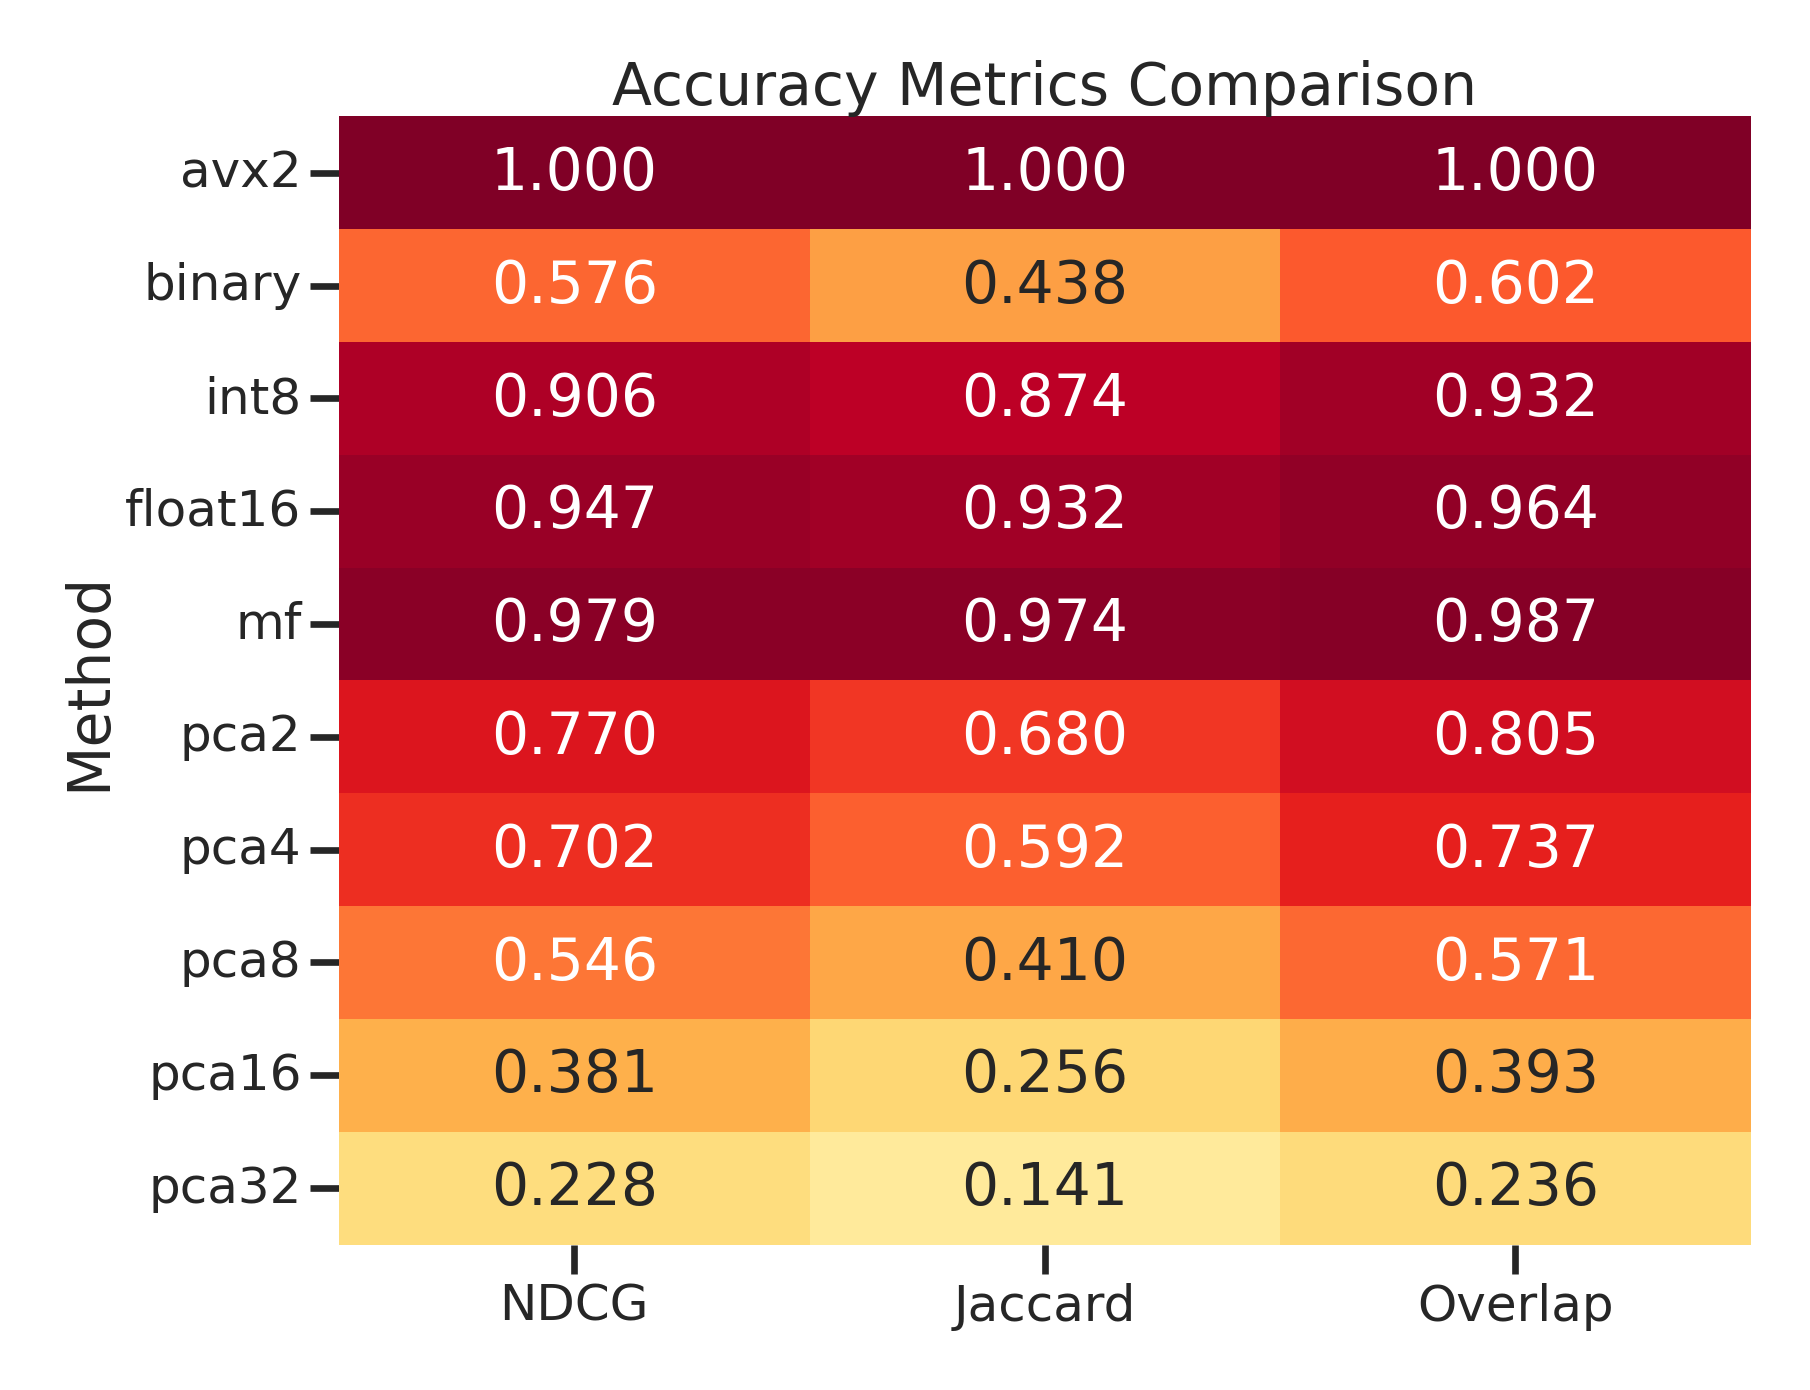
\includegraphics[scale=1]{bilder/plots/accuracy_heatmap_dim1024_k100_q.png}
            %\vspace*{-1cm}
            \caption{Accuracy of searchers}
            \label{accuracyheatmapone}
        \end{minipage}
        %\hfill
        \begin{minipage}{0.49\widefigwidth}
            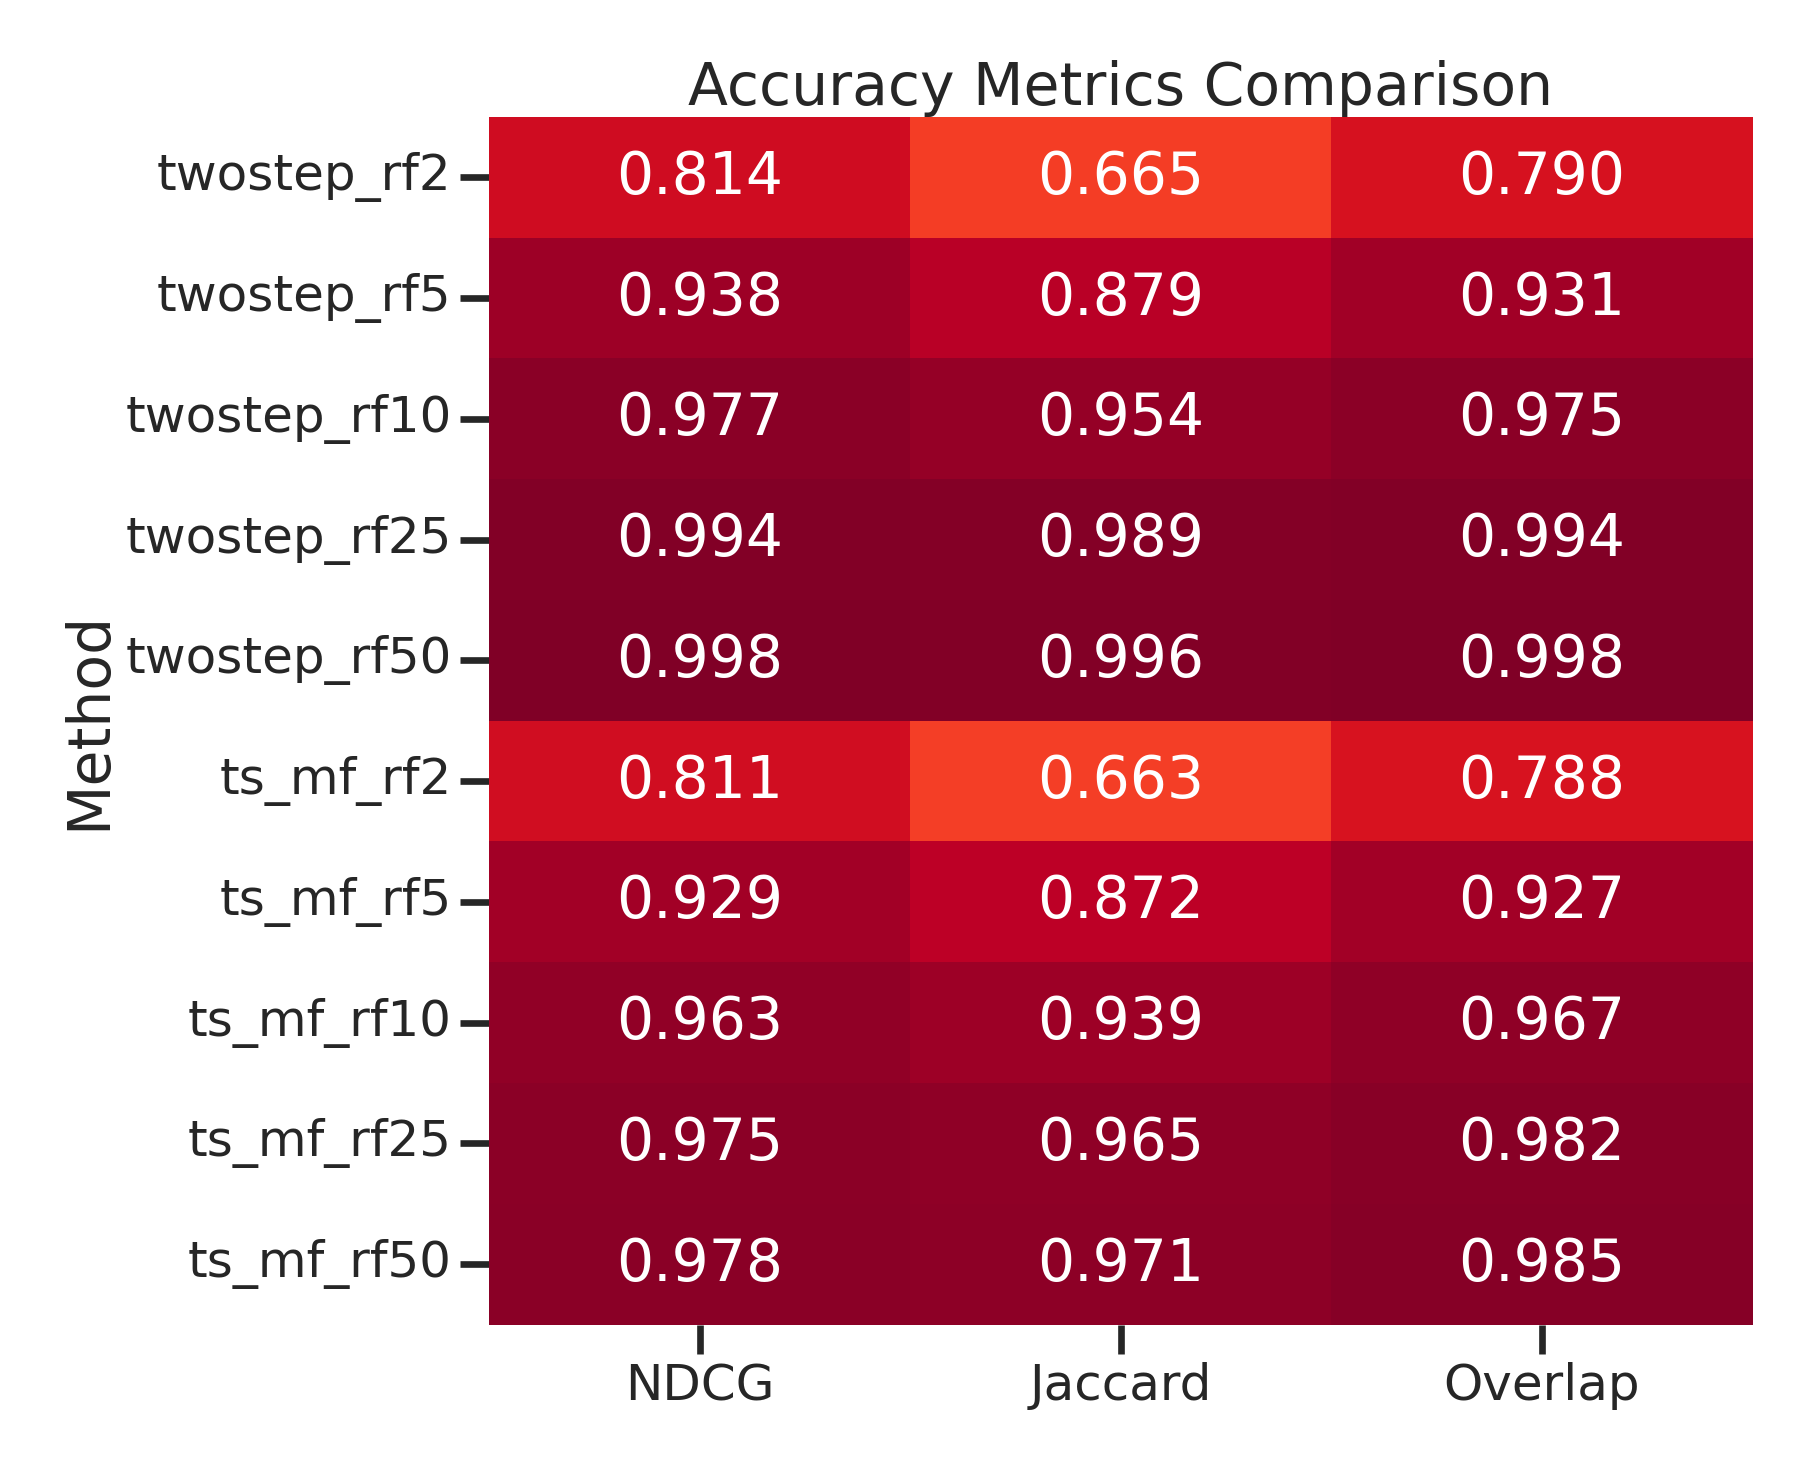
\includegraphics[scale=1]{bilder/plots/accuracy_heatmap_dim1024_k100_q_twostep.png}
            %\vspace*{-1cm}
            \caption{Accuracy of two-step searchers}
            \label{accuracyheatmaptwo}
        \end{minipage}
    }
\end{figure}

\begin{figure}[h]
    \makebox[\textwidth][c]{%
        \begin{minipage}{0.49\widefigwidth}
            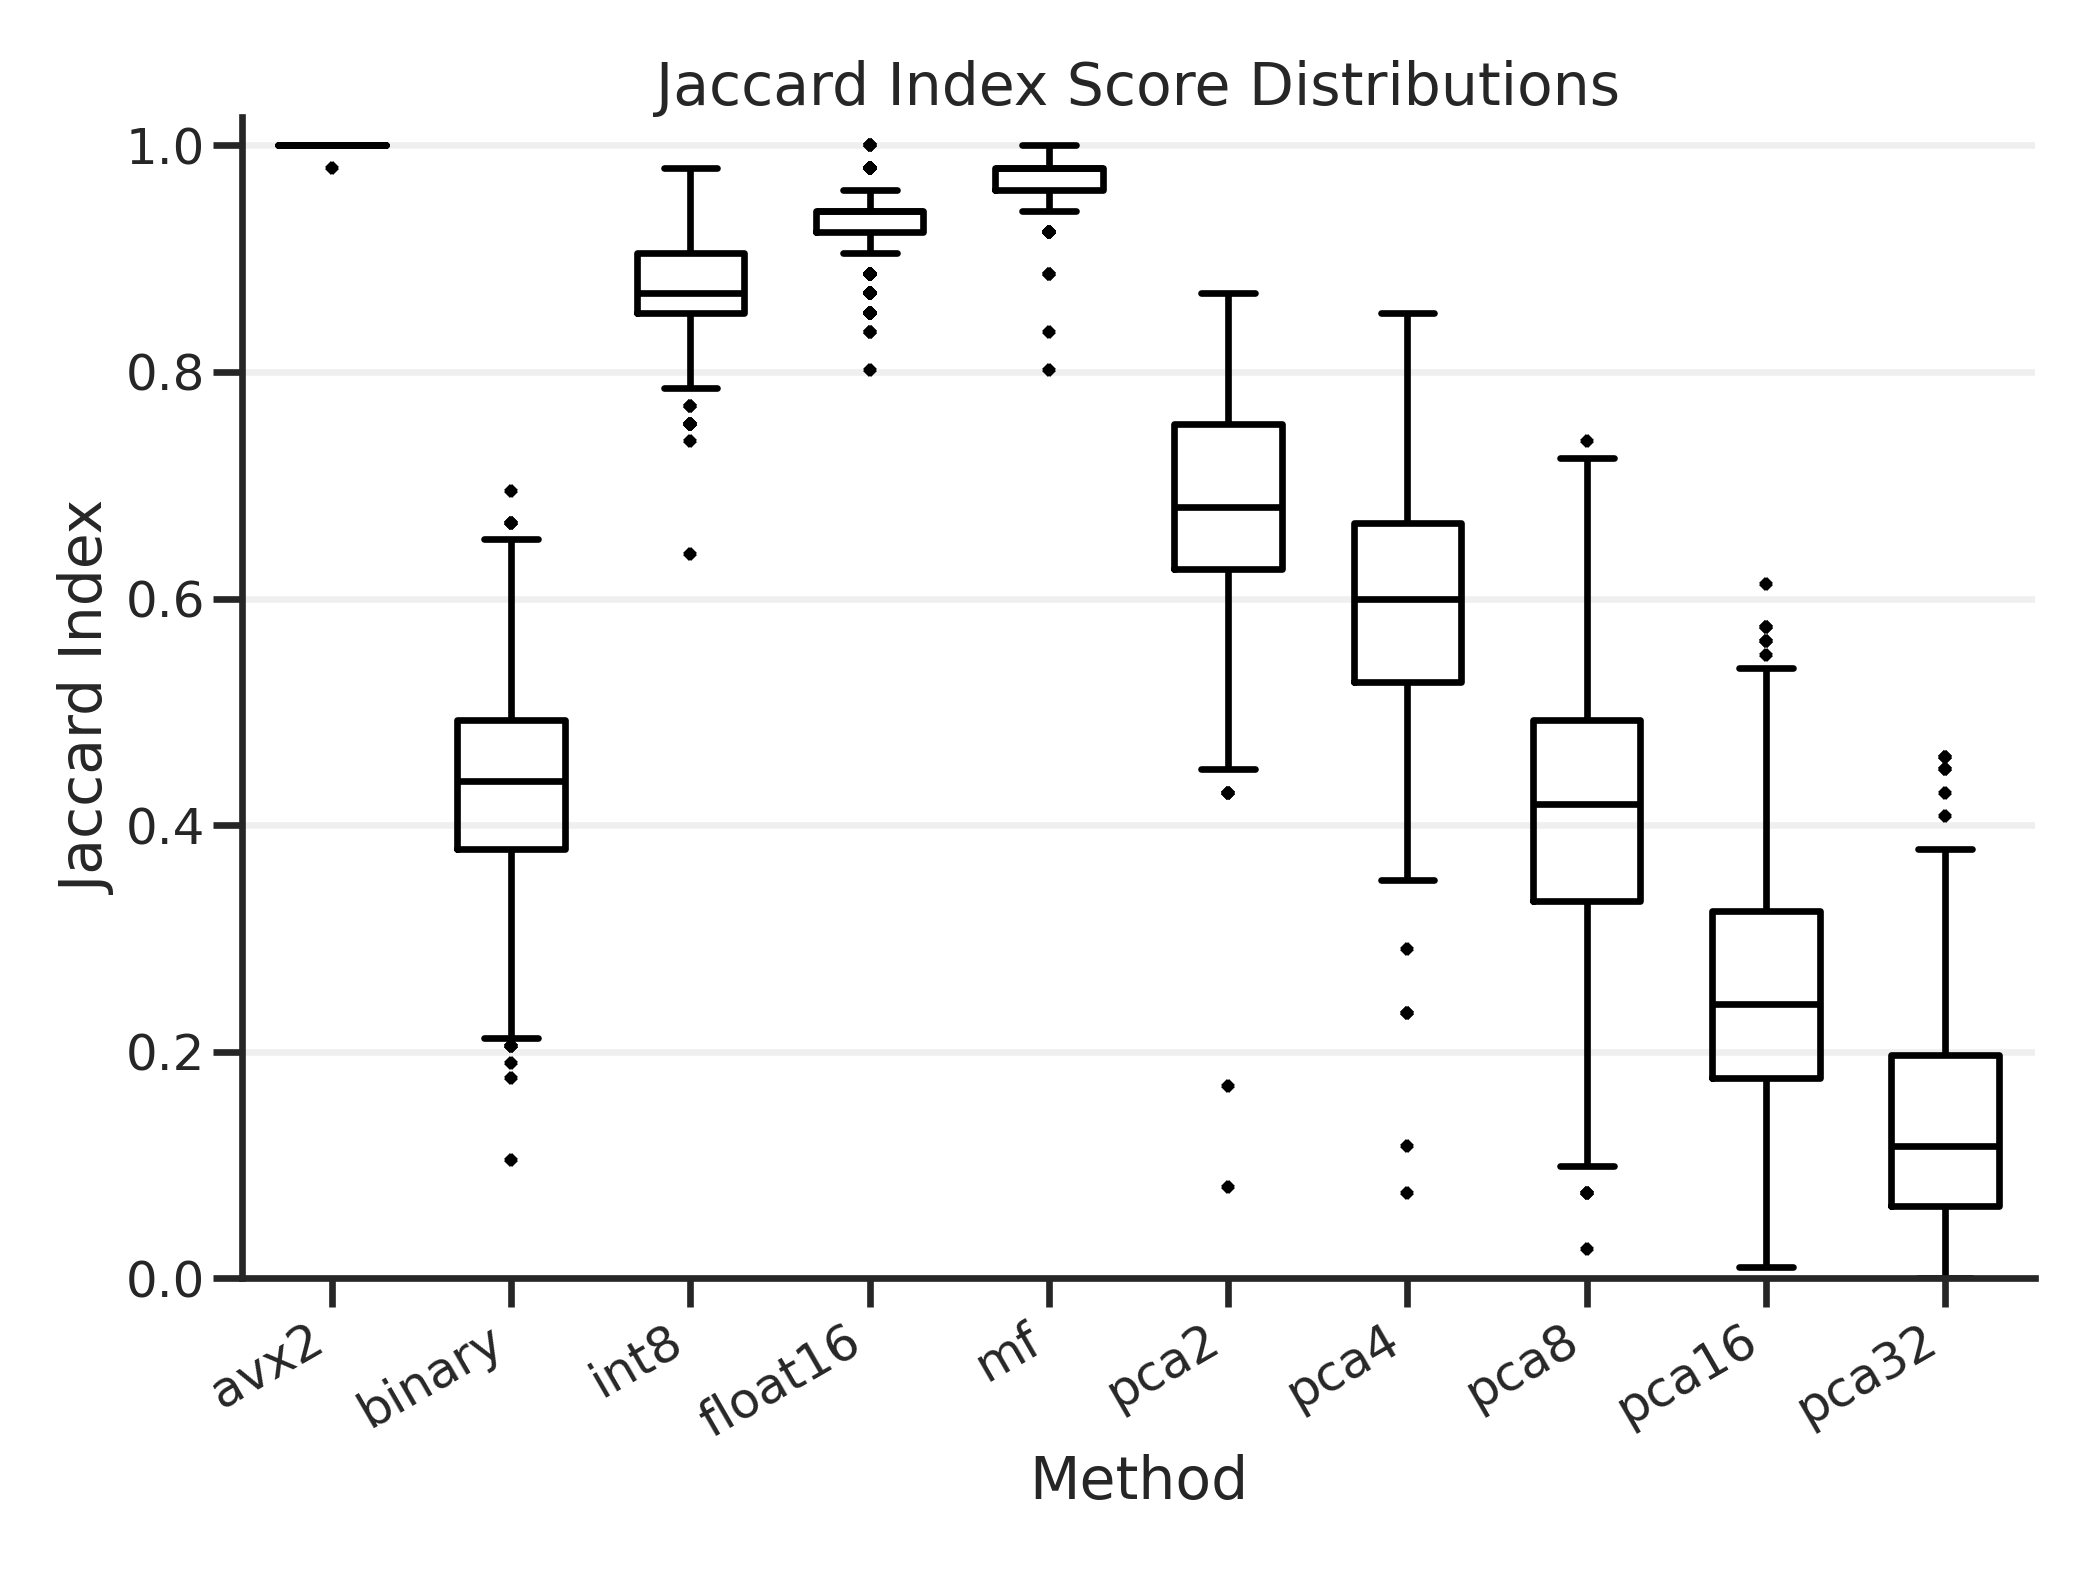
\includegraphics[width=0.49\widefigwidth]{bilder/plots/jaccard_boxplots_dim1024_k100_q.png}
            \vspace*{-1cm}
            \caption{Jaccard index of searchers}
            \label{boxjaccardsearchersone}
        \end{minipage}
        %\hfill
        \begin{minipage}{0.49\widefigwidth}
            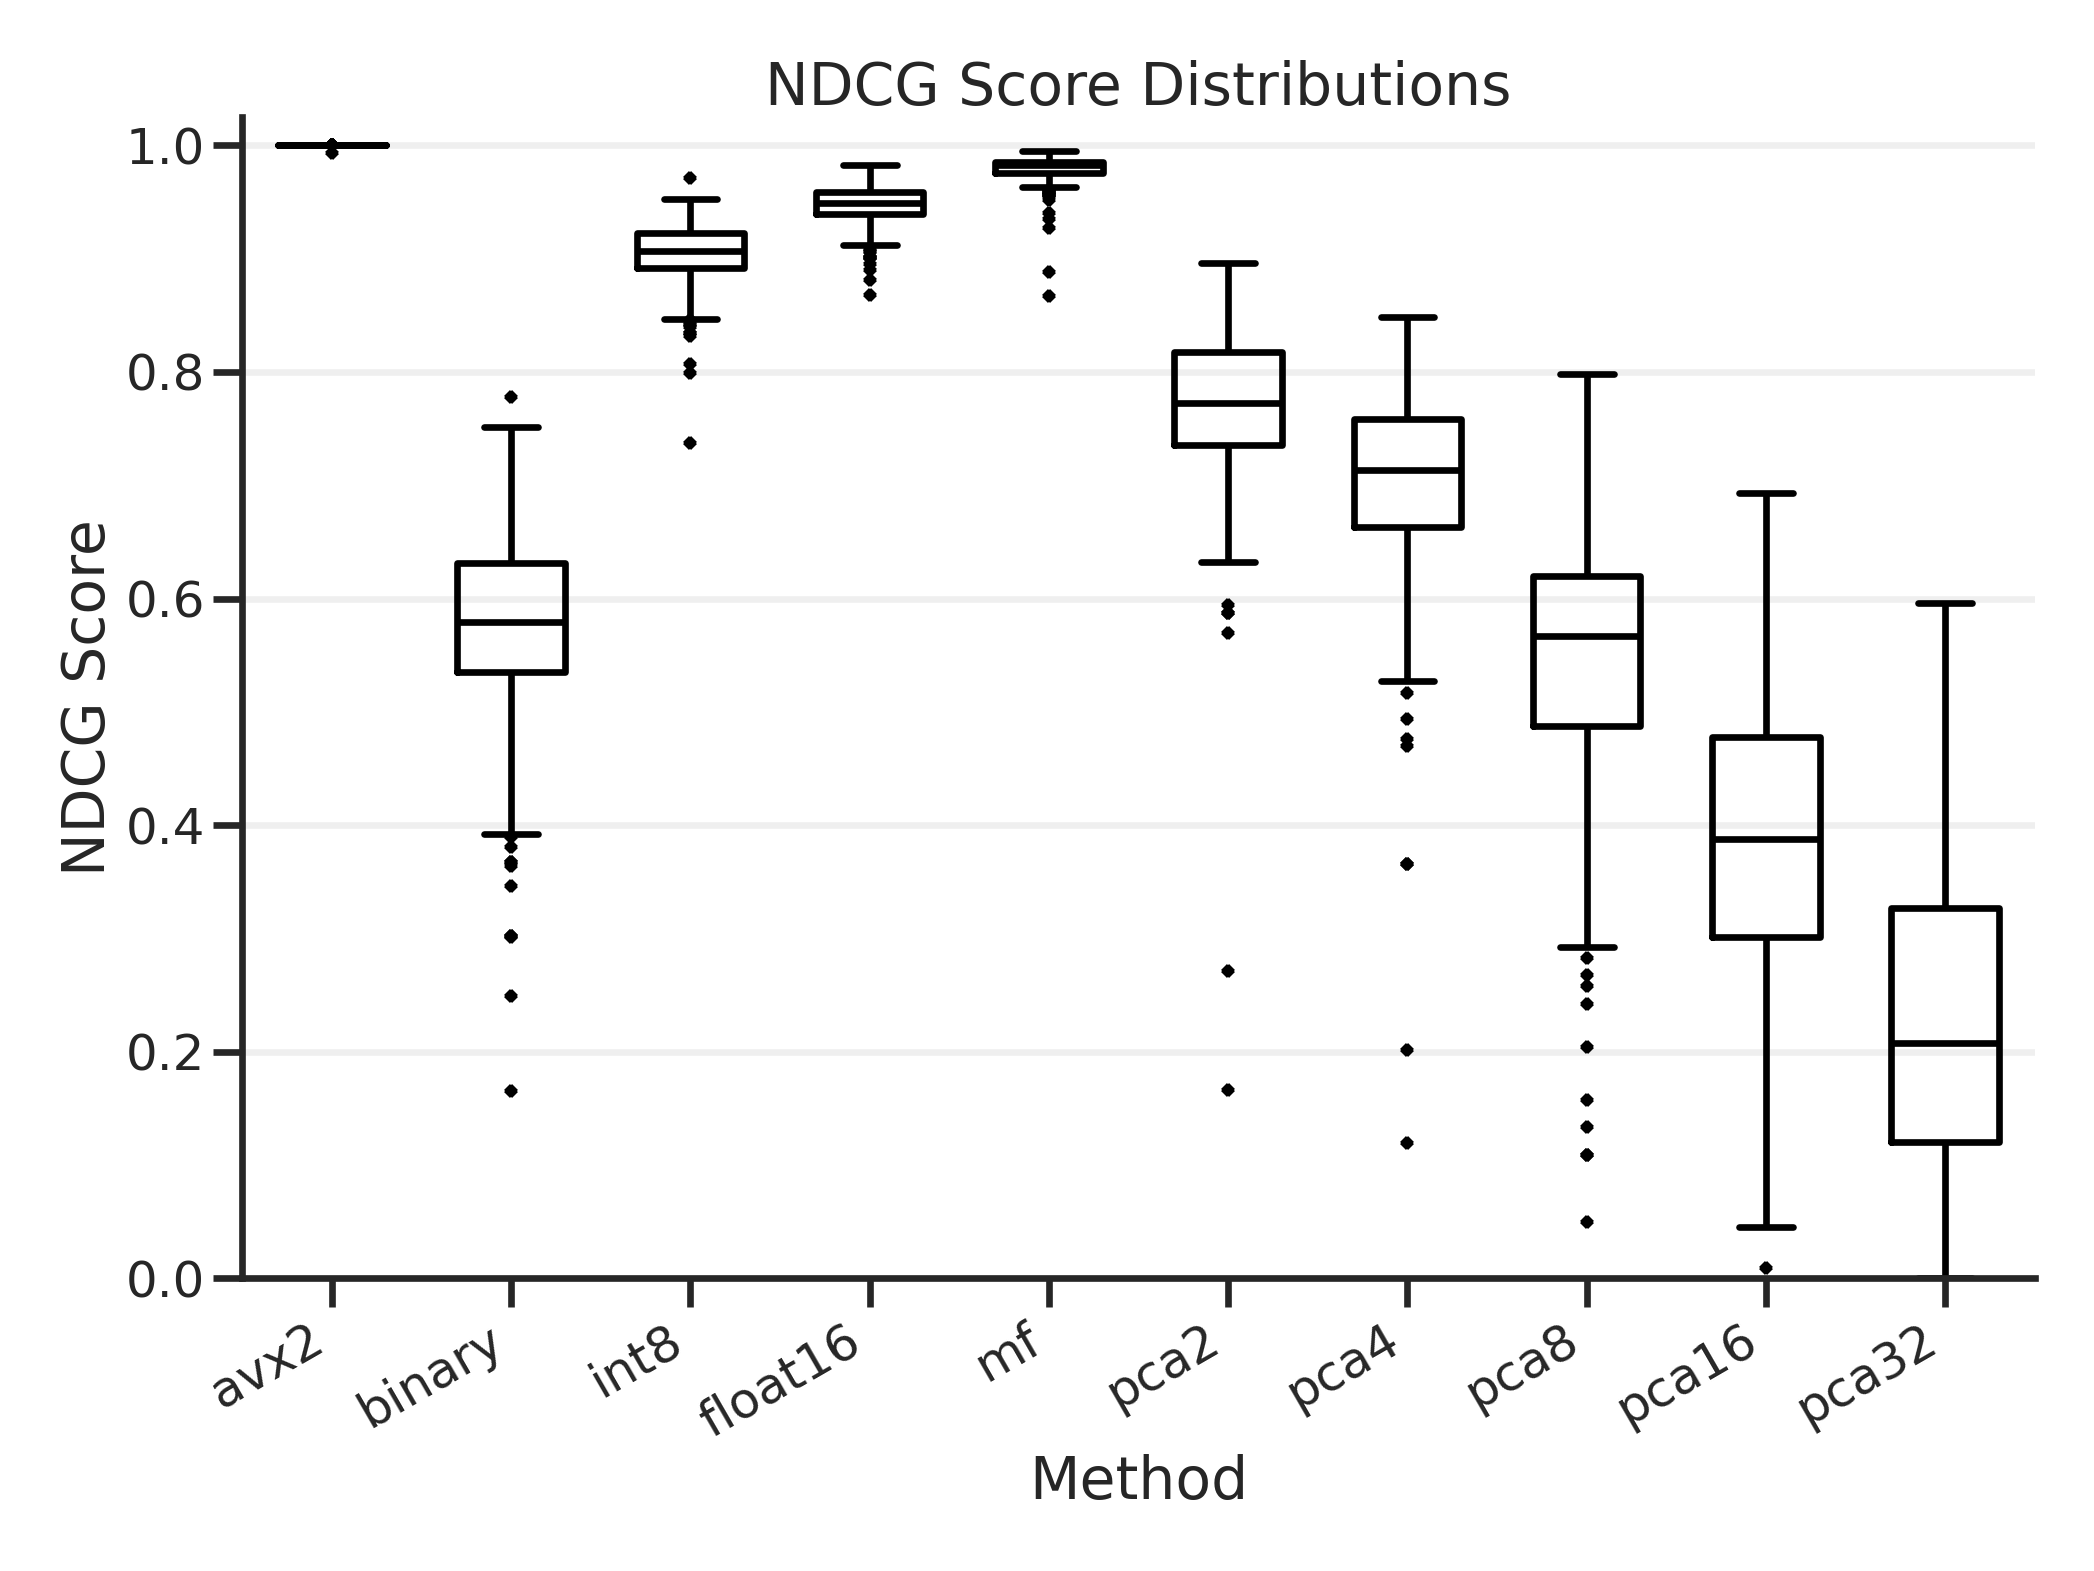
\includegraphics[width=0.49\widefigwidth]{bilder/plots/ndcg_boxplots_dim1024_k100_q.png}
            \vspace*{-1cm}
            \caption{NDCG score of searchers}
            \label{boxndcgsearchersone}
        \end{minipage}
    }
\end{figure}

The binary searcher performs decent with an average NDCG of 0.576 and Jaccard index of 0.438 when considering its heavy quantization, the fast search time and low memory usage. The PCA32 method, for example, uses the same amount of memory but has a much lower score which makes it useless in comparison to the binary searcher. The NDCG being higher than the Jaccard index indicates that the binary searcher also retrieves the important documents quiet reliably. In the box plots in \autoref{boxjaccardsearchersone} and \autoref{boxndcgsearchersone} show some outliers close to, and below 0.2 Jaccard index and slightly above 0.2 NDCG. This means that for some queries it can be unreliable on its own.


The int8 based searcher performs well with an average NDCG of 0.9 and Jaccard index of 0.87. It performs exclusively above the binary searcher. The outliers are also a lot less drastic. Especially the NDCG stays above 0.8 for all queries except one.

Float16 or half precision float has very good average accuracy scores \autoref{accuracyheatmapone}. The box plots in \autoref{boxjaccardsearchersone} and \autoref{boxndcgsearchersone} also show it performing very good. Especially the first and third quartile have a very close range and stay above 0.92 Jaccard index and 0.94 NDCG. The outliers are also still very good with at least 0.8 Jaccard index and 0.87 NDCG. This makes it suitable to fully replace the float32 approach as it gives good memory savings, reliable results and is much faster on supported hardware.

Even better performs the mapped float searcher. On average, it gets close to perfect scores (\autoref{accuracyheatmapone}). The outliers are no worse than the float16 outliers and the lower percentiles are above 0.96 for both metrics. This makes it the most accurate quantization tested.

The variants with PCA dimension reduction applied to the embeddings mostly perform worse than methods with the similar memory usage and search speed. Int8 is more accurate than PCA2 and only uses half the memory, while PCA2 only got a slight speed advantage. When comparing it to the binary search method, we see, that PCA8 performs worse while taking 3 times longer and using quadruple the memory. The bad performance when using PCA for embeddings is also mentioned here.~\cite{thakur2023injectingdomainadaptationlearningtohash}

\begin{figure}[h]
    \makebox[\textwidth][c]{%
        \begin{minipage}{0.49\widefigwidth}
            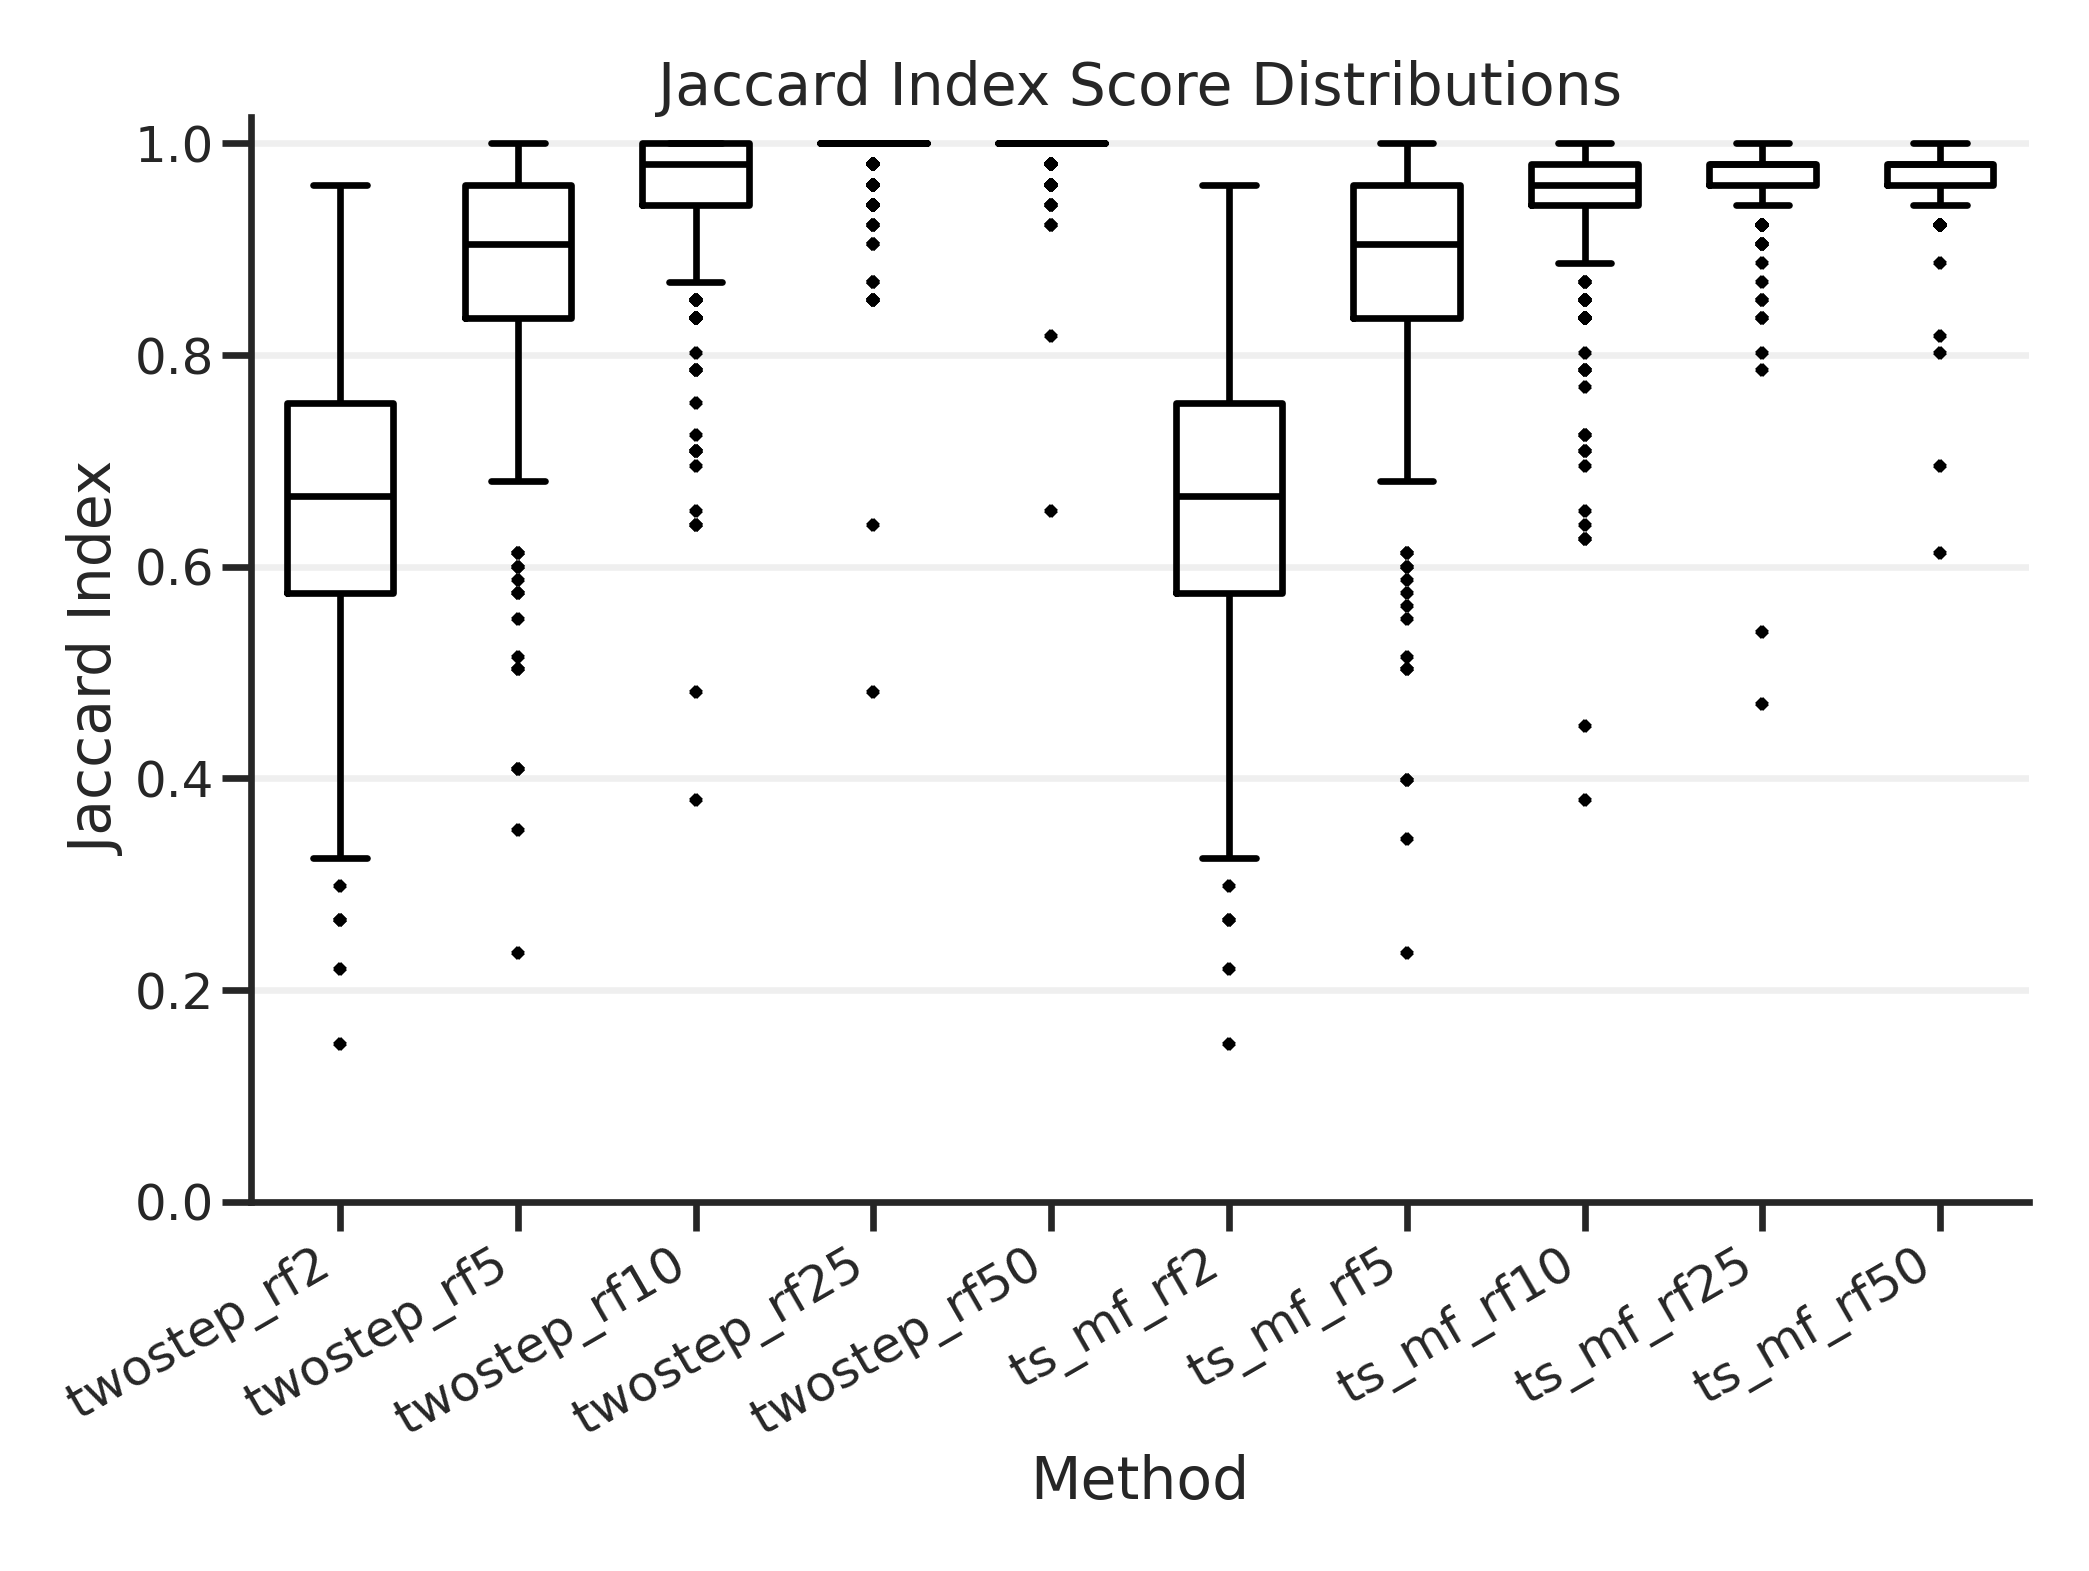
\includegraphics[width=0.49\widefigwidth]{bilder/plots/jaccard_boxplots_dim1024_k100_q_twostep.png}
            \vspace*{-1cm}
            \caption{Jaccard index of two-step searchers}
            \label{boxjaccardsearcherstwo}
        \end{minipage}
        %\hfill
        \begin{minipage}{0.49\widefigwidth}
            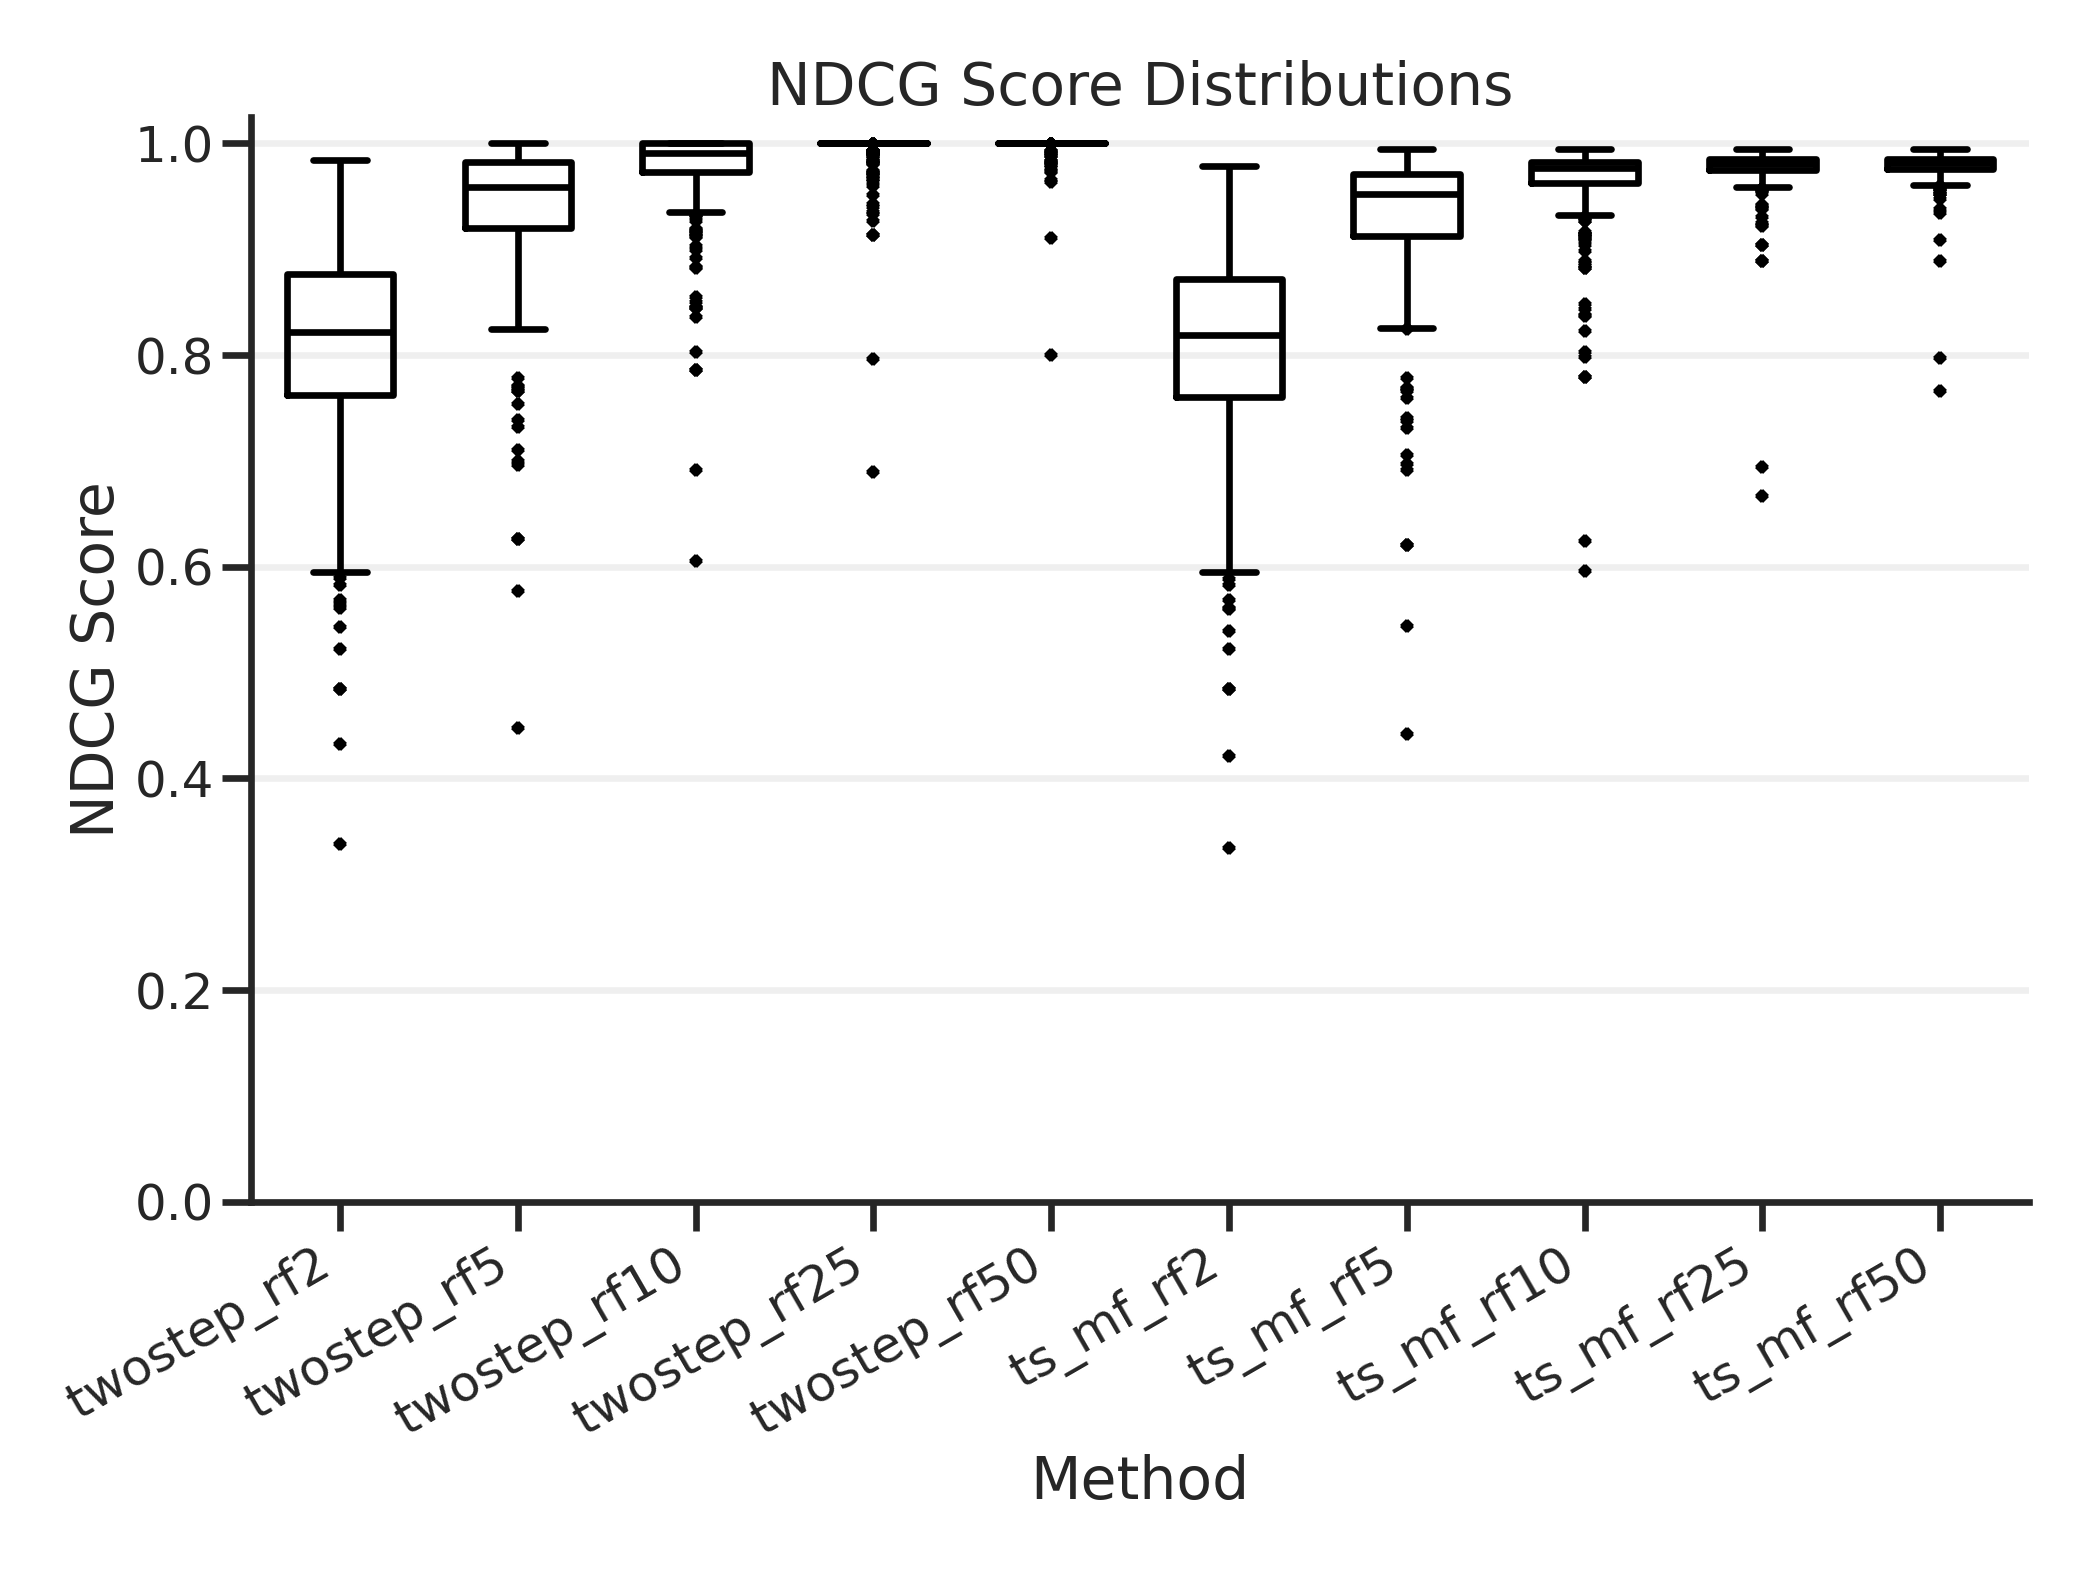
\includegraphics[width=0.49\widefigwidth]{bilder/plots/ndcg_boxplots_dim1024_k100_q_twostep.png}
            \vspace*{-1cm}
            \caption{NDCG score of two-step searchers}
            \label{boxndcgsearcherstwo}
        \end{minipage}
    }
\end{figure}

Both two-step methods (binary+float and binary+mapped float) perform really well. Especially with rescoring factors of 10 and higher. For a rescoring factor of 10 they have a first quartile NDCG score of 0.96 and 0.97 respectively. The outliers from the binary searcher still exists and only get slightly better as the rescoring factor increases.
With a rescoring factor of 25 or higher the binary+float searcher mostly gets perfect scores, except for the outliers. The score for the binary+mapped float searcher is capped by the mapped float searcher which is still very high.

\subsection{Accuracy vs Rescoring Factor}

As mentioned in the previous section the search time increases when increasing the rescoring factor. The increase in time is linear as seen in \autoref{time_ndcg_jaccard_vs_rescoring_factor_bf} and \autoref{time_ndcg_jaccard_vs_rescoring_factor_bmf}. The search time overall stays very low as even with high rescore factors the number of prefiltered embeddings is very small compared to the total number of embeddings. At a rescoring factor of 25 the score is very close to the full search equivalent of the second method. The only point in increasing it further is to reduce outliers.
\begin{figure}[h]
    \makebox[\textwidth][c]{%
        \begin{minipage}[t]{0.49\widefigwidth}
            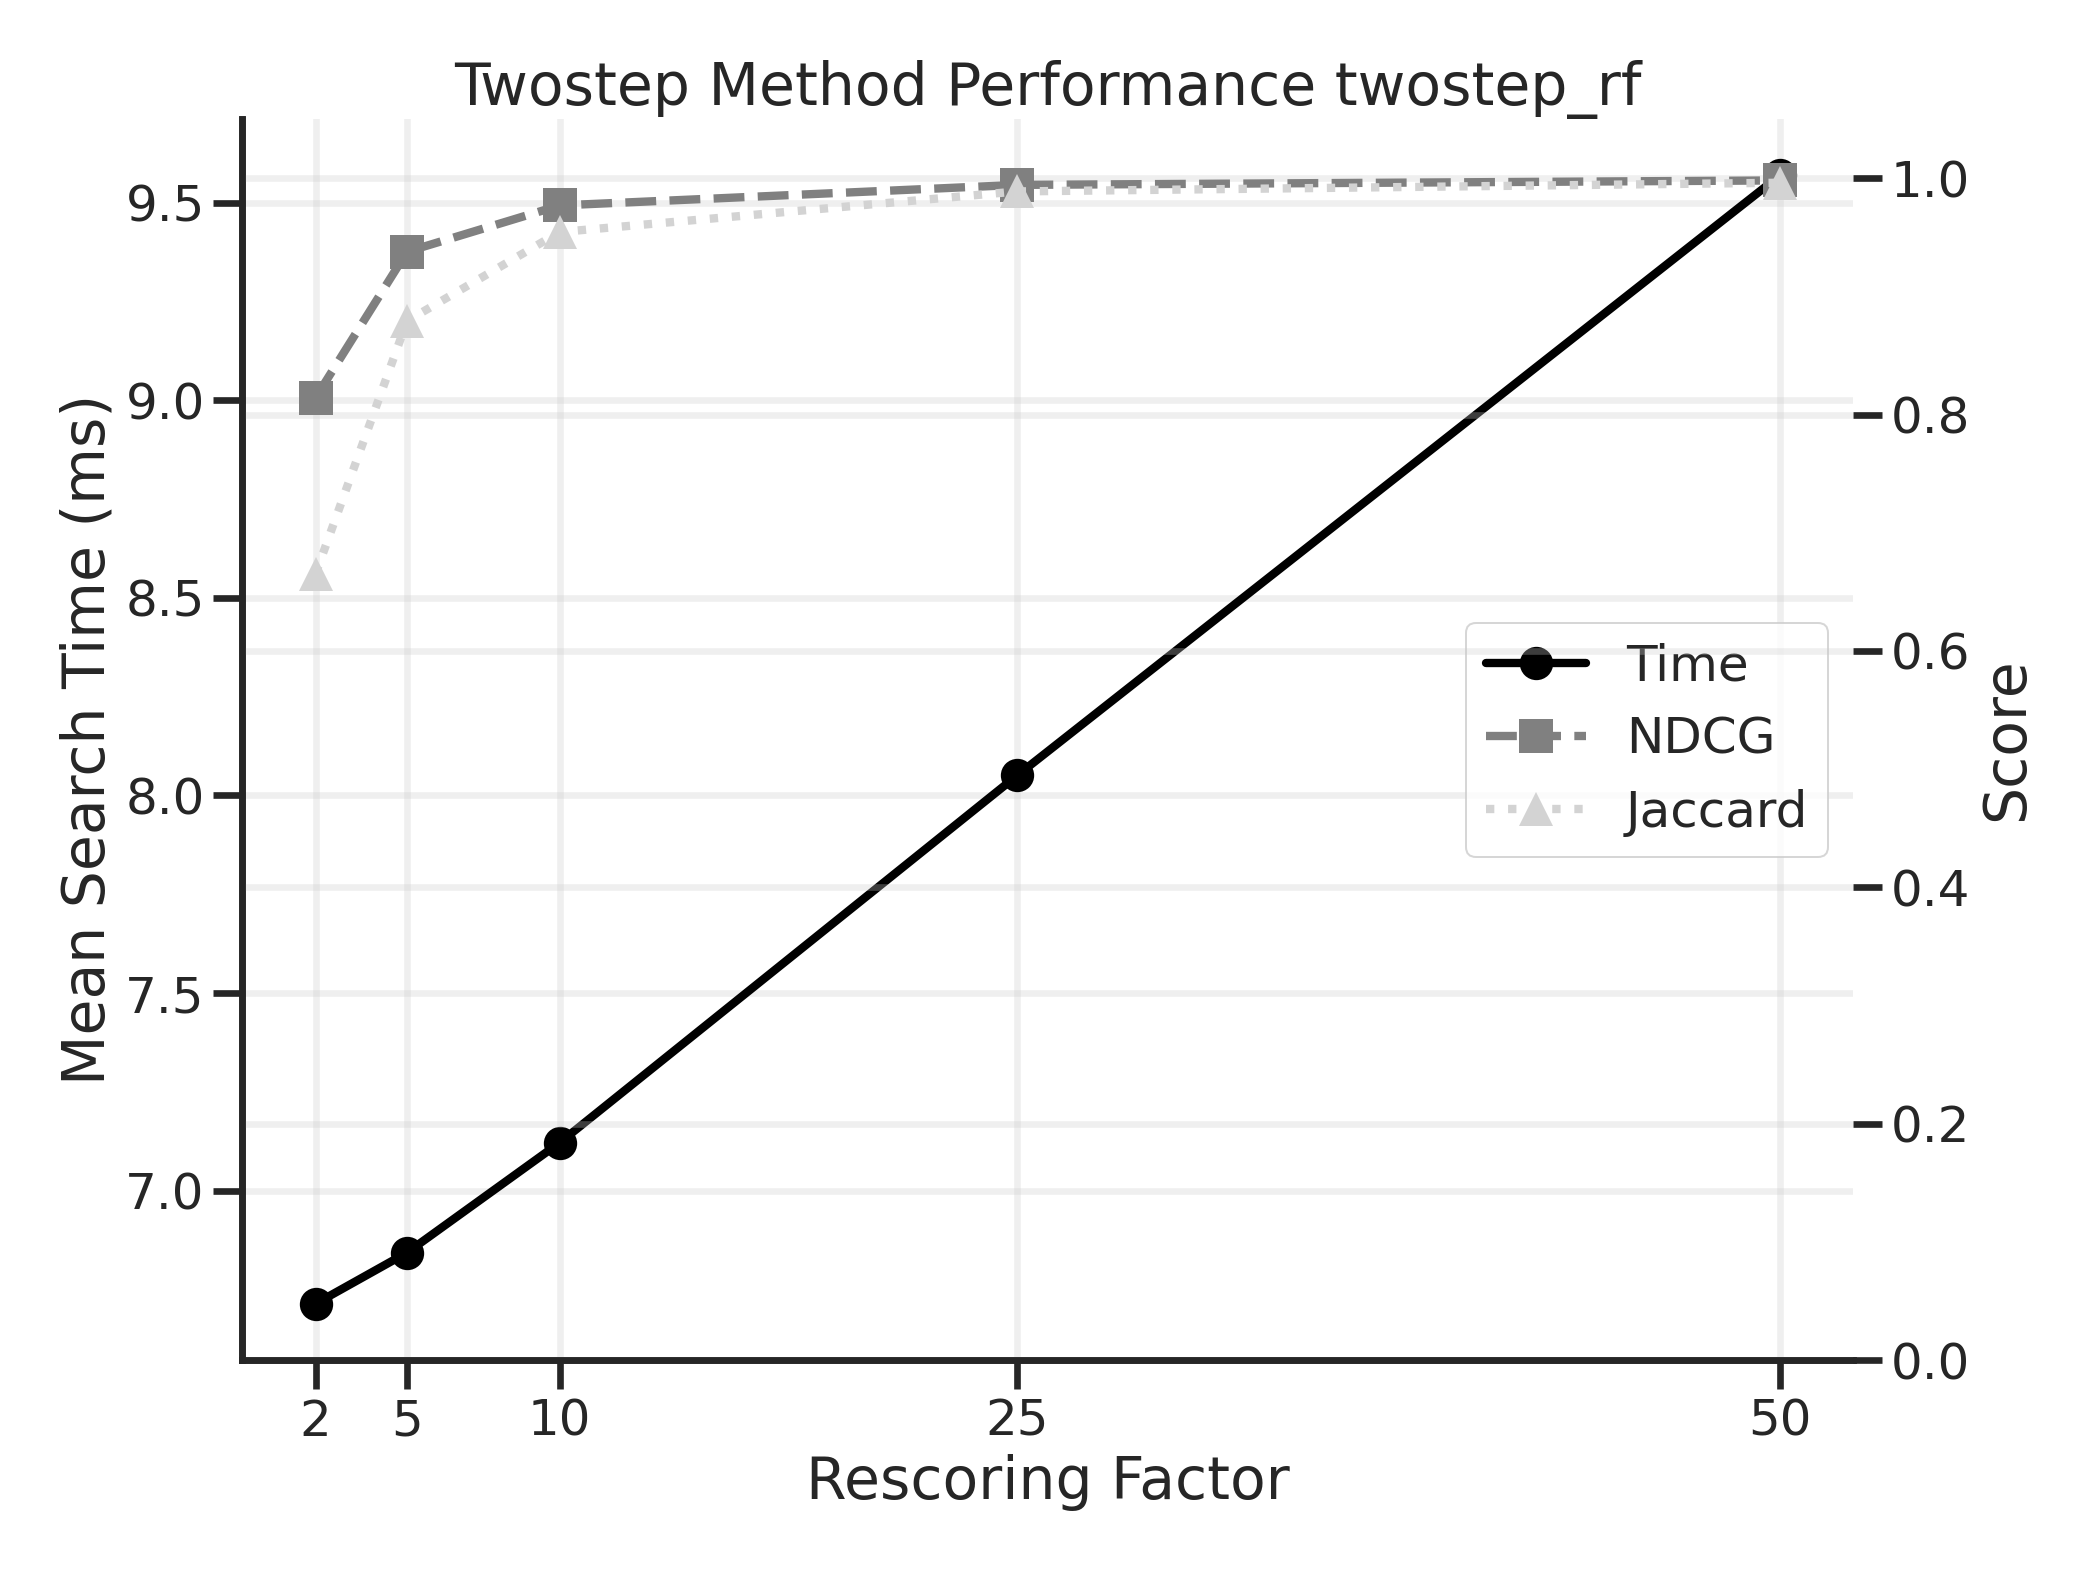
\includegraphics[width=0.49\widefigwidth]{bilder/plots/twostep_comparison_combined_benchmark_dim1024_k100_q.png}
            \vspace*{-1cm}
            \caption{\scriptsize{Time, NDCG, Jaccard vs Rescoring Factor Binary+Float}}
            \label{time_ndcg_jaccard_vs_rescoring_factor_bf}
        \end{minipage}
        %\hfill
        \begin{minipage}[t]{0.49\widefigwidth}
            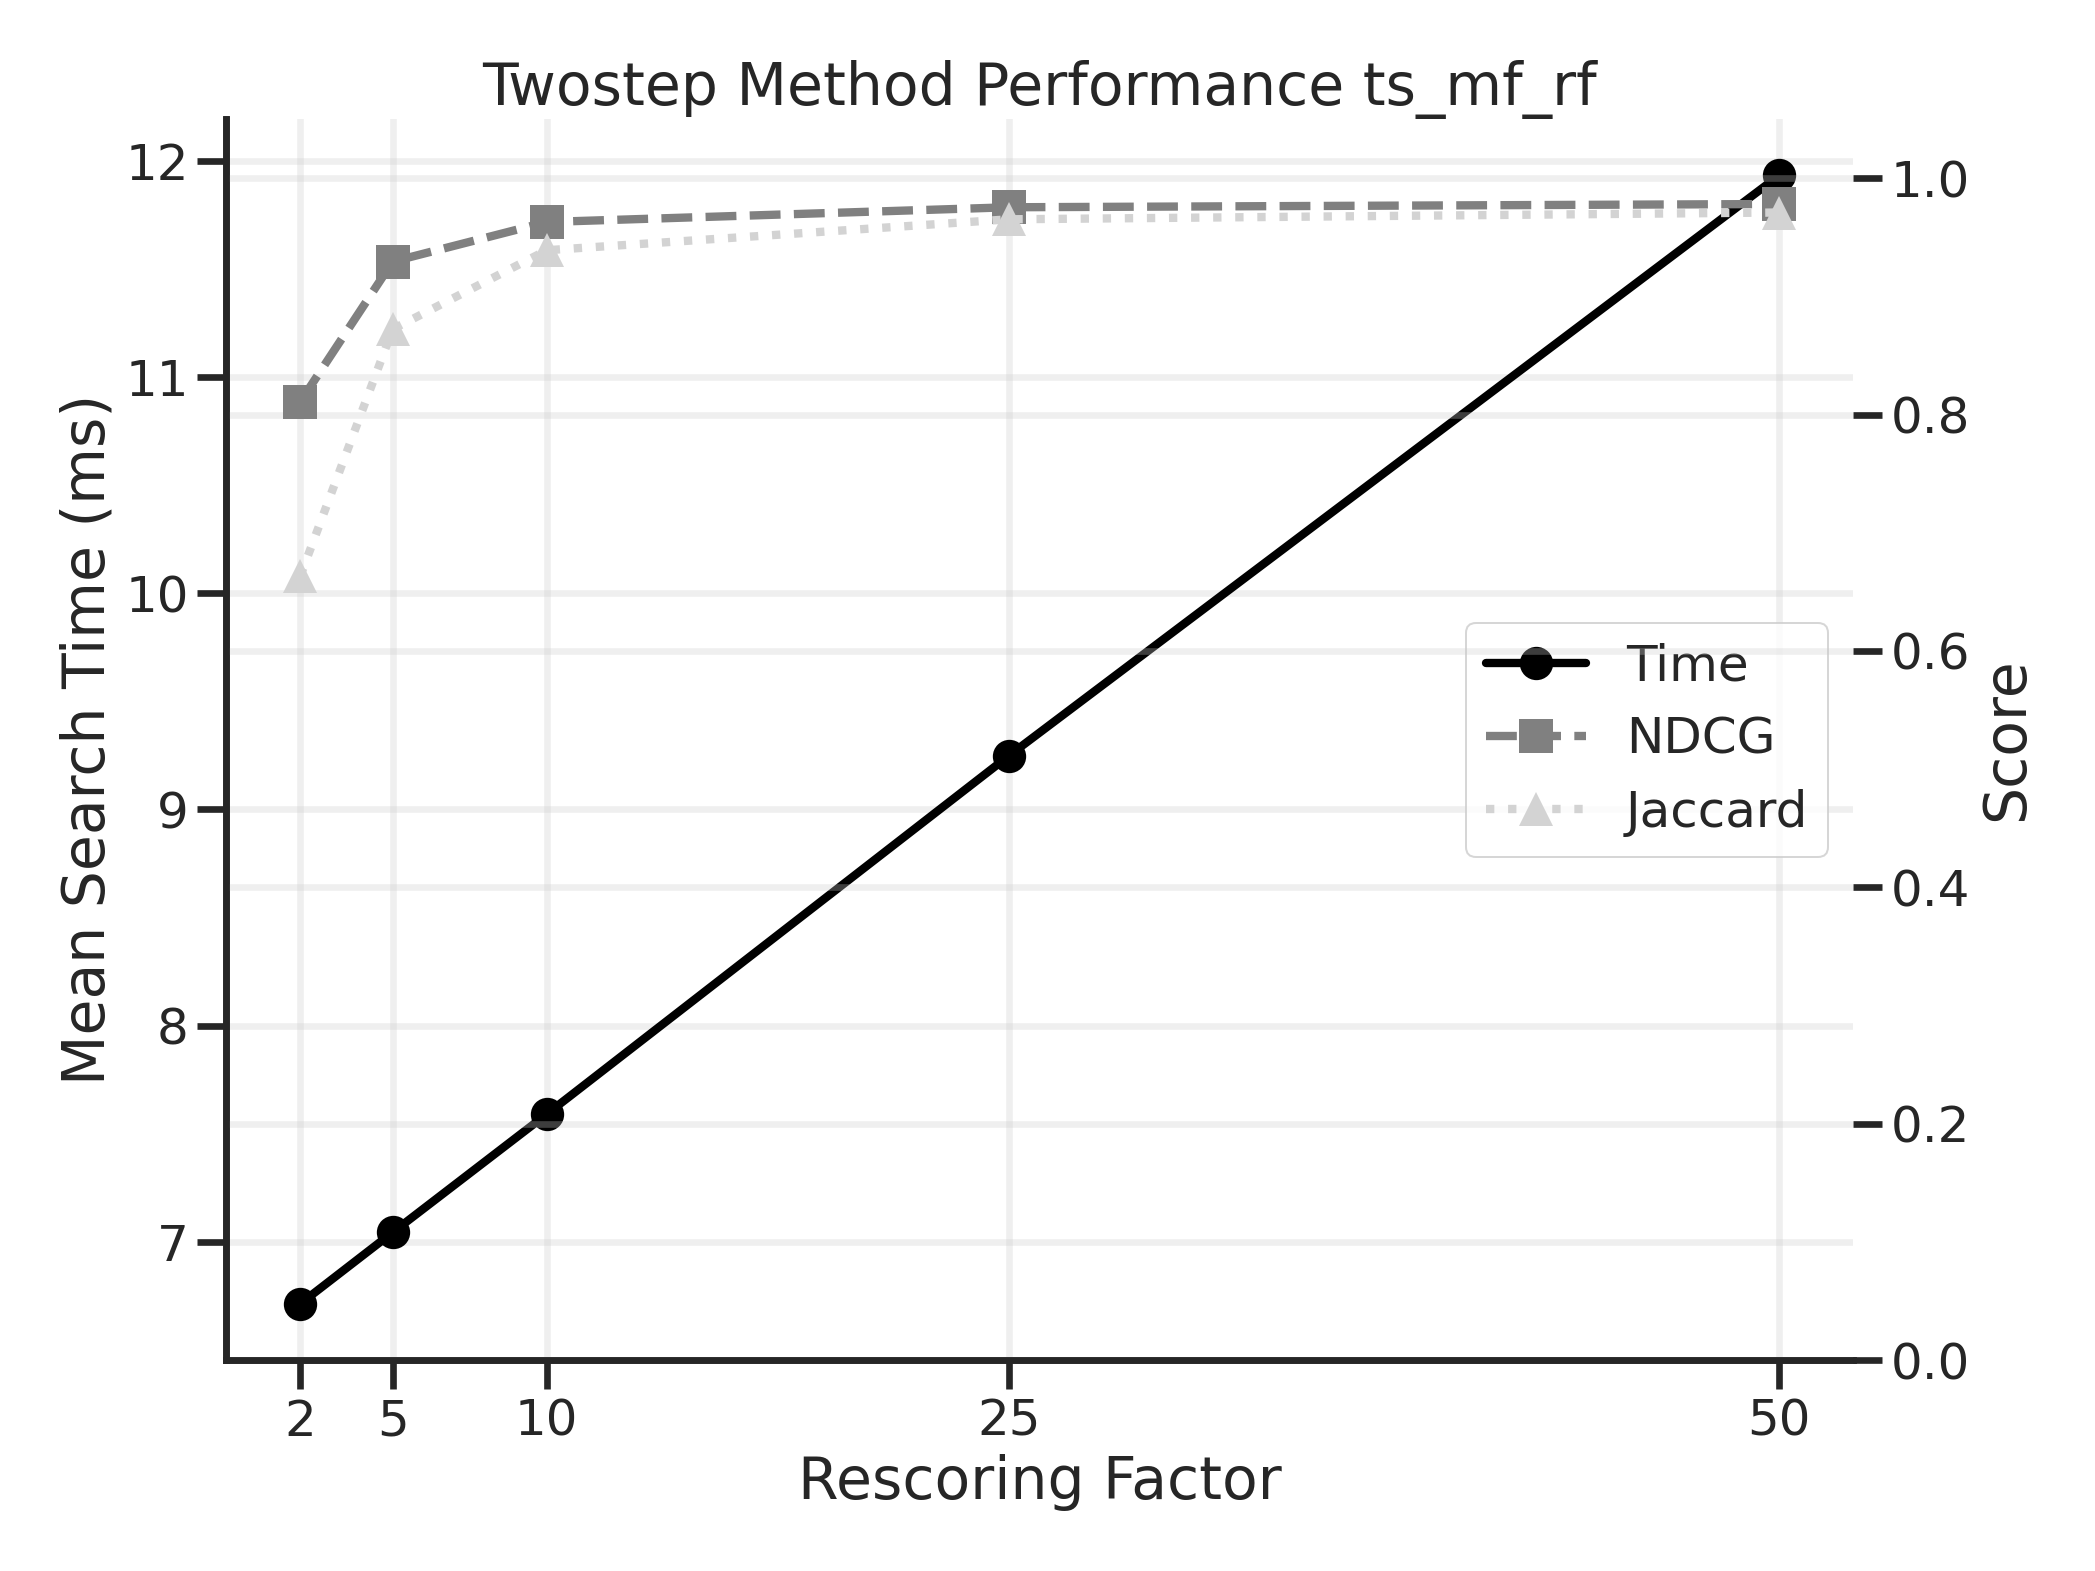
\includegraphics[width=0.49\widefigwidth]{bilder/plots/twostep_comparison_combined_benchmark_dim1024_k100_q_mf.png}
            \vspace*{-1cm}
            \caption{\scriptsize{Time, NDCG, Jaccard vs Rescoring Factor Binary+Mapped Float}}
            \label{time_ndcg_jaccard_vs_rescoring_factor_bmf}
        \end{minipage}
    }
\end{figure}

\subsection{Comparing Benchmark Results from Different Models}
\begin{figure}[h]
    \makebox[\textwidth][c]{%
        \begin{minipage}{0.49\widefigwidth}
            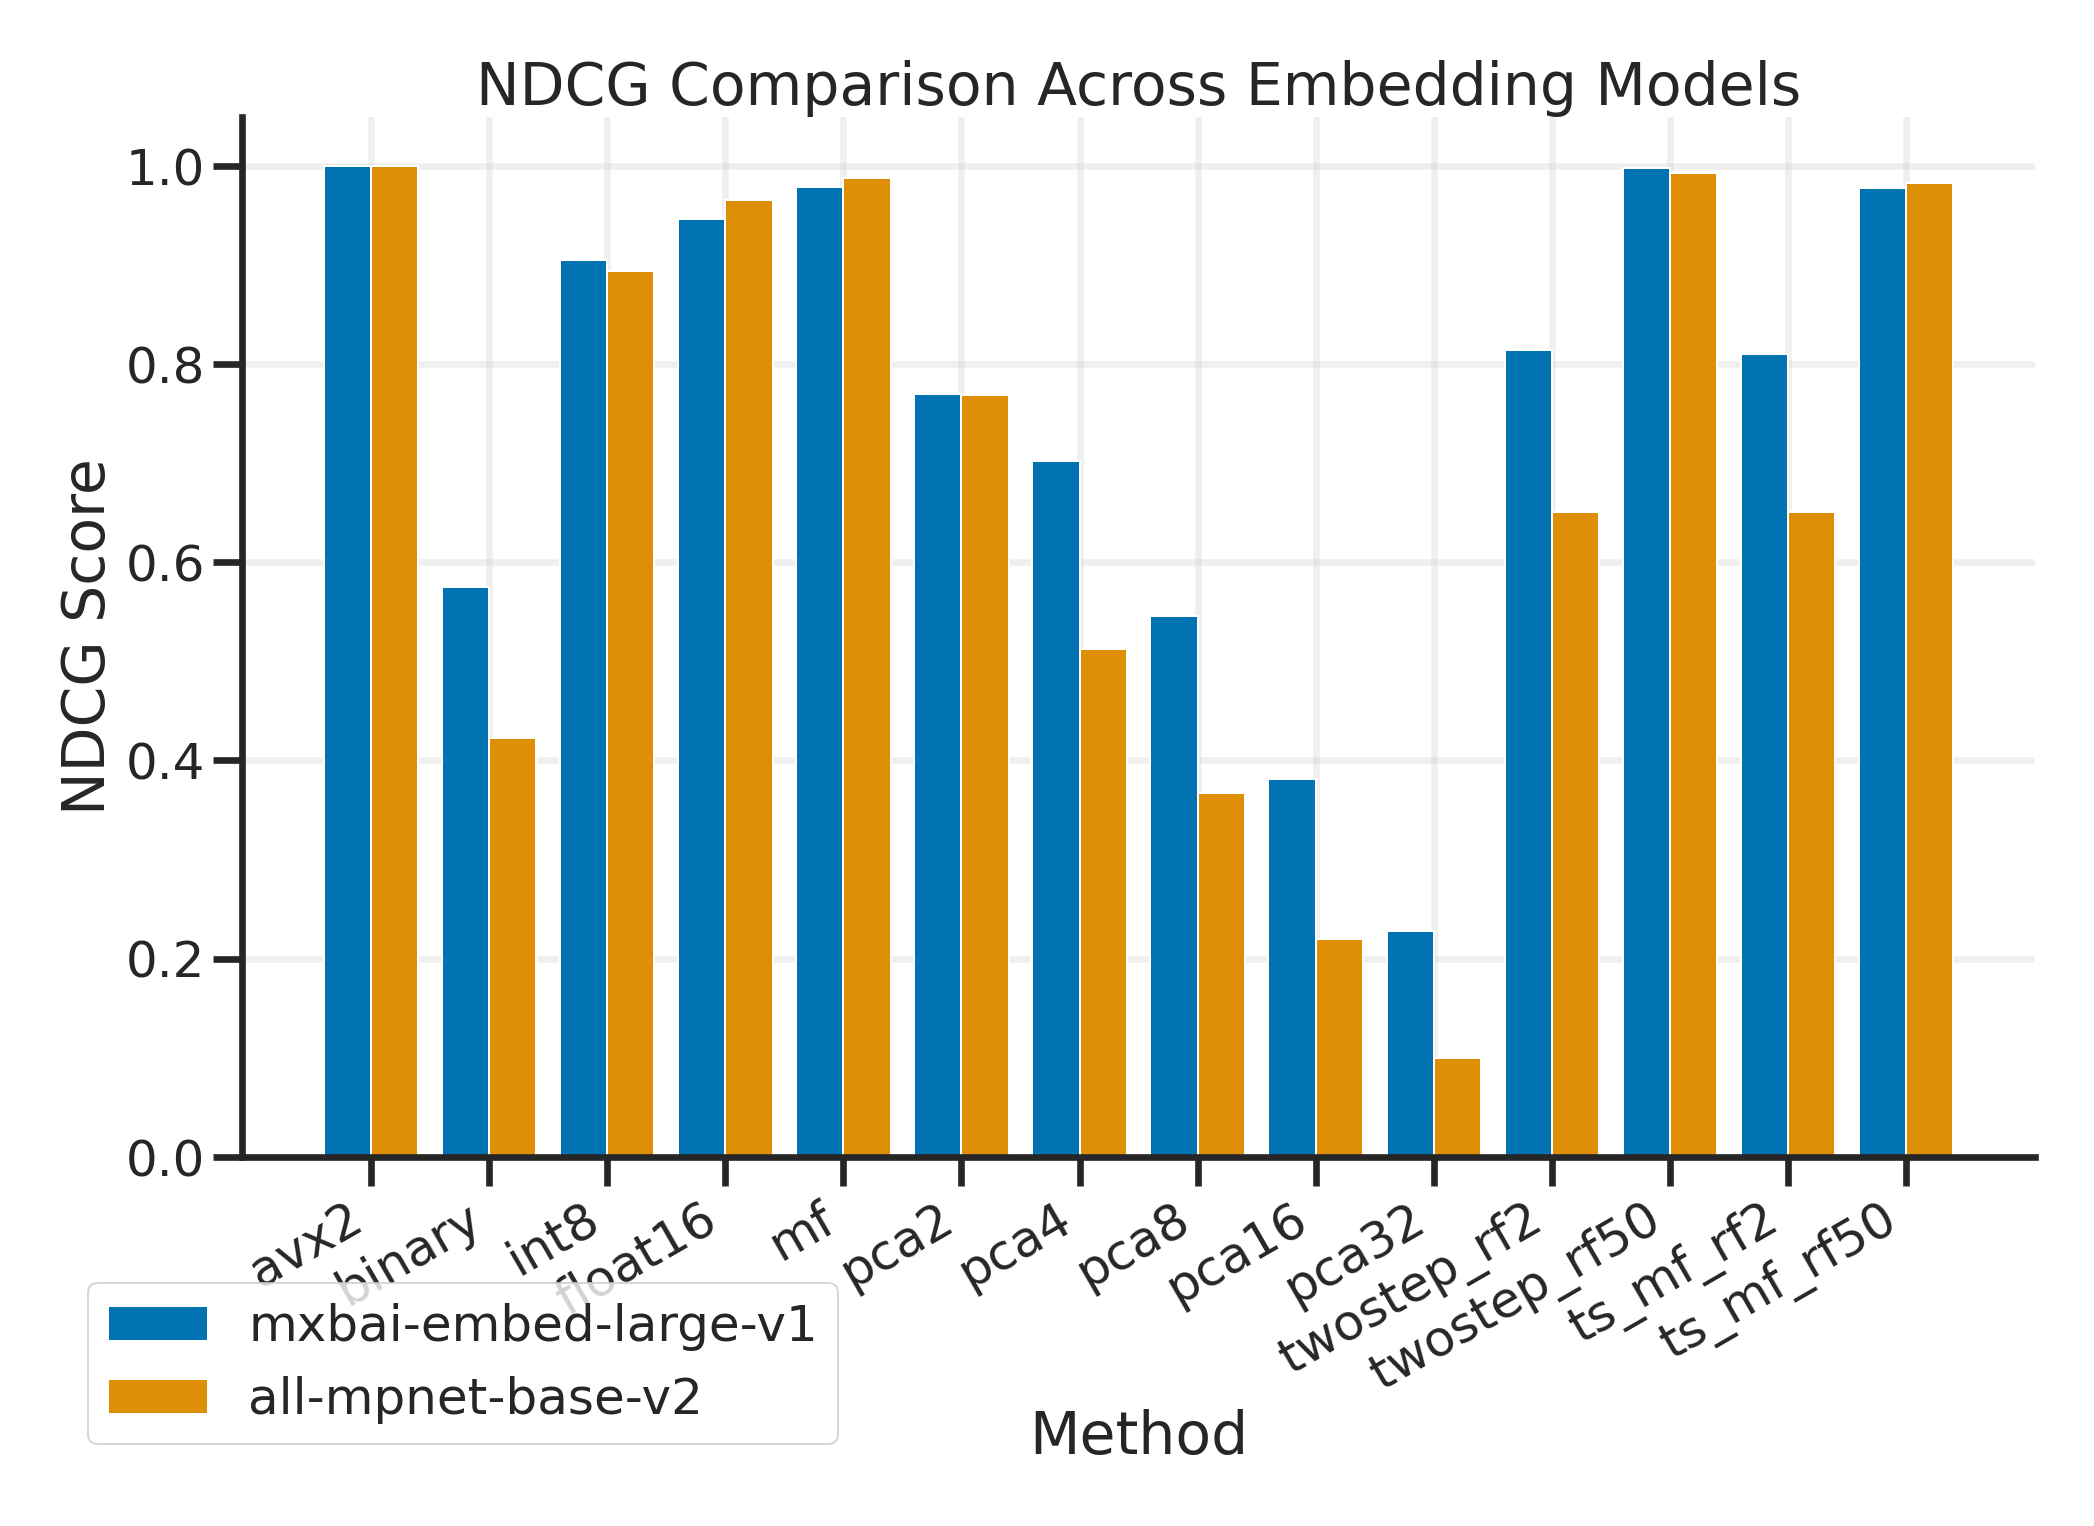
\includegraphics[width=0.49\widefigwidth]{bilder/plots/benchmark_comparison_dim1024_k100_q_dim768_k100_q.png}
            \vspace*{-1cm}
            \caption{\scriptsize{NDCG score comparison between different models}}
            \label{ndcg_comp_diff_models}
        \end{minipage}
        %\hfill
        \begin{minipage}{0.49\widefigwidth}
            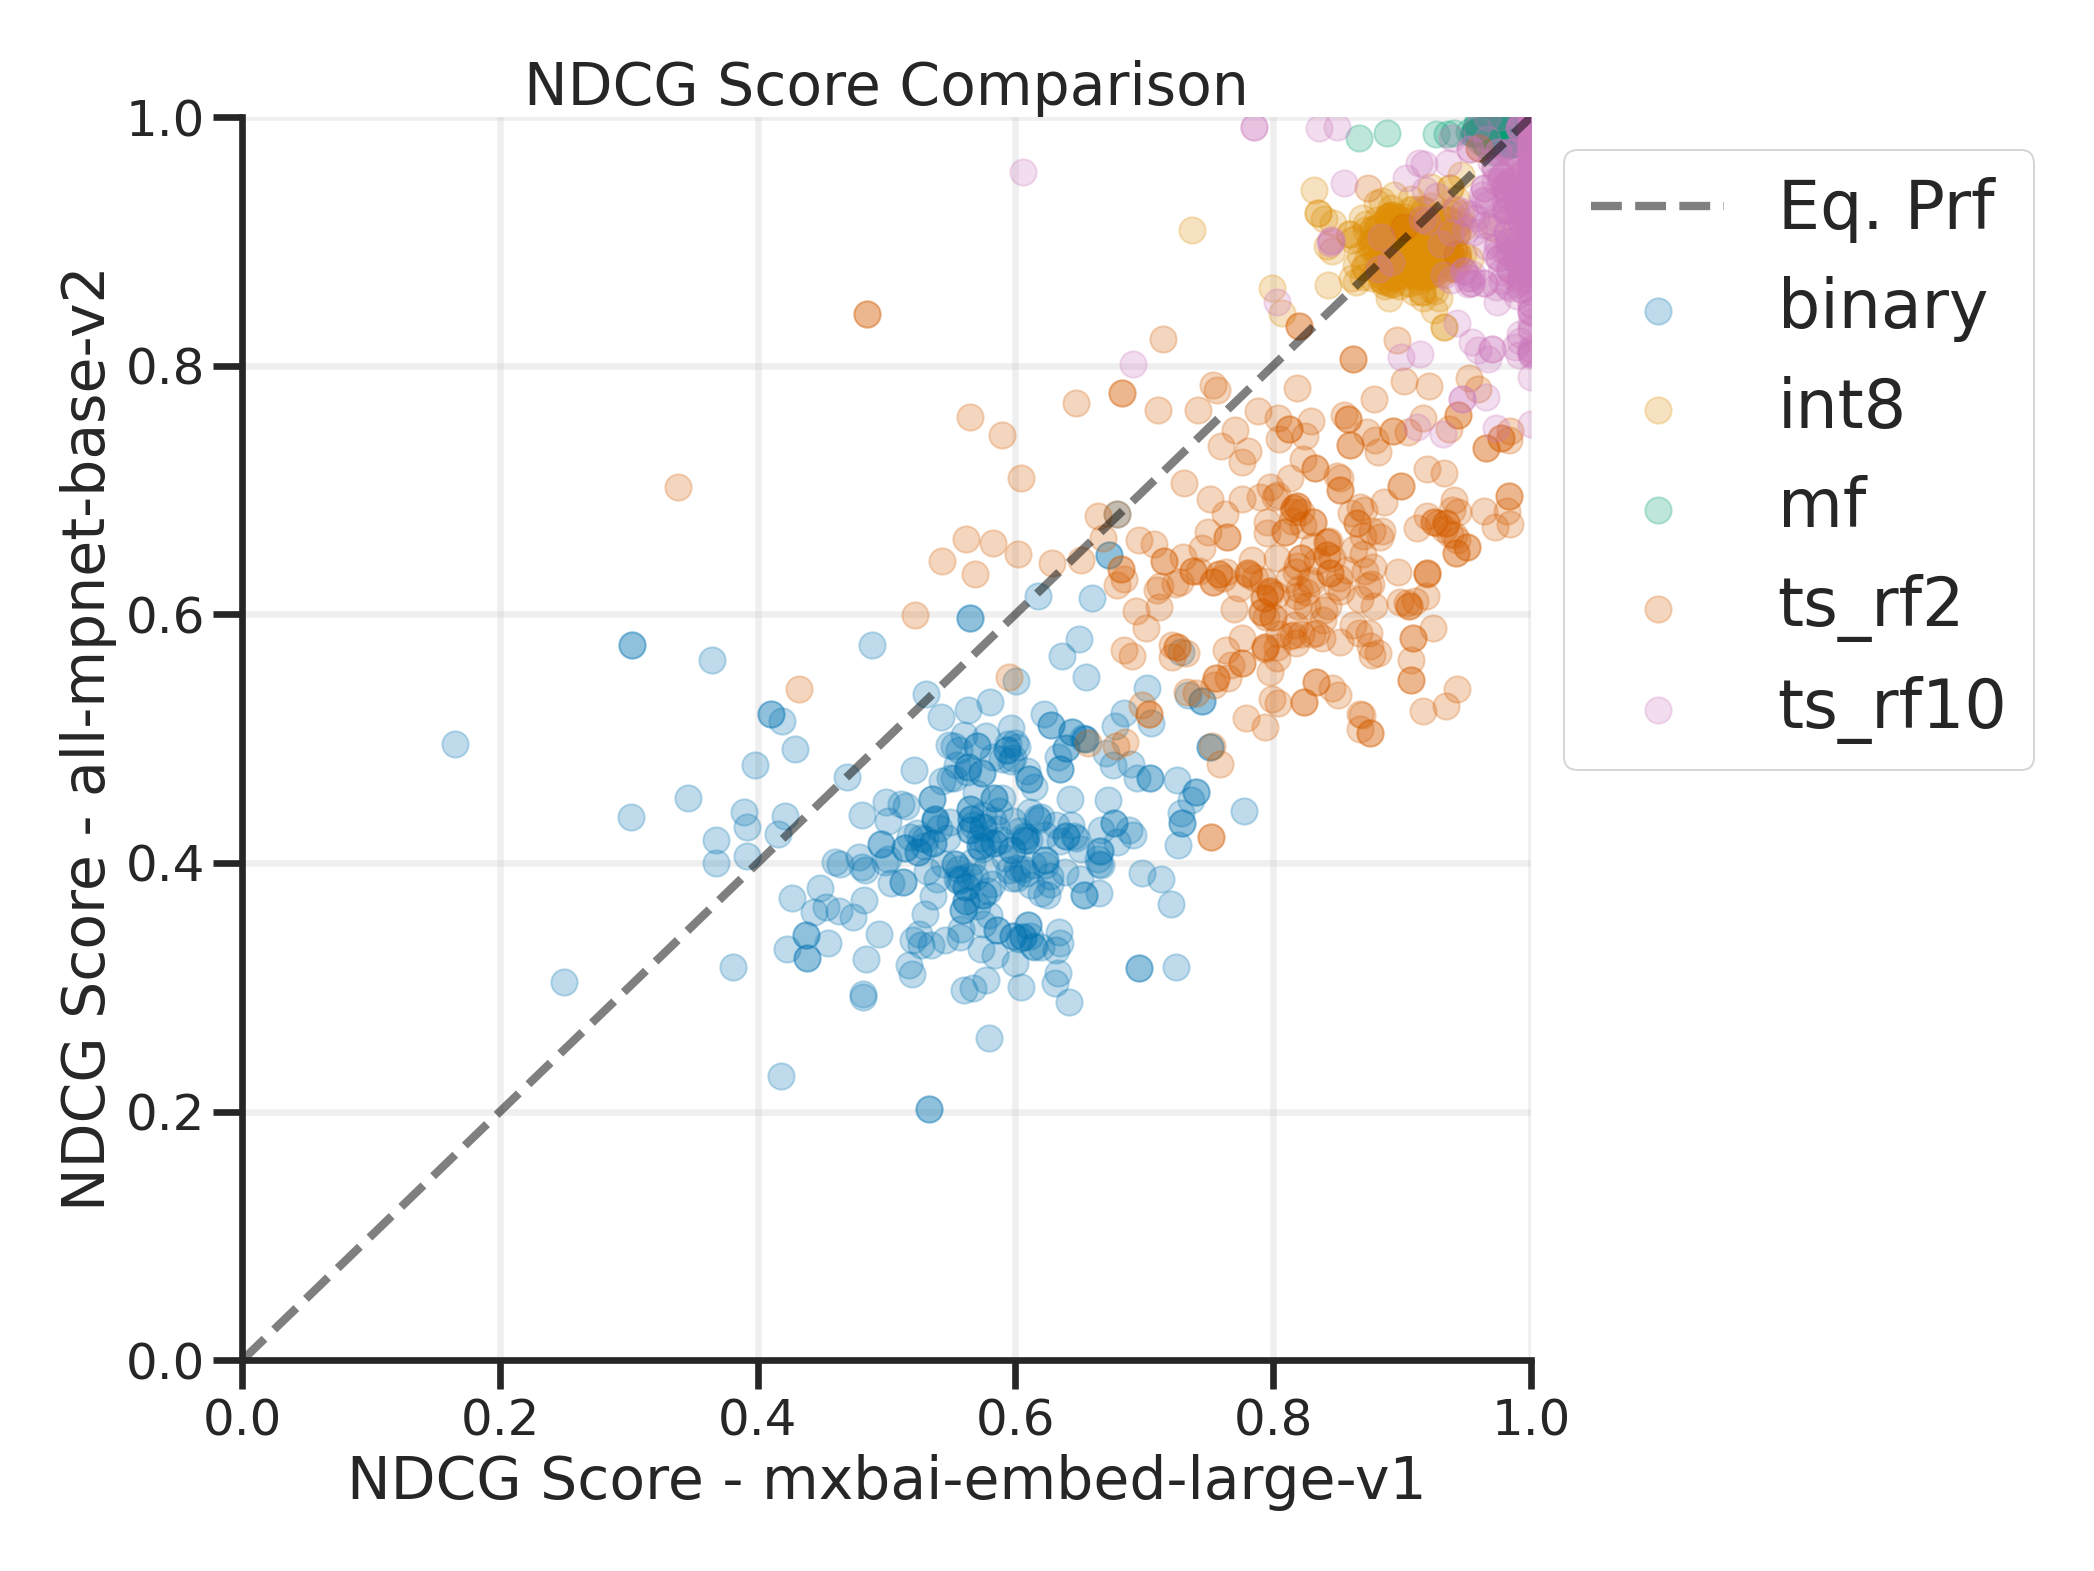
\includegraphics[width=0.49\widefigwidth]{bilder/plots/ndcg_scatter_benchmark_dim1024_k100_q_vs_benchmark_dim768_k100_q.png}
            \vspace*{-1cm}
            \caption{\scriptsize{NDCG score comparison between different models as scatter plot}}
            \label{ndcg_comp_diff_models_scatter}
        \end{minipage}
    }
\end{figure}
As mentioned earlier the model used is an angle optimized model, which should enable the binary searcher to get better results.~\cite{emb2024mxbai,li2024angleoptimizedtextembeddings}
To verify the previous results, the scores of the searchers when using the \texttt{\seqsplit{mixedbread-ai/mxbai-embed-large-v1}} model will be compared against the scores when using the \texttt{\seqsplit{sentence-transformers/all-mpnet-base-v2}} text embedding model. The same queries will be used.

Looking at the bar plot \autoref{ndcg_comp_diff_models} we see that the binary searcher indeed performs better with the angle optimized model. So does the two-step search as it's using the binary searcher in the first step. The PCA reduced searcher also perform better. This indicates, that the PCA algorithm is better at removing redundancies and grouping correlating dimensions for the embedding vectors created by the optimized model. There is no significant difference for the other searchers.

\subsection{Memory Usage Analysis}
\begin{figure}[h]
    \makebox[\textwidth][c]{%
        \begin{minipage}{0.49\widefigwidth}
            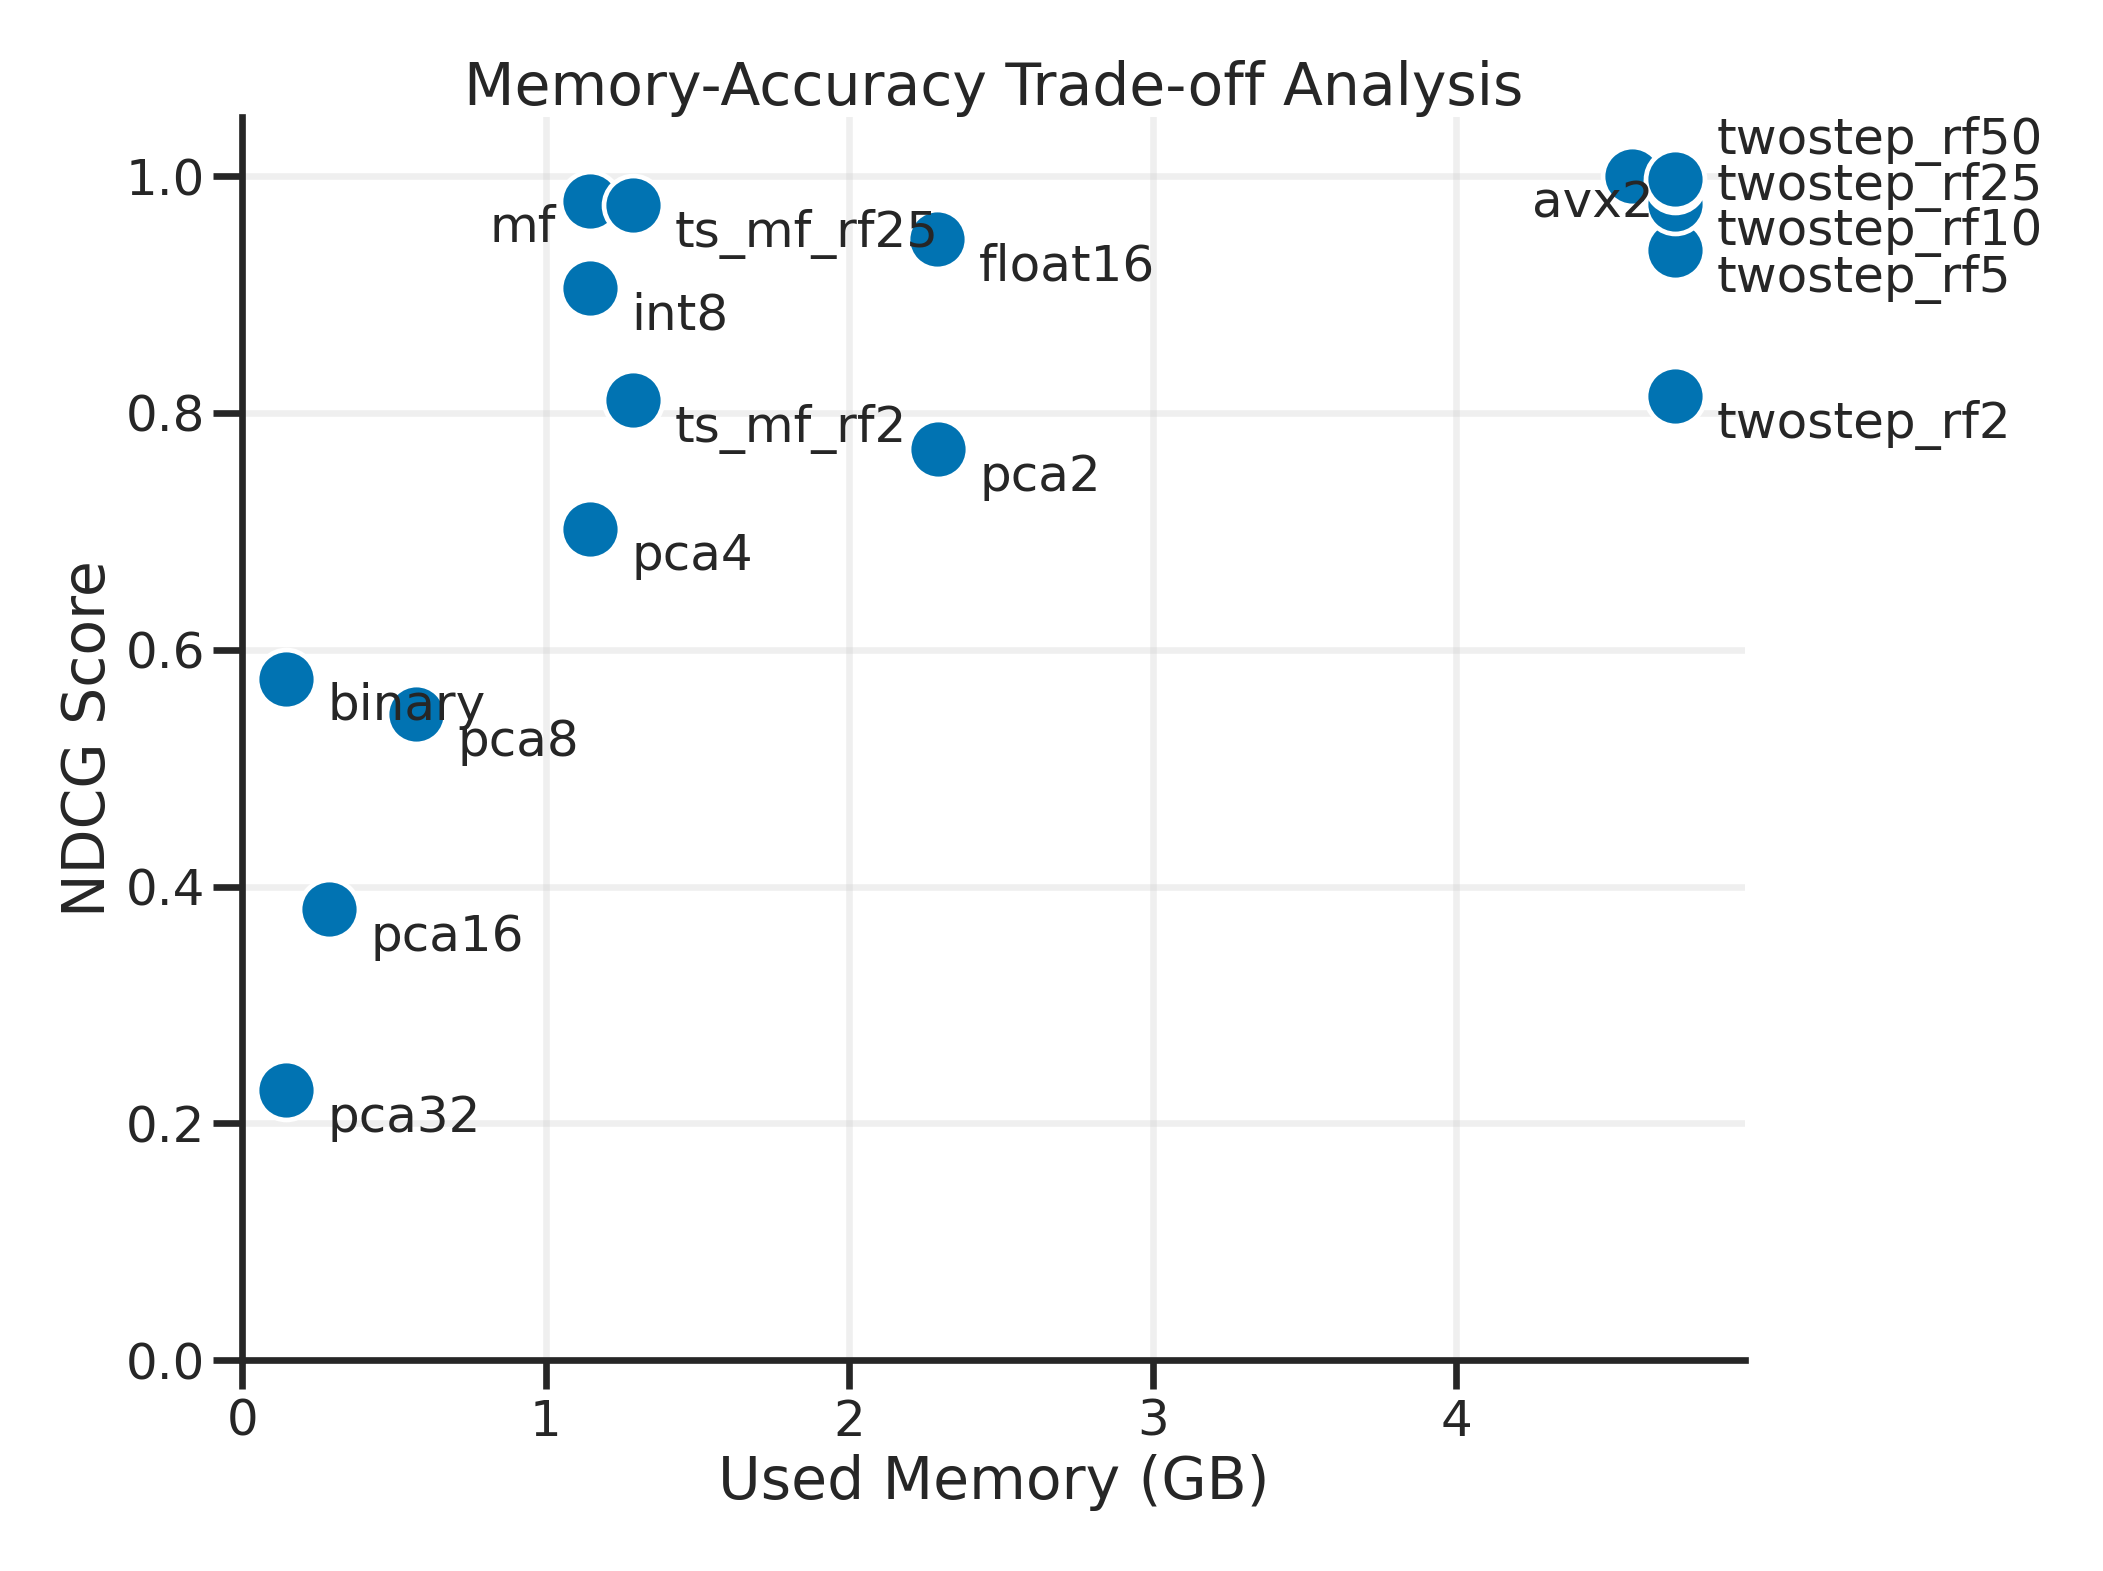
\includegraphics[width=0.49\widefigwidth]{bilder/plots/memory_vs_accuracy_dim1024_k100_q.png}
            \vspace*{-1cm}
            \caption{\scriptsize{NDCG Score vs Memory Usage}}
            \label{memory_vs_accuracy}
        \end{minipage}
        %\hfill
        \begin{minipage}{0.49\widefigwidth}
            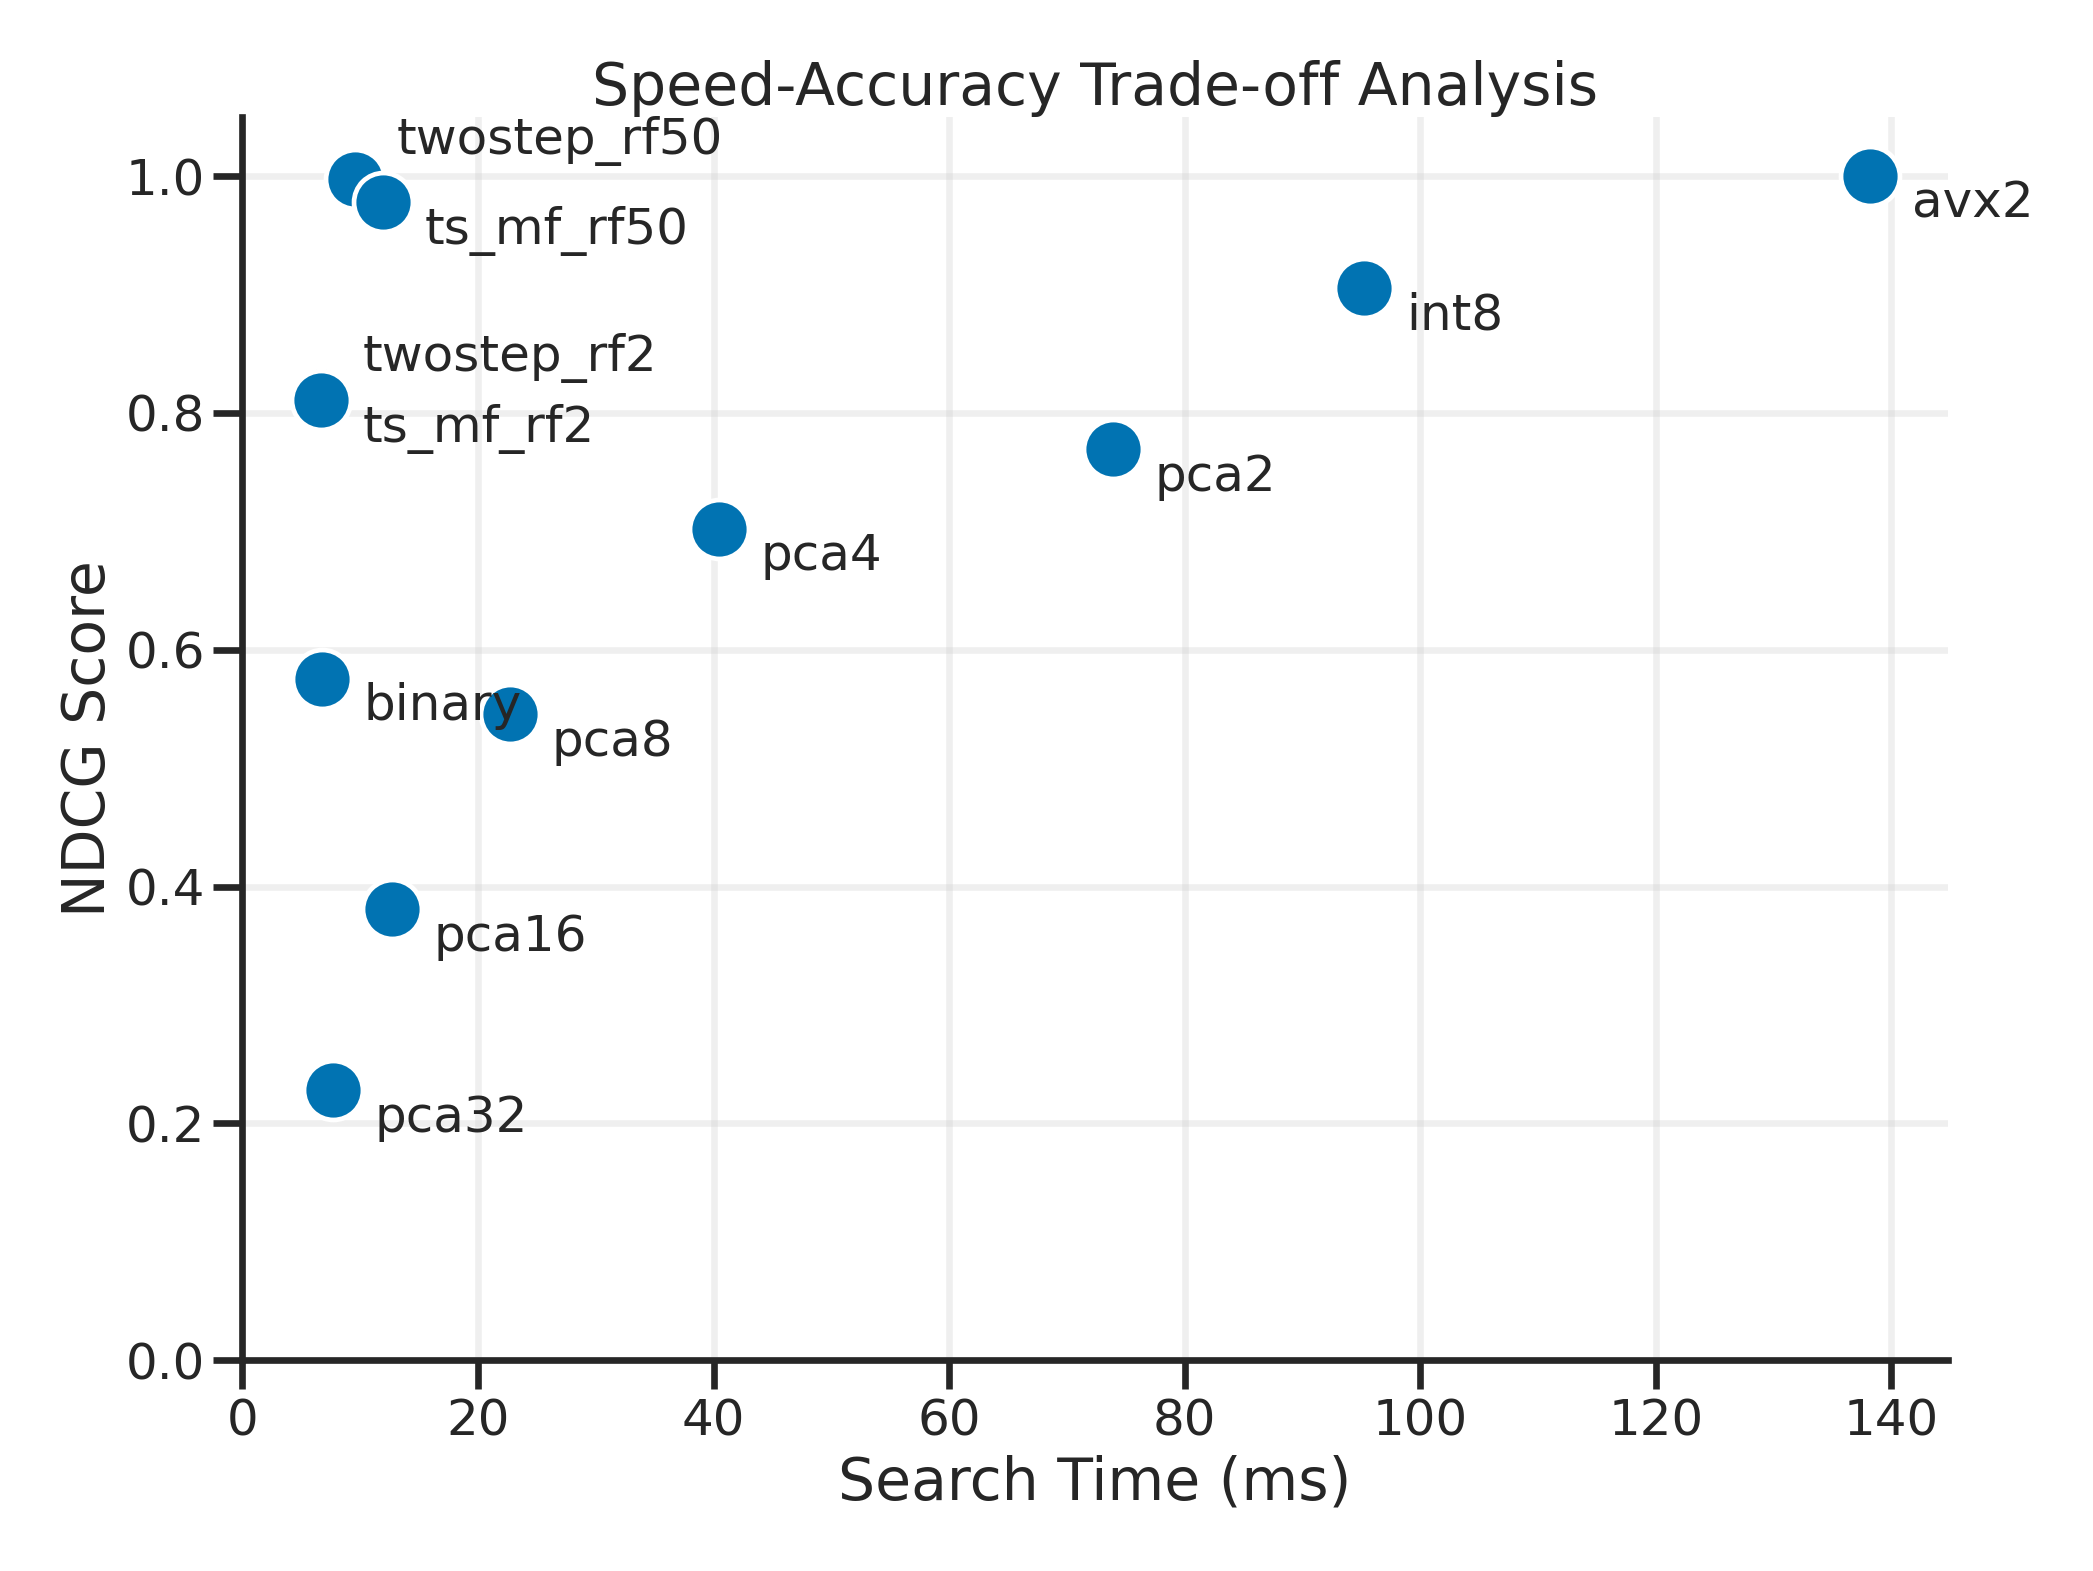
\includegraphics[width=0.49\widefigwidth]{bilder/plots/speed_vs_accuracy_dim1024_k100_q.png}
            \vspace*{-1cm}
            \caption{\scriptsize{NDCG Score vs Retrieval Time}}
            \label{memory_vs_speed}
        \end{minipage}
    }
\end{figure}
The binary+float searcher method uses the most memory, as it has to keep the binary and float32 embeddings in memory which totals to 33/32 times more memory usage compared to the baseline. Exactly the same memory usage as the baseline has the avx2 search, as it only optimizes the computation. And obviously the float16 variant uses half the memory of baseline.

The mapped float uses 1/4 of the baseline memory which makes it the best performing model in that memory range when factoring in its very high accuracy scores. This method is also one of the few not limited by memory bandwidth but by the L1 cache latency. Which makes it able to profit from multithreading on multicore CPUs as each core has its own L1 cache.

The binary+mapped float variant uses slightly more memory as it also has to load the binary embeddings, which, in return, makes it very fast. On its own the binary searcher uses the least memory except the PCA32 variant which has bad accuracy. The other PCA variants are also outperformed in search time and accuracy by other methods in the same memory range.

\subsection{Search Query Performance}
\begin{table}[h]
    \centering
    \begin{tabular}{l|ccccc|r}
        \toprule
        Query                                                           & \multicolumn{5}{c}{NDCG score} & type                                    \\
        \hline
                                                                        & binary                         & int8  & mf    & pca4  & ts\_rf10 &      \\
        \hline
        :)                                                              & 0.250                          & 0.799 & 0.867 & 0.202 & 0.691    & bad  \\
        paper                                                           & 0.302                          & 0.835 & 0.958 & 0.366 & 0.785    & bad  \\
        maps of places that don't exist yet                             & 0.392                          & 0.846 & 0.941 & 0.546 & 0.844    & bad  \\
        history of the number zero                                      & 0.464                          & 0.907 & 0.971 & 0.564 & 0.918    & bad  \\
        cars                                                            & 0.489                          & 0.881 & 0.957 & 0.623 & 0.966    & var  \\
        \footnotesize evolution of human color vision and its gene...   & 0.584                          & 0.921 & 0.984 & 0.691 & 1.000    & var  \\
        sun                                                             & 0.617                          & 0.892 & 0.982 & 0.575 & 1.000    & var  \\
        \footnotesize archaeological evidence of prehistoric human...   & 0.570                          & 0.878 & 0.990 & 0.720 & 1.000    & rand \\
        \scriptsize PLEASE HELP ME FIND INF[...] ABOUT DOLPHINS!!!      & 0.598                          & 0.914 & 0.978 & 0.791 & 0.976    & rand \\
        Roman legion size                                               & 0.604                          & 0.937 & 0.986 & 0.786 & 1.000    & good \\
        \footnotesize development of early mechanical calculators in... & 0.575                          & 0.938 & 0.990 & 0.770 & 1.000    & good \\
        pizza pizza pizza pizza pizza pizza pizza                       & 0.778                          & 0.971 & 0.995 & 0.839 & 1.000    & good \\
        \bottomrule
    \end{tabular}
    \caption{Accuracy for different search queries}
    \label{queryanalysis}
\end{table}

In the \autoref{queryanalysis} are some queries listed that were also used in the benchmarks. The table lists the corresponding scores for some search implementations. 4 categories of queries were selected: Good and bad performing queries, queries with high score variance and randomly selected queries. The worst performing query is just a ":)" it's an unconventional query that has no point. Even a human would have problems interpreting a distinct semantic meaning into it. But still, the int8, mapped float and two-step method perform quiet well. The binary and PCA4 score is with around 0.2 really low. But this explains the big outliers in the box plots \ref{boxjaccardsearchersone} \ref{boxndcgsearchersone} \ref{boxjaccardsearcherstwo} \ref{boxndcgsearcherstwo}. Which makes the outliers less bad, because you can't expect good results from a query like this. "paper", a really generic query that also has quiet low scores, especially for the binary and PCA4 searcher. The other implementations perform good enough with this query. An example for more specific queries would be "Roman legion size". Here its very apparent what the user would want as an answer. All searchers have good score with this query.

In conclusion, more specific queries, which also implies more semantic meaning, seem to perform better. It also explains the outliers of the lower accuracy models and gives more confidence in rating them as usable.



\section{Summary}
Most results are roughly in line with the expectations. The accuracy of the mapped float searcher is very surprising. The fact it performs better than float16 with only 8 bits was unexpected. But the reason for this could be the accuracy loss during float addition. During the calculation of the dot product the products of the vector dimensions are added to the dot product where each addition can generate accuracy loss. And for the float16 this running sum is also in float16 format, while the mapped float uses float32 for this, as its using float32 values during multiplication.

The slow speed of the int8 search can be explained by the instruction intensive splitting, moving and extending of vectors/values, which is needed to prevent overflow. Maybe quantization with a limit of 4 used bits would be better, as one could then simply multiply the int8 values without risking overflow.

PCA performed much worse than expected as even PCA2s accuracy is outperformed by simple int8 quantization.

Also, the binary and two-step methods are overall the most useful as they are very fast. For the two-step methods comes the addition of being very accurate. And two-step with the mapped float even hast a fairly low memory usage which makes it overall the best performers when considering all 3 main metrics of memory usage, accuracy and speed.
\chapter{Future Work}
\label{chapter:future_work}
This chapter gives ideas on future research directions for vector similarity search optimization, based on the findings presented in this thesis.

\section{Disk-Based Two-Step Search}
The presented two-step implementations keep all embeddings of both searchers in memory, which limits its usage on devices with constrained memory. A promising extension would be disk based approach that work like this: The binary embeddings are stored in memory. This reduces the memory usage by 1/32 compared to full precision.
The embeddings of the second searcher (full accuracy or mapped float for example) for rescoring stay on disk in a format that allows fast retrieval of embeddings. Then the binary search is used to get promising candidates. In the second step the high precision embeddings from these candidates are loaded from disk. For 10 documents with a rescoring factor of 25 and a disk access time of 1ms this would take $10*25*1ms=250ms$. But this can potentially be way faster with an optimized I/O strategy. And most modern flash storage has a latency of less than 1ms. Another challenge is designing an efficient disk storage format that allows fast random access to the specific embeddings. Additionally, frequently accessed embeddings could be cached.

\section{Hardware Specific Optimizations}
\subsection{Float16 Hardware support}
In the future more processors should have native support for float16 operations. AVX512 can, for example, load 32 float16 values into one 512 bit register. Float16 had very good accuracy and should be much faster than float32 on supported hardware. Hardware accelerated float16 should be used when available. Many modern GPUs also support float16 and advertise double throughput compared to full precision.

\subsection{ARM NEON support}
This thesis focused on AVX2 optimizations. But many mobile and embedded devices use ARM processors. Future work could port the SIMD optimizations to NEON instructions, as most AVX2 instructions have a NEON equivalent counterpart. This would also allow to compare the optimizations between ARM and x86.

\section{Additional Optimization Approaches}
Some promising optimizations warrant more investigation:
\subsection{Hybrid/Adaptive Quantization Methods}
\begin{itemize}
    \item Quantization that quantizes with different precision levels for different parts of the vector.
    \item Compress parts of the vector that has repeating or similar information. This probably becomes especially effective when have already low precision elements. At 8 bit for example, there are way more elements in a vector than distinct values they can have (256 values and 1024 elements).
\end{itemize}

Another better approach to reduce the embedding size than PCA dimension reduction is the usage Learning-to-Hash algorithms as they outperform PCA for embeddings.~\cite{thakur2023injectingdomainadaptationlearningtohash}

\subsection{Memory Access Optimization}
Different layouts of the embedding matrix to optimize bandwidth could be investigated. Also, the reasons for strided access being faster are not clear and should be looked into.

\section{Research directions}
\subsection{Domain Specific Optimization}
As this thesis only worked with text embeddings, future research could explore how different domains (text, image, audio, ...) affect optimization effectiveness. Especially with techniques like the mapped float embeddings.
Additionally, the impact of different embedding models could be analyzed. With the results from this one could investigate domain specific optimizations.

\subsection{Theoretical Analysis}
The relationship between binary quantization or PCA with angular similarity needs further investigation. As both have a big accuracy difference between traditional embedding models and the angle optimized model.

\section{Real World Applications}
Future work could also focus on these real world applications:
\begin{itemize}
    \item Implementation in production search systems.
    \item Implementation in existing vector databases.
    \item Creating more standardized benchmarks for vector search.
    \item Analyze optimization strategies for different use cases.
\end{itemize}

\noindent All these directions would build on the foundation created by this thesis and would advance the efficient vector similarity search on resource constrained devices.
\chapter{Conclusion}
\label{chapter:conclusion}
This thesis investigated various optimization techniques for vector similarity search with focus on increasing performance, keeping good accuracy and lowering the memory required to enable better search on resource constrained devices. With extensive experimentation followed by good analysis of the recorded results, it has made multiple contributions towards further optimizations for vector similarity search.

\section{Summary of findings}
The baseline float32 implementation was the metric against which the optimizations were compared. The findings from experimenting and analyzing different optimizations are as follows:

\subsection{Quantization Methods}
Overall the quantization based methods performed very good. Int8 quantization achieved a 4x reduction in memory usage while main around 90\% accuracy.
The binary quantization performed even better: With 32x memory reduction while maintaining $\sim$58\% accuracy. This performance dropped to slightly over 40\% with a non-angle optimized model.
It is about 20 times faster than the highly optimized float32 implementation with AVX2 and around 160 times faster than the naive float32 implementation. The biggest improvement came from switching the native 64bit popcount with a lookup table based popcount using AVX2. Another interesting result is from the mapped float approach, which combines quantization, adapting to dataset and value mapping. It achieved 97\% accuracy while quartering the memory usage. It was the highest accuracy non-float32 searcher, even outperforming float16.
But looking at \autoref{mfvaluedist} its likely that the Gauss distribution actually just matches the distribution of values contained in the embeddings very closely. That might also be the reason why the Quantization mapping in \autoref{mfquantmapping} might be so linear. But to confirm this suspicion one should compare int8 Quantization where then int8 minimum value maps to the minimum values contained in the embeddings and int8 maximum value maps to the max value contained in the  embeddings. The values in between should just be scaled linearly.

\subsection{SIMD Optimization}
The AVX2-optimized float32 implementation achieved 8x speedup over the baseline. At the end the memory bandwidth became the bottleneck. The method of comparing the query vector to multiple embeddings at once was highly effective as it greatly reduces the number of loads from memory/cache. This also increased the memory bandwidth.
The int8 implementation gained less performance from the AVX2 implementation as it has to move the data around quiet a bit before being able to multiply the values. Additionally, it can only multiply 16 int8 values at a time. But there are other instructions, I didn't discover in time, like \textit{PMADDUBSW} which multiples 32 int8 and adds the int16 results of neighboring numbers together.

\subsection{Two-Step Approach}
Binary pre-filtering followed by high precision rescoring is highly effective. With a rescoring factor of 10 it achieved a NDCG score of 97.7\% with float32 rescoring and 96.3\% with mapped float rescoring. Both just very slightly increased the search time.
This demonstrated, that this approach is highly effective. It's very close to binary speed and very close to float32 accuracy. With the mapped float as second step it additionally only uses 9/32 of the baseline memory.

\subsection{Dimension Reduction}
The dimension reduction using the PCA technique had worse accuracy than quantization methods with comparable memory savings. This makes it not useful for accelerating search and saving memory. This is also mentioned in this paper:~\cite{thakur2023injectingdomainadaptationlearningtohash} Other dimension reduction- or vector compression methods should be investigated.

\section{Key Insights}
\subsection{Memory Access Patterns}
Memory access pattern showed to be very important as most implementations were bottle necked either by memory bandwidth or latency. Optimizing towards memory bandwidth/latency is very important as the actual calculations are very fast.
Strided access increased bandwidth even though its common knowledge that strided access is usually slower than purely sequential access. The systems' memory pages, memory ranks or memory interleaving are a suspected reason for this behavior.
Prefetching, either manually or automatically by the CPU, is also very important and effective as it's able to hide the extremely high system memory latency.

\subsection{Quantization Trade-Offs}
The different quantization methods showed distinct trade-offs between accuracy and performance. Furthermore, the embedding model can influence the performance of the quantization methods. The mapped float approach demonstrated, that "intelligent" quantization can preserve more semantic meaning than linear quantization with the same memory usage.

\subsection{Hardware Utilization}
SIMD instructions can provide a substantial performance improvement. With this memory bandwidth becomes a limiting factor fast. Even though the implementations don't use multithreading at all.

\section{Limitations and Future Work}
All methods implemented keep the embeddings in memory at all times. Which may not be needed especially for the two-step approach. Then it only has to load the embeddings from the documents needed for rescoring form disk. Additionally, the SIMD optimizations are specific to the x86 architecture but should be able to be transferred to other architectures using similar instructions. The findings should also be verified on different architectures.

\section{Final Remarks}
It was demonstrated, that significant performance improvements in vector similarity search can be achieved by optimizing hardware usage and using quantization. Especially combining smart quantization, SIMD and the two-step approach provide close to full accuracy, while being 100 times faster than baseline and more than 10 times faster than the optimized full accuracy search. All while using less memory. Which can be very beneficial for resource constrained devices.
% % Anhang
\appendix
% anhang.tex
\chapter{Appendix}
\label{chapter:appendix}
\section{Isolated Testing of Memory Bandwidth}
\label{section:stridedmembwtest}
\begin{figure}[h]
  \begin{algorithm}{Loop with Strided Memory Access}{stridedmemoryaccess}
    \begin{lstlisting}[language=C++,basicstyle=\scriptsize\ttfamily,showstringspaces=false]
// Uses 8 strides spaced out 4 KB
for (int iter = 0; iter < NUM_ITERATIONS; iter++) {
  for (size_t i = 0; i < VEC_SIZE - TOTAL_STRIDE_DIST + 1;
       i += TOTAL_STRIDE_DIST) {
    #pragma GCC unroll 1 // prevent loop unrolling
    for (size_t j = i; j < STRIDE_LENGTH + i; j += 8) {
      asm volatile(                        //
          "vmovaps (%0),       %%ymm0\n\t" //
          "vmovaps 0x1000(%0), %%ymm1\n\t" // offset 1 * 4096 bytes
          "vmovaps 0x2000(%0), %%ymm2\n\t" // offset 2 * 4096 bytes
          "vmovaps 0x3000(%0), %%ymm3\n\t" // offset 3 * 4096 bytes
          "vmovaps 0x4000(%0), %%ymm4\n\t" // offset 4 * 4096 bytes
          "vmovaps 0x5000(%0), %%ymm5\n\t" // offset 5 * 4096 bytes
          "vmovaps 0x6000(%0), %%ymm6\n\t" // offset 6 * 4096 bytes
          "vmovaps 0x7000(%0), %%ymm7"     // offset 7 * 4096 bytes
          :
          : "r"(&array[j])                  //
          : "ymm0", "ymm1", "ymm2", "ymm3", //
            "ymm4", "ymm5", "ymm6", "ymm7");
    }
  }
} // Uses sequential memory access
for (int iter = 0; iter < NUM_ITERATIONS; iter++) {
  #pragma GCC unroll 1 // prevent loop unrolling
  for (size_t i = 0; i < VEC_SIZE - 63; i += 64) {
    asm volatile(                      //
        "vmovaps (%0),     %%ymm0\n\t" //
        "vmovaps 0x20(%0), %%ymm1\n\t" // offset 32 bytes <=> 1 AVX2 vector
        "vmovaps 0x40(%0), %%ymm2\n\t" // offset 64 bytes
        "vmovaps 0x60(%0), %%ymm3\n\t" // ...
        "vmovaps 0x80(%0), %%ymm4\n\t"
        "vmovaps 0xa0(%0), %%ymm5\n\t"
        "vmovaps 0xc0(%0), %%ymm6\n\t"
        "vmovaps 0xe0(%0), %%ymm7"
        :
        : "r"(&array[i])                  //
        : "ymm0", "ymm1", "ymm2", "ymm3", //
          "ymm4", "ymm5", "ymm6", "ymm7");
  }
}
    \end{lstlisting}
  \end{algorithm}
\end{figure}
\noindent A C program to test the bandwidth of strided against non-strided memory access was created to isolate "the problem" from other variables. In \autoref{alg:stridedmemoryaccess} are the two loops used in the methods testing the memory read bandwidth. The loops iterate 16 times over a 12 GB array. These are the results from two different machines:
\\\texttt{
  Results from Machine used in previous experiments:\\
  SIMD Read Bandwidth (Sequential)\ \ \ \ \ \ \ \ \ \ \ : 29.46 GB/s\\
  SIMD Read Bandwidth with stride length 4096: 36.71 GB/s\\
  AMD 4800U 8C/16T, 16 GB LPDDR4 2666MHz:\\
  SIMD Read Bandwidth (Sequential)\ \ \ \ \ \ \ \ \ \ \ : 16.39 GB/s\\
  SIMD Read Bandwidth with stride length 4096: 22.74 GB/s\\
}
The results line up very closely with the bandwidth results obtained from the vector similarity search program. But I have no Intel PC at my disposal to test this on a different architecture.

\section{Trying out the Similarity Search Implementation}
\label{sec:tryingout}
Go to \url{https://github.com/thubn/simsearch} for more information. In the main README go to the "Embedding Search Server" link in the index.

\section{Additional Plots}
\begin{figure}[h]
  \makebox[\textwidth][c]{%
    \begin{minipage}{0.49\widefigwidth}
      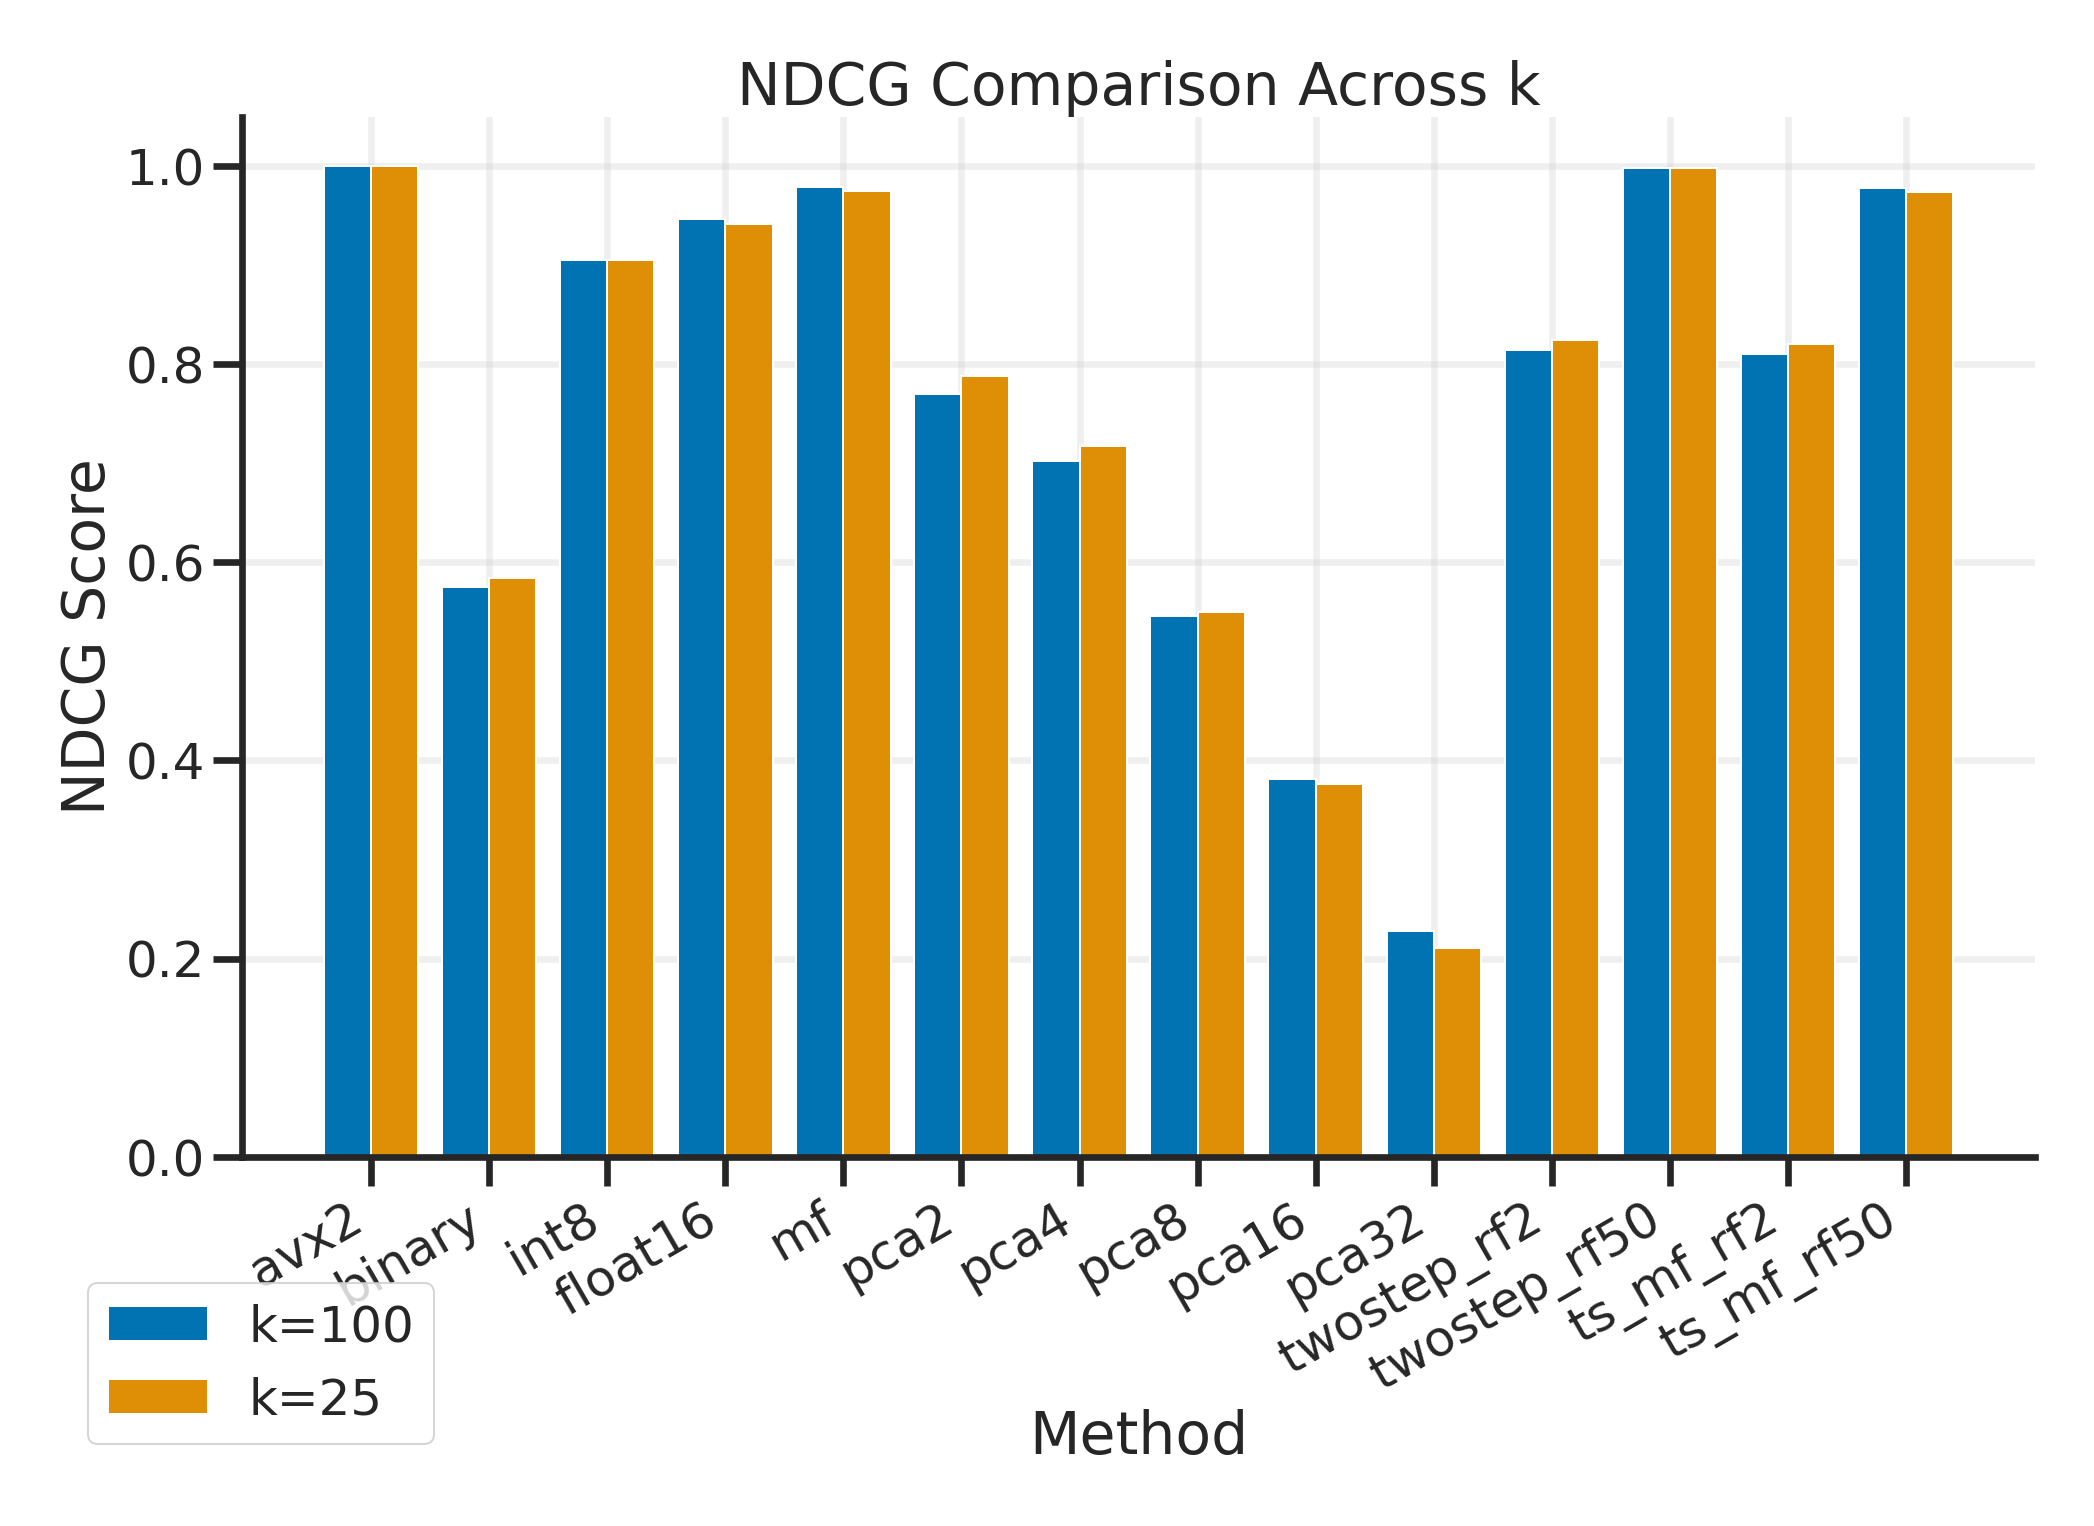
\includegraphics[width=0.49\widefigwidth]{bilder/plots/benchmark_comparison_dim1024_k100_q_dim1024_k25_q_cmp_k.png}
      \vspace{-1cm}
      \caption{Comparing the retrieval accuracy across different k values}
      \label{kcomparison}
    \end{minipage}
    %\hfill
    \begin{minipage}{0.49\widefigwidth}
      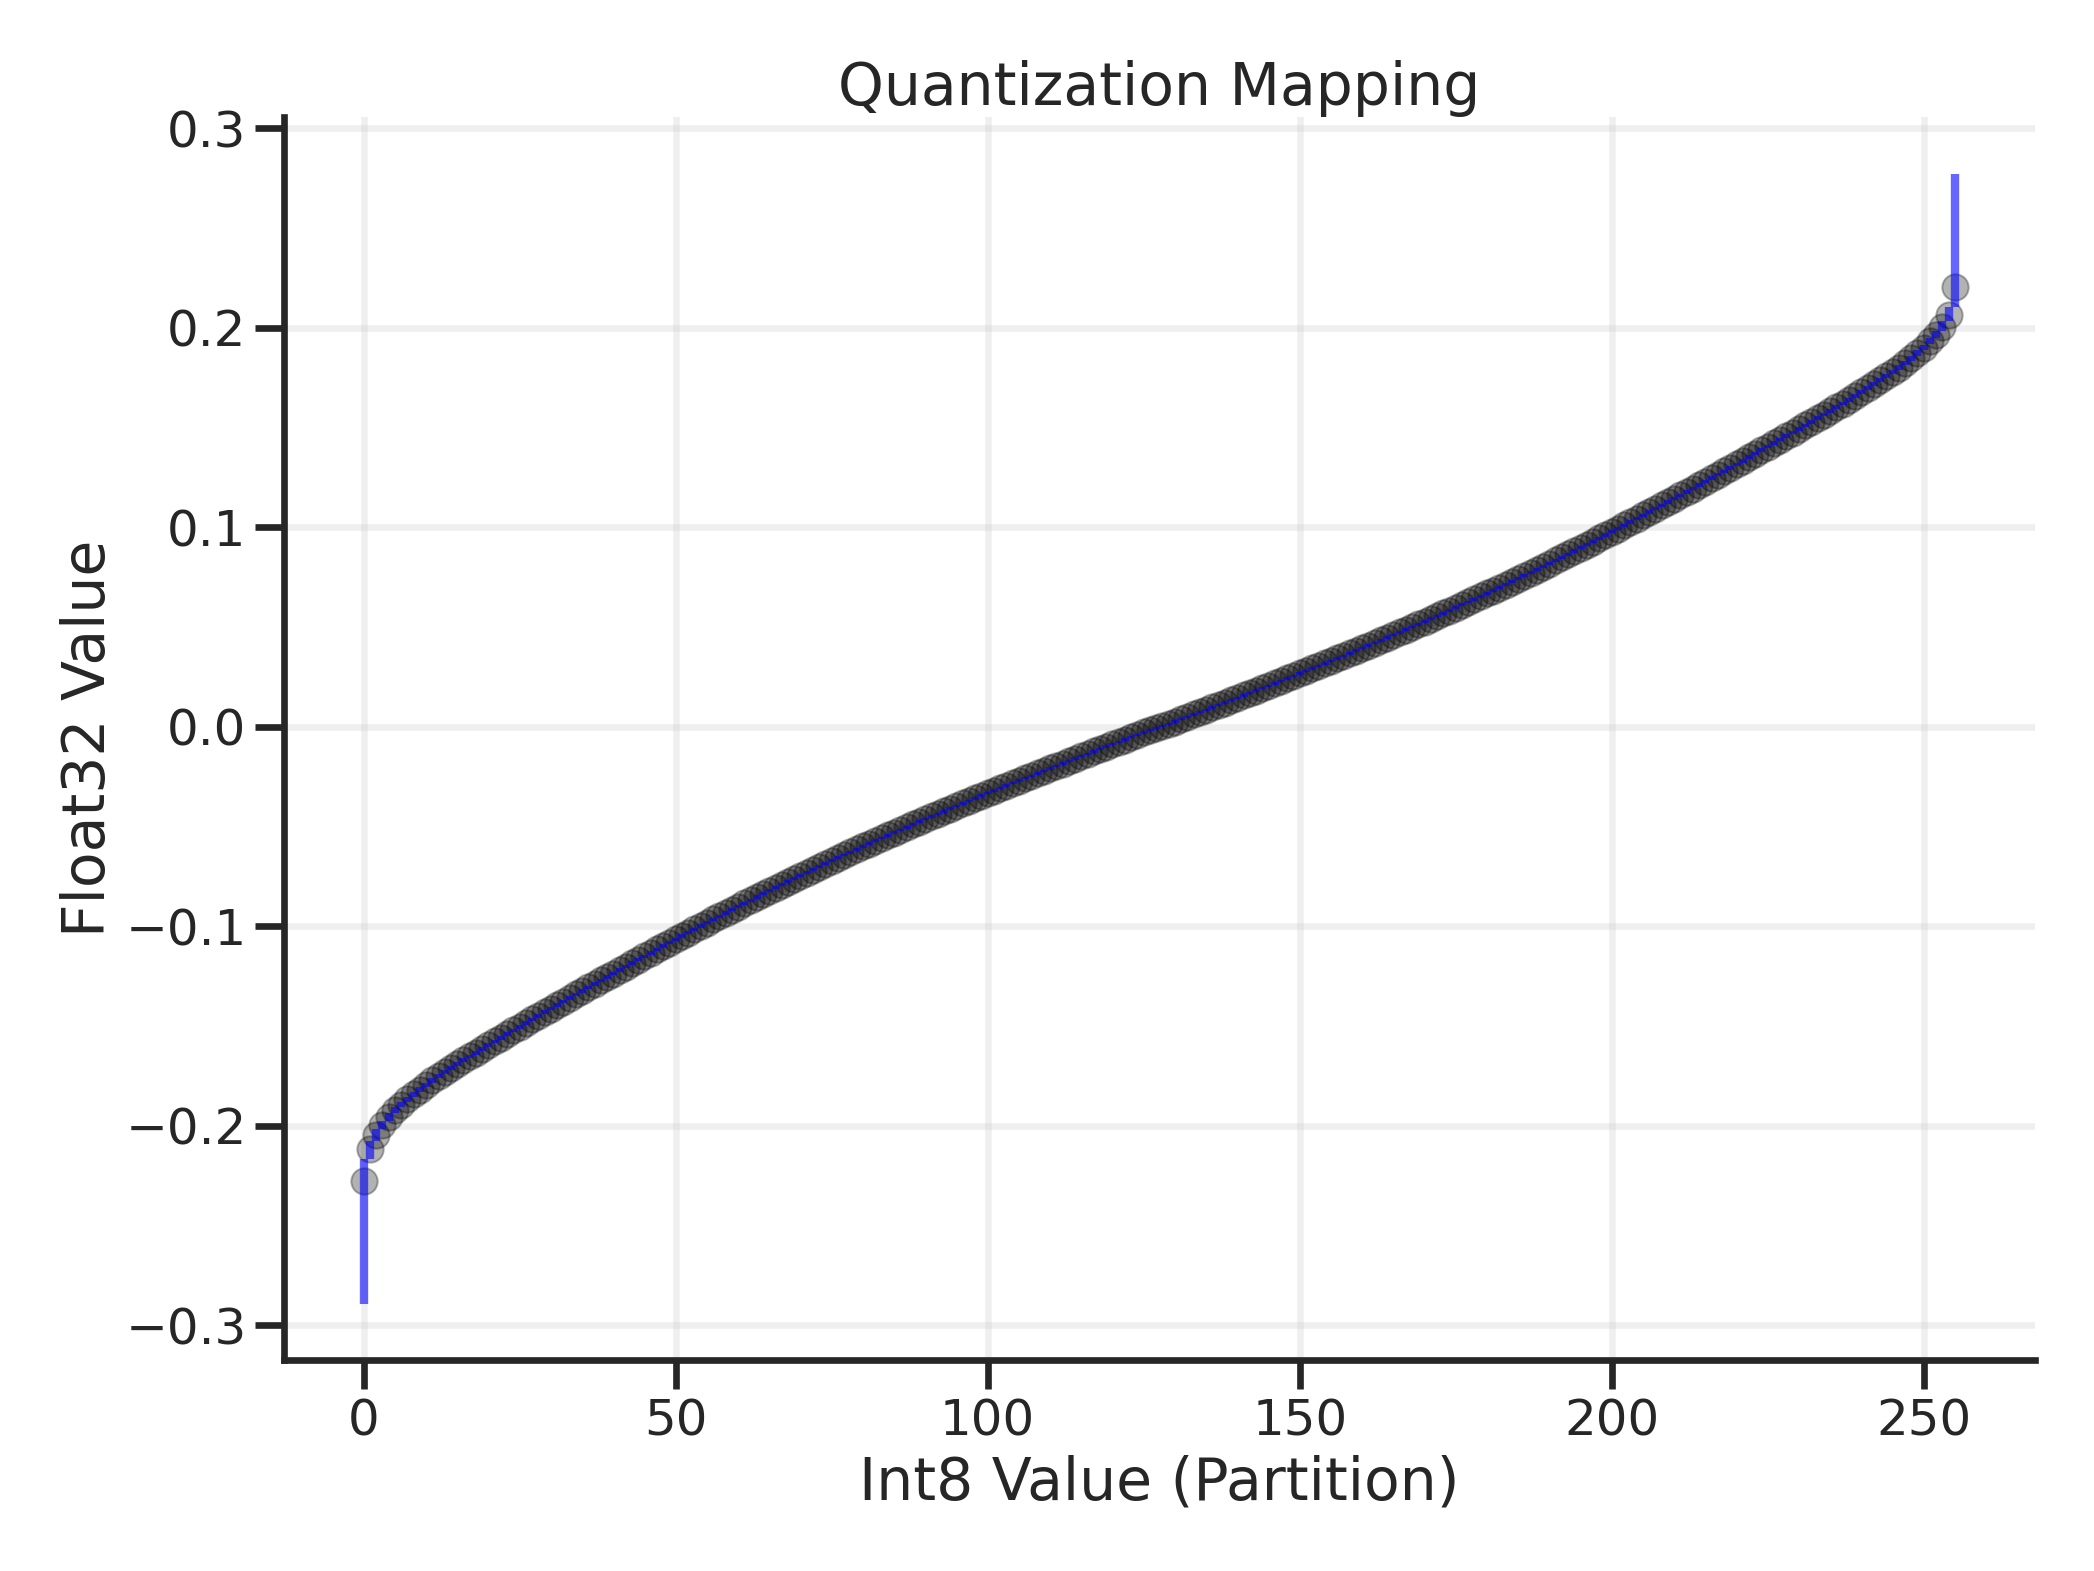
\includegraphics[width=0.49\widefigwidth]{bilder/plots/quantization_mapping_768.png}
      \vspace{-1cm}
      \caption{Mapped Float Quantization mapping for the sentence-transformers/all-mpnet-base-v2 model}
      \label{quantmapping768}
    \end{minipage}
  }
\end{figure}
\noindent The quantization mapping seen in \autoref{quantmapping768} of the embeddings from model \texttt{\seqsplit{sentence-transformers/all-mpnet-base-v2}} doesnt have a gap like the angle optimized model.\\\\
Varying k as seen in \autoref{kcomparison} doesn't create a big difference in accuracy.

\begin{figure}[h]
  \makebox[\textwidth][c]{%
    \begin{minipage}{0.49\widefigwidth}
      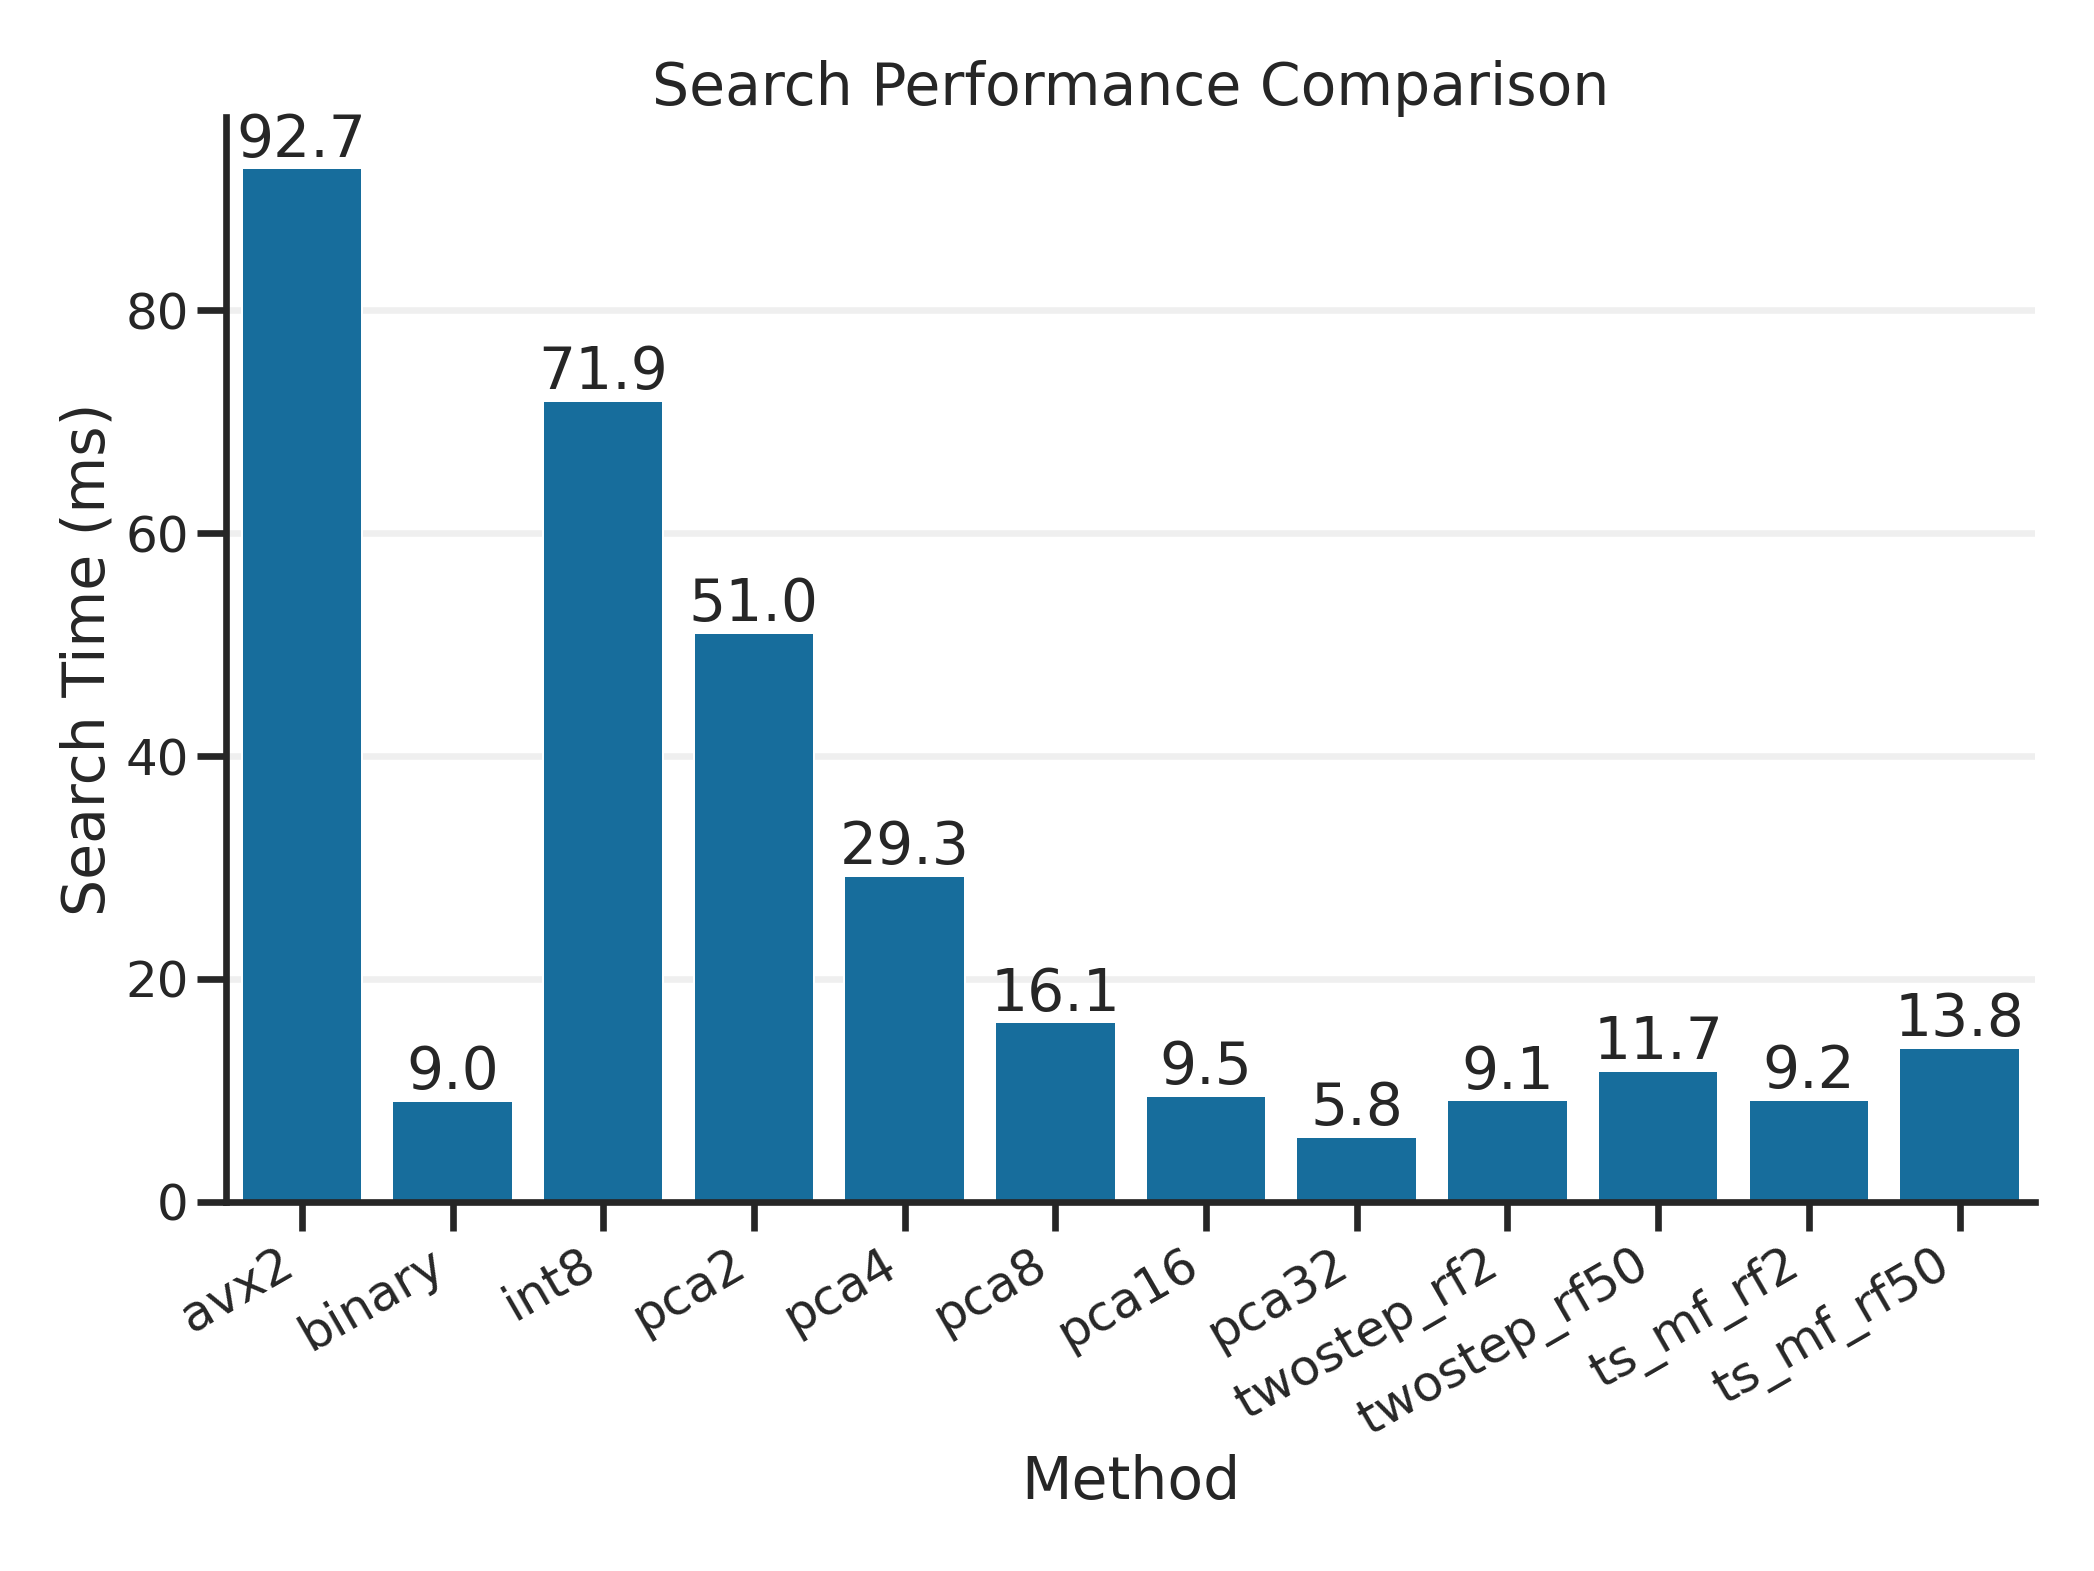
\includegraphics[width=0.49\widefigwidth]{bilder/plots/performance_comparison_dim768_k100_q.png}
      \vspace{-1cm}
      \caption{Search Speed vec\_dim=768 model: sentence-transformers/all-mpnet-base-v2}
    \end{minipage}
    %\hfill
    \begin{minipage}{0.49\widefigwidth}
      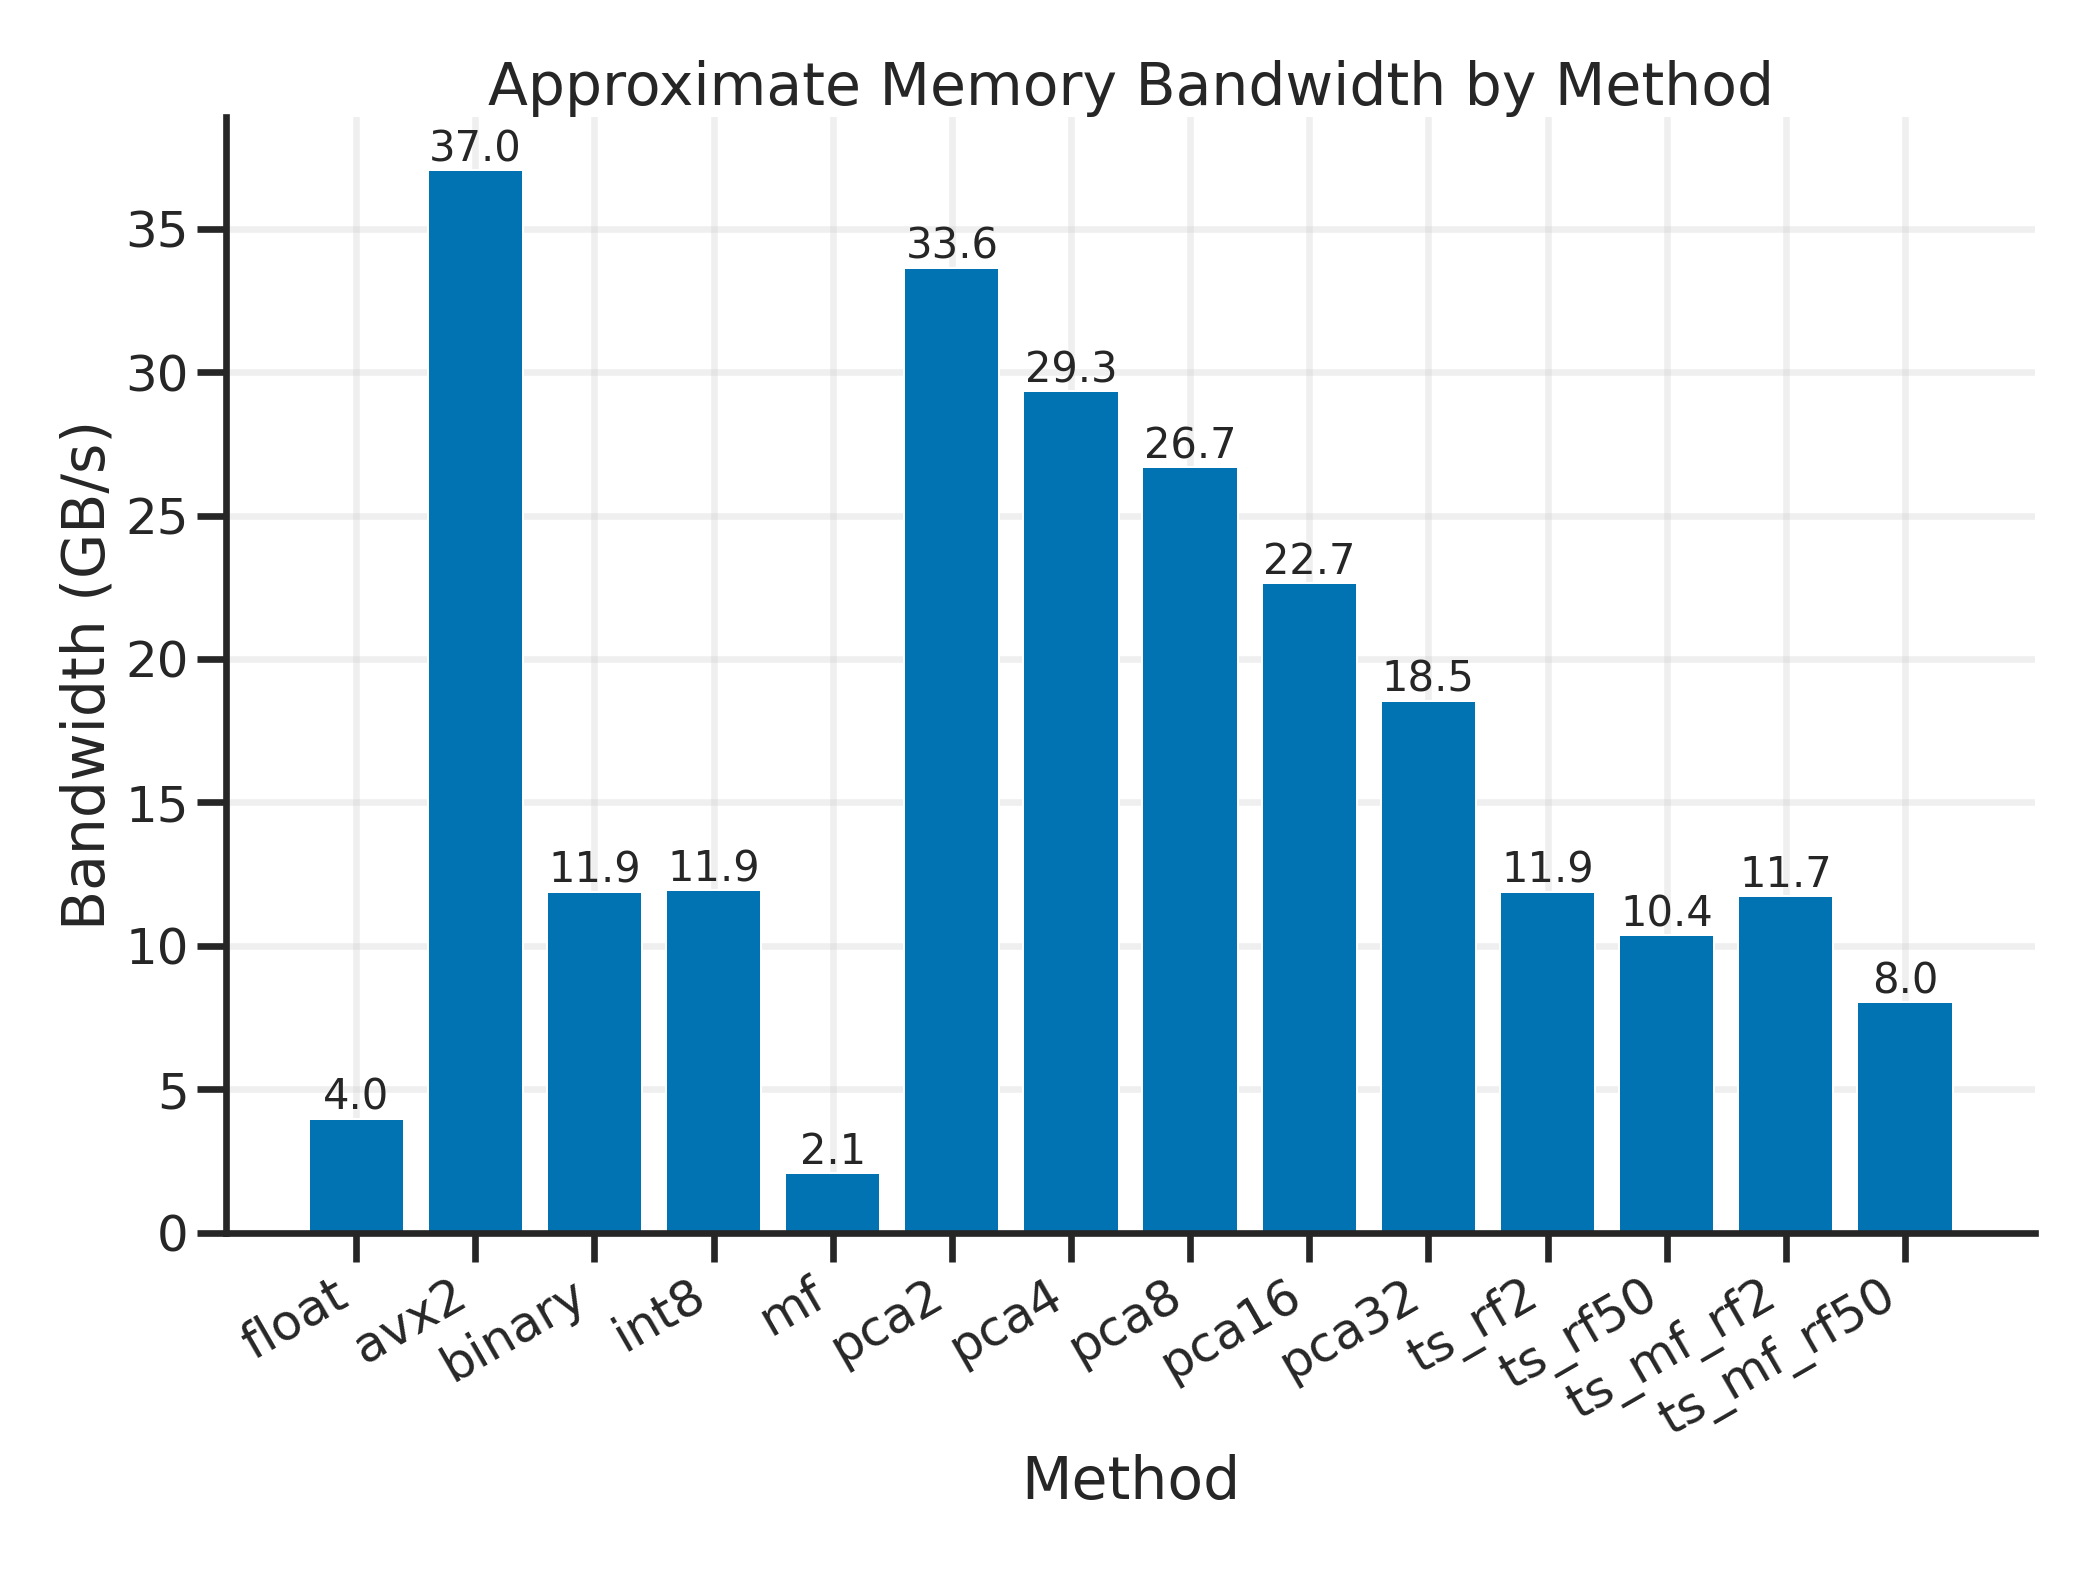
\includegraphics[width=0.49\widefigwidth]{bilder/plots/memory_bandwidth_benchmark_dim768_k100_q.png}
      \vspace{-1cm}
      \caption{Memory bandwidth vec\_dim=768 model: sentence-transformers/all-mpnet-base-v2}
      \label{memorybandwidth768}
    \end{minipage}
  }
\end{figure}
\noindent The memory bandwidth in \autoref{memorybandwidth768} when using the \texttt{\seqsplit{sentence-transformers/all-mpnet-base-v2}} model is even higher. The reason might be that higher striding distance is even better as this model creates embeddings of size 3072 bytes, so it has to use a striding distance of 12288 bytes as it's the first multiple that's divisible by 4096. Binary performs worse because it can't use the optimized unrolled loop as it only uses 3 avx2 vectors for 768 dimensions.

\begin{figure}[h]
  \makebox[\textwidth][c]{%
    \begin{minipage}{0.49\widefigwidth}
      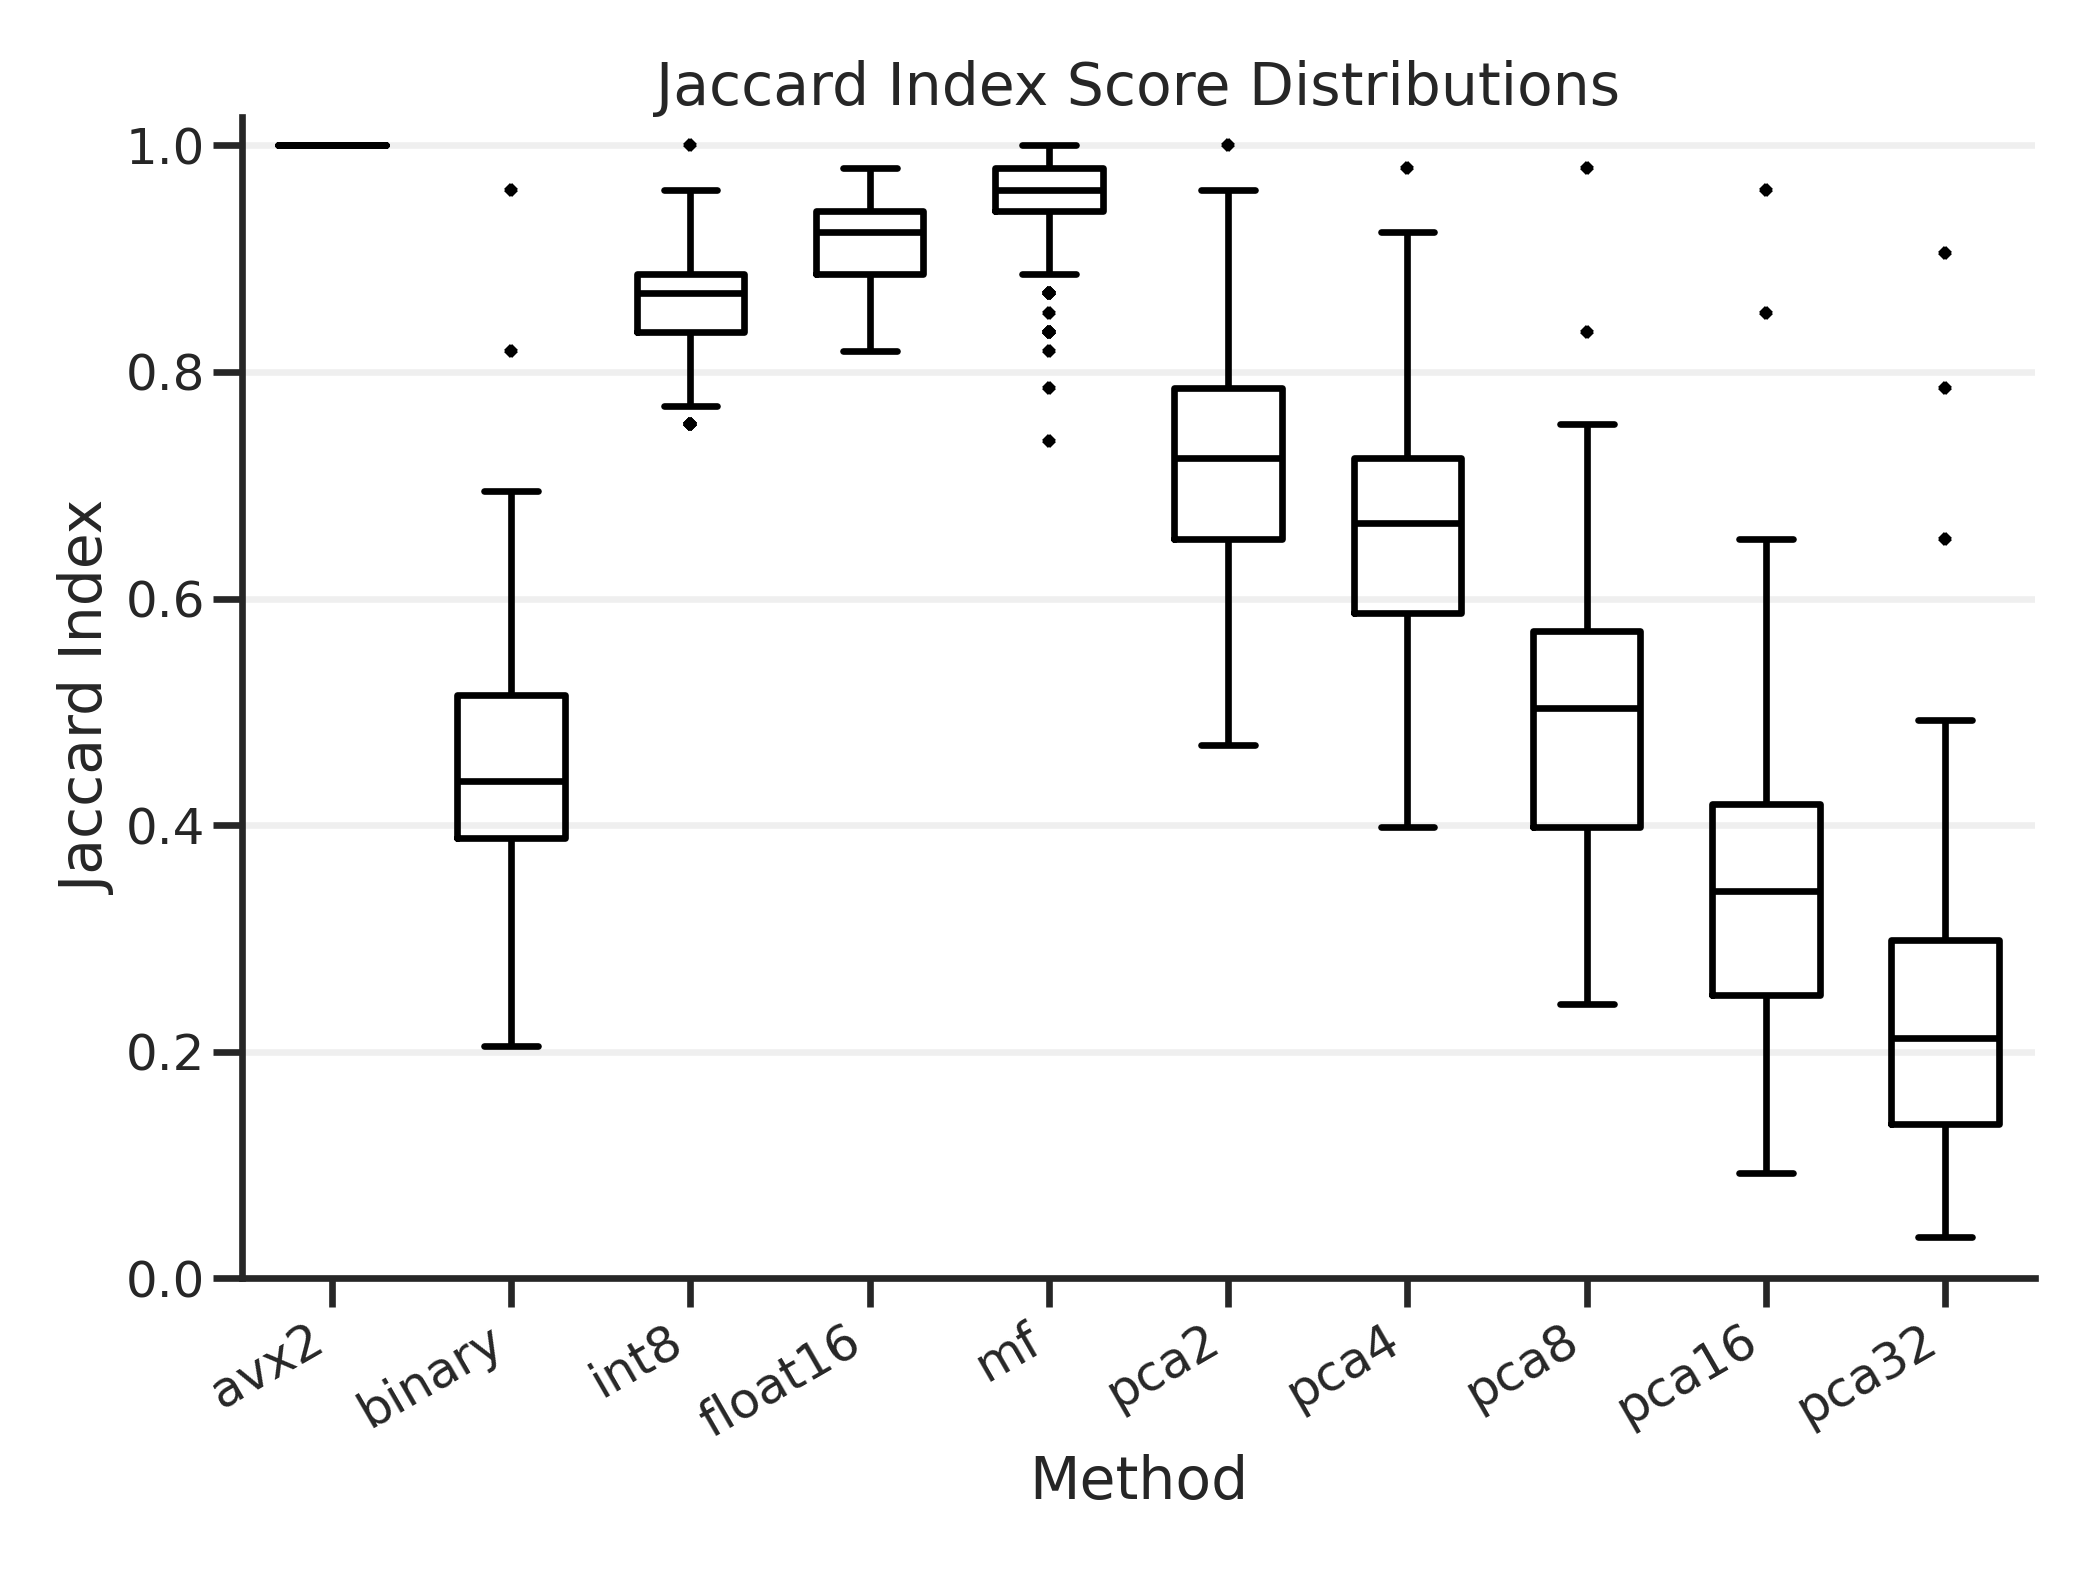
\includegraphics[width=0.49\widefigwidth]{bilder/plots/jaccard_boxplots_dim1024_k100_re.png}
      \vspace*{-1cm}
      \caption{Jaccard index of searchers with randomly generated queries}
      \label{boxjaccardsearchersone-re}
    \end{minipage}
    %\hfill
    \begin{minipage}{0.49\widefigwidth}
      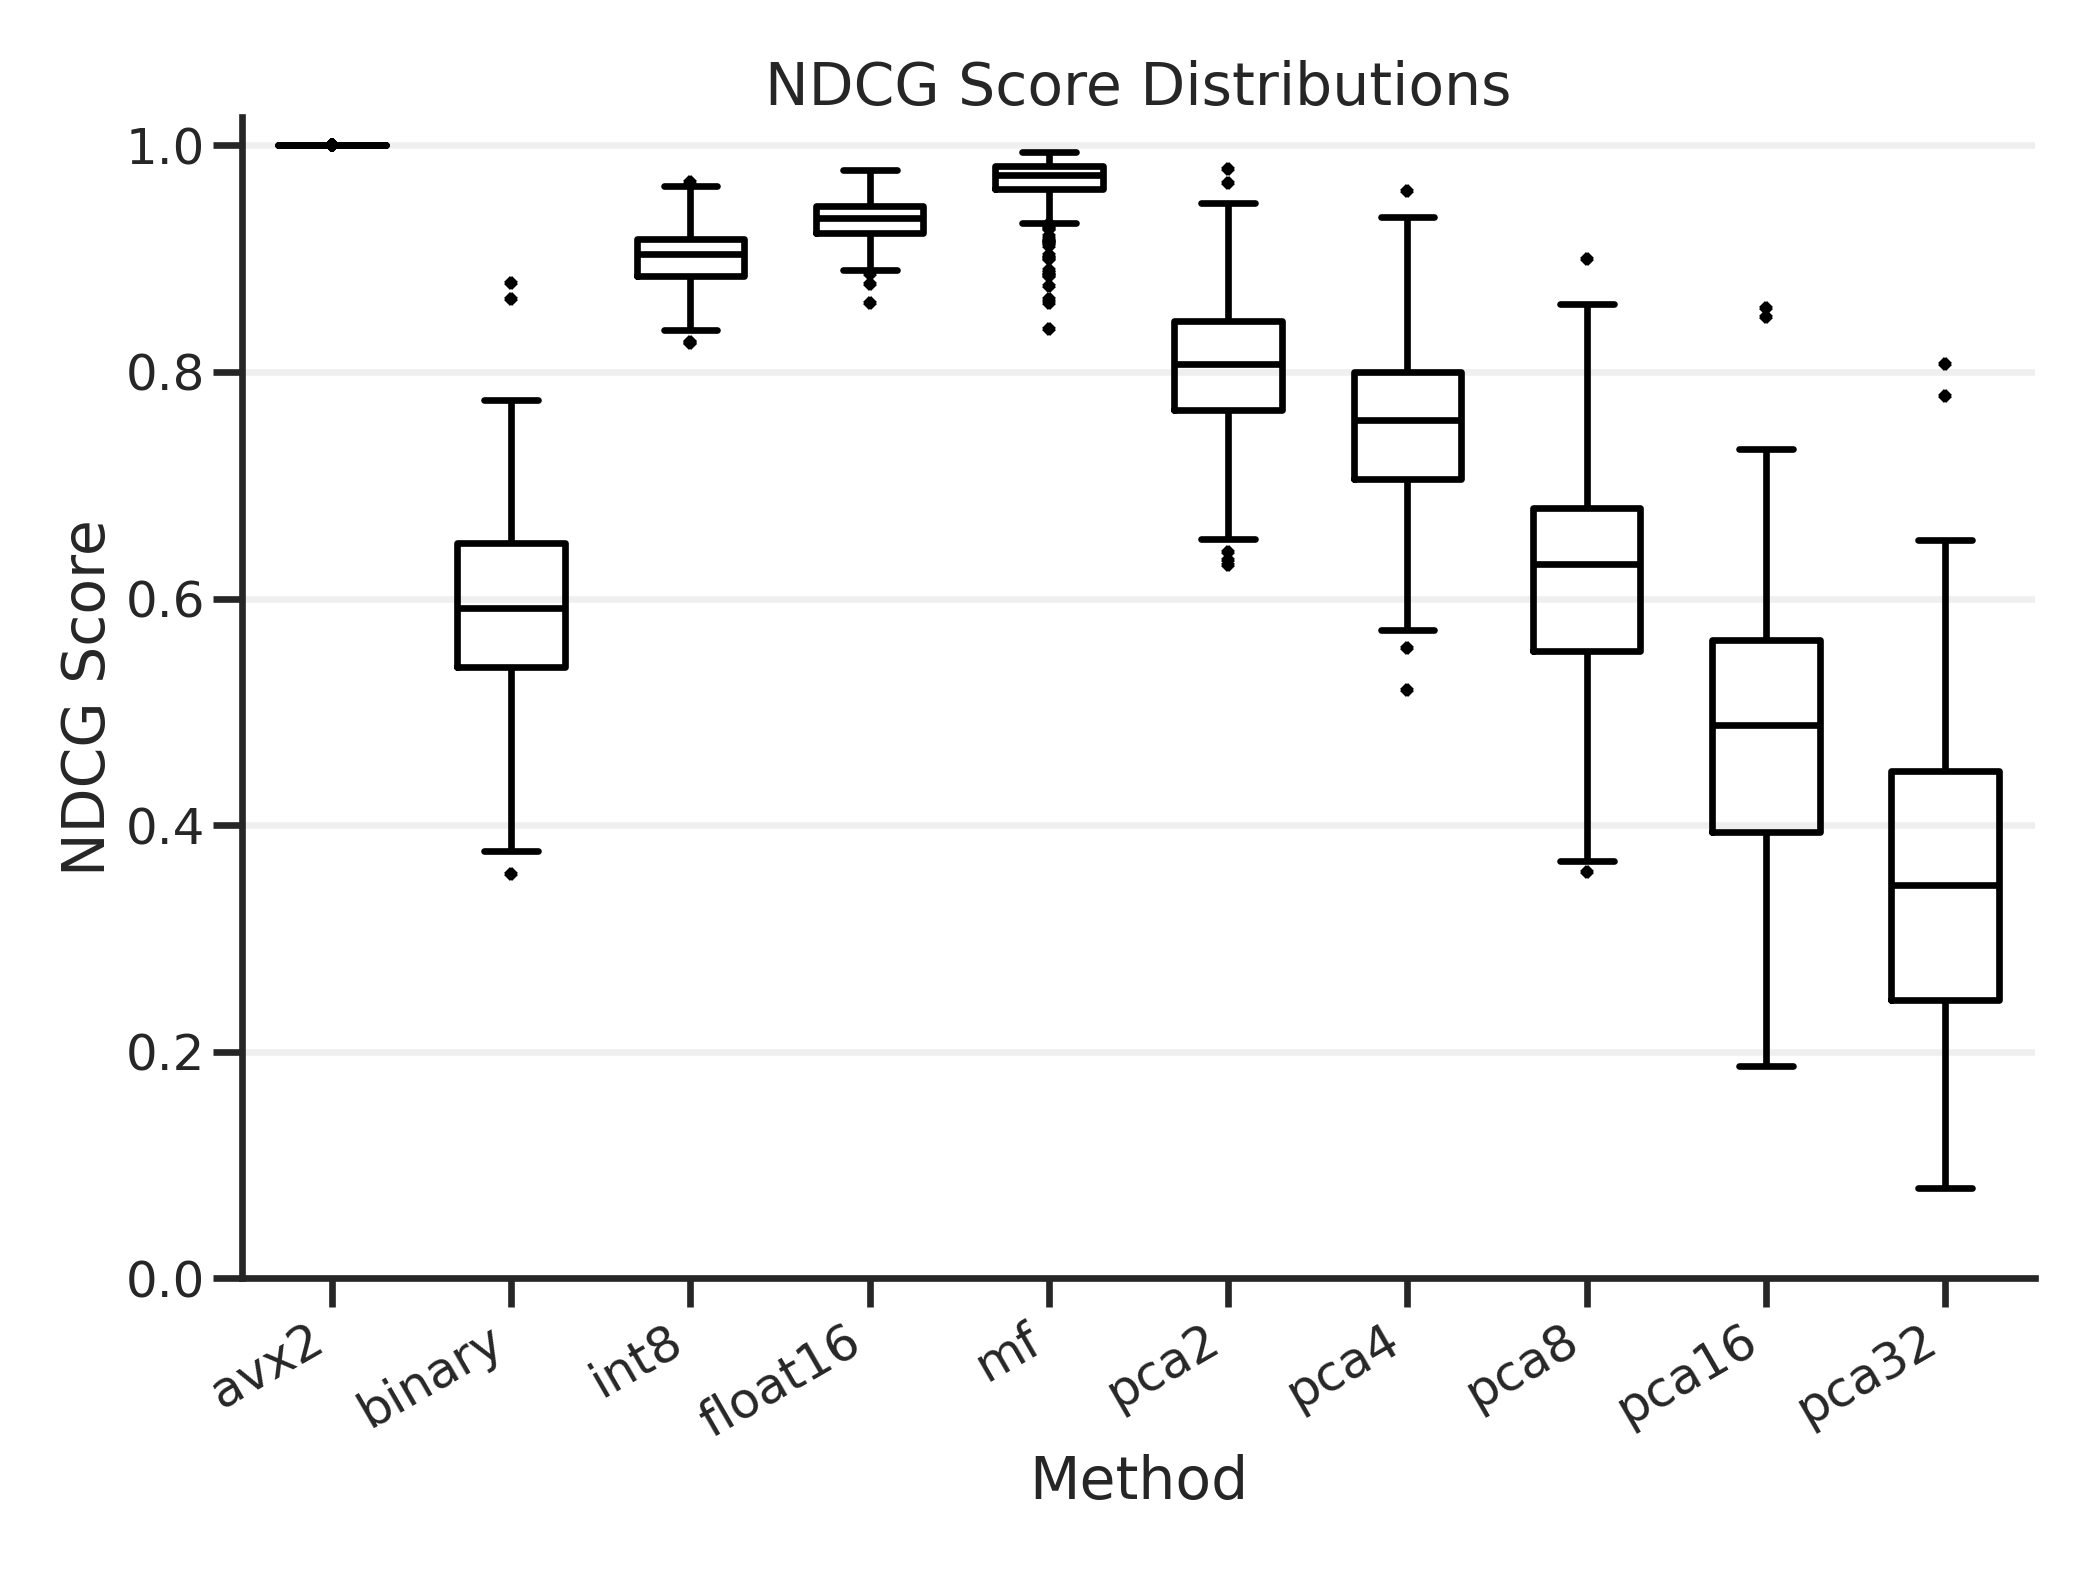
\includegraphics[width=0.49\widefigwidth]{bilder/plots/ndcg_boxplots_dim1024_k100_re.png}
      \vspace*{-1cm}
      \caption{NDCG score of searchers with randomly generated queries}
      \label{boxndcgsearchersone-re}
    \end{minipage}
  }
\end{figure}
\begin{figure}[h]
  \makebox[\textwidth][c]{%
    \begin{minipage}{0.49\widefigwidth}
      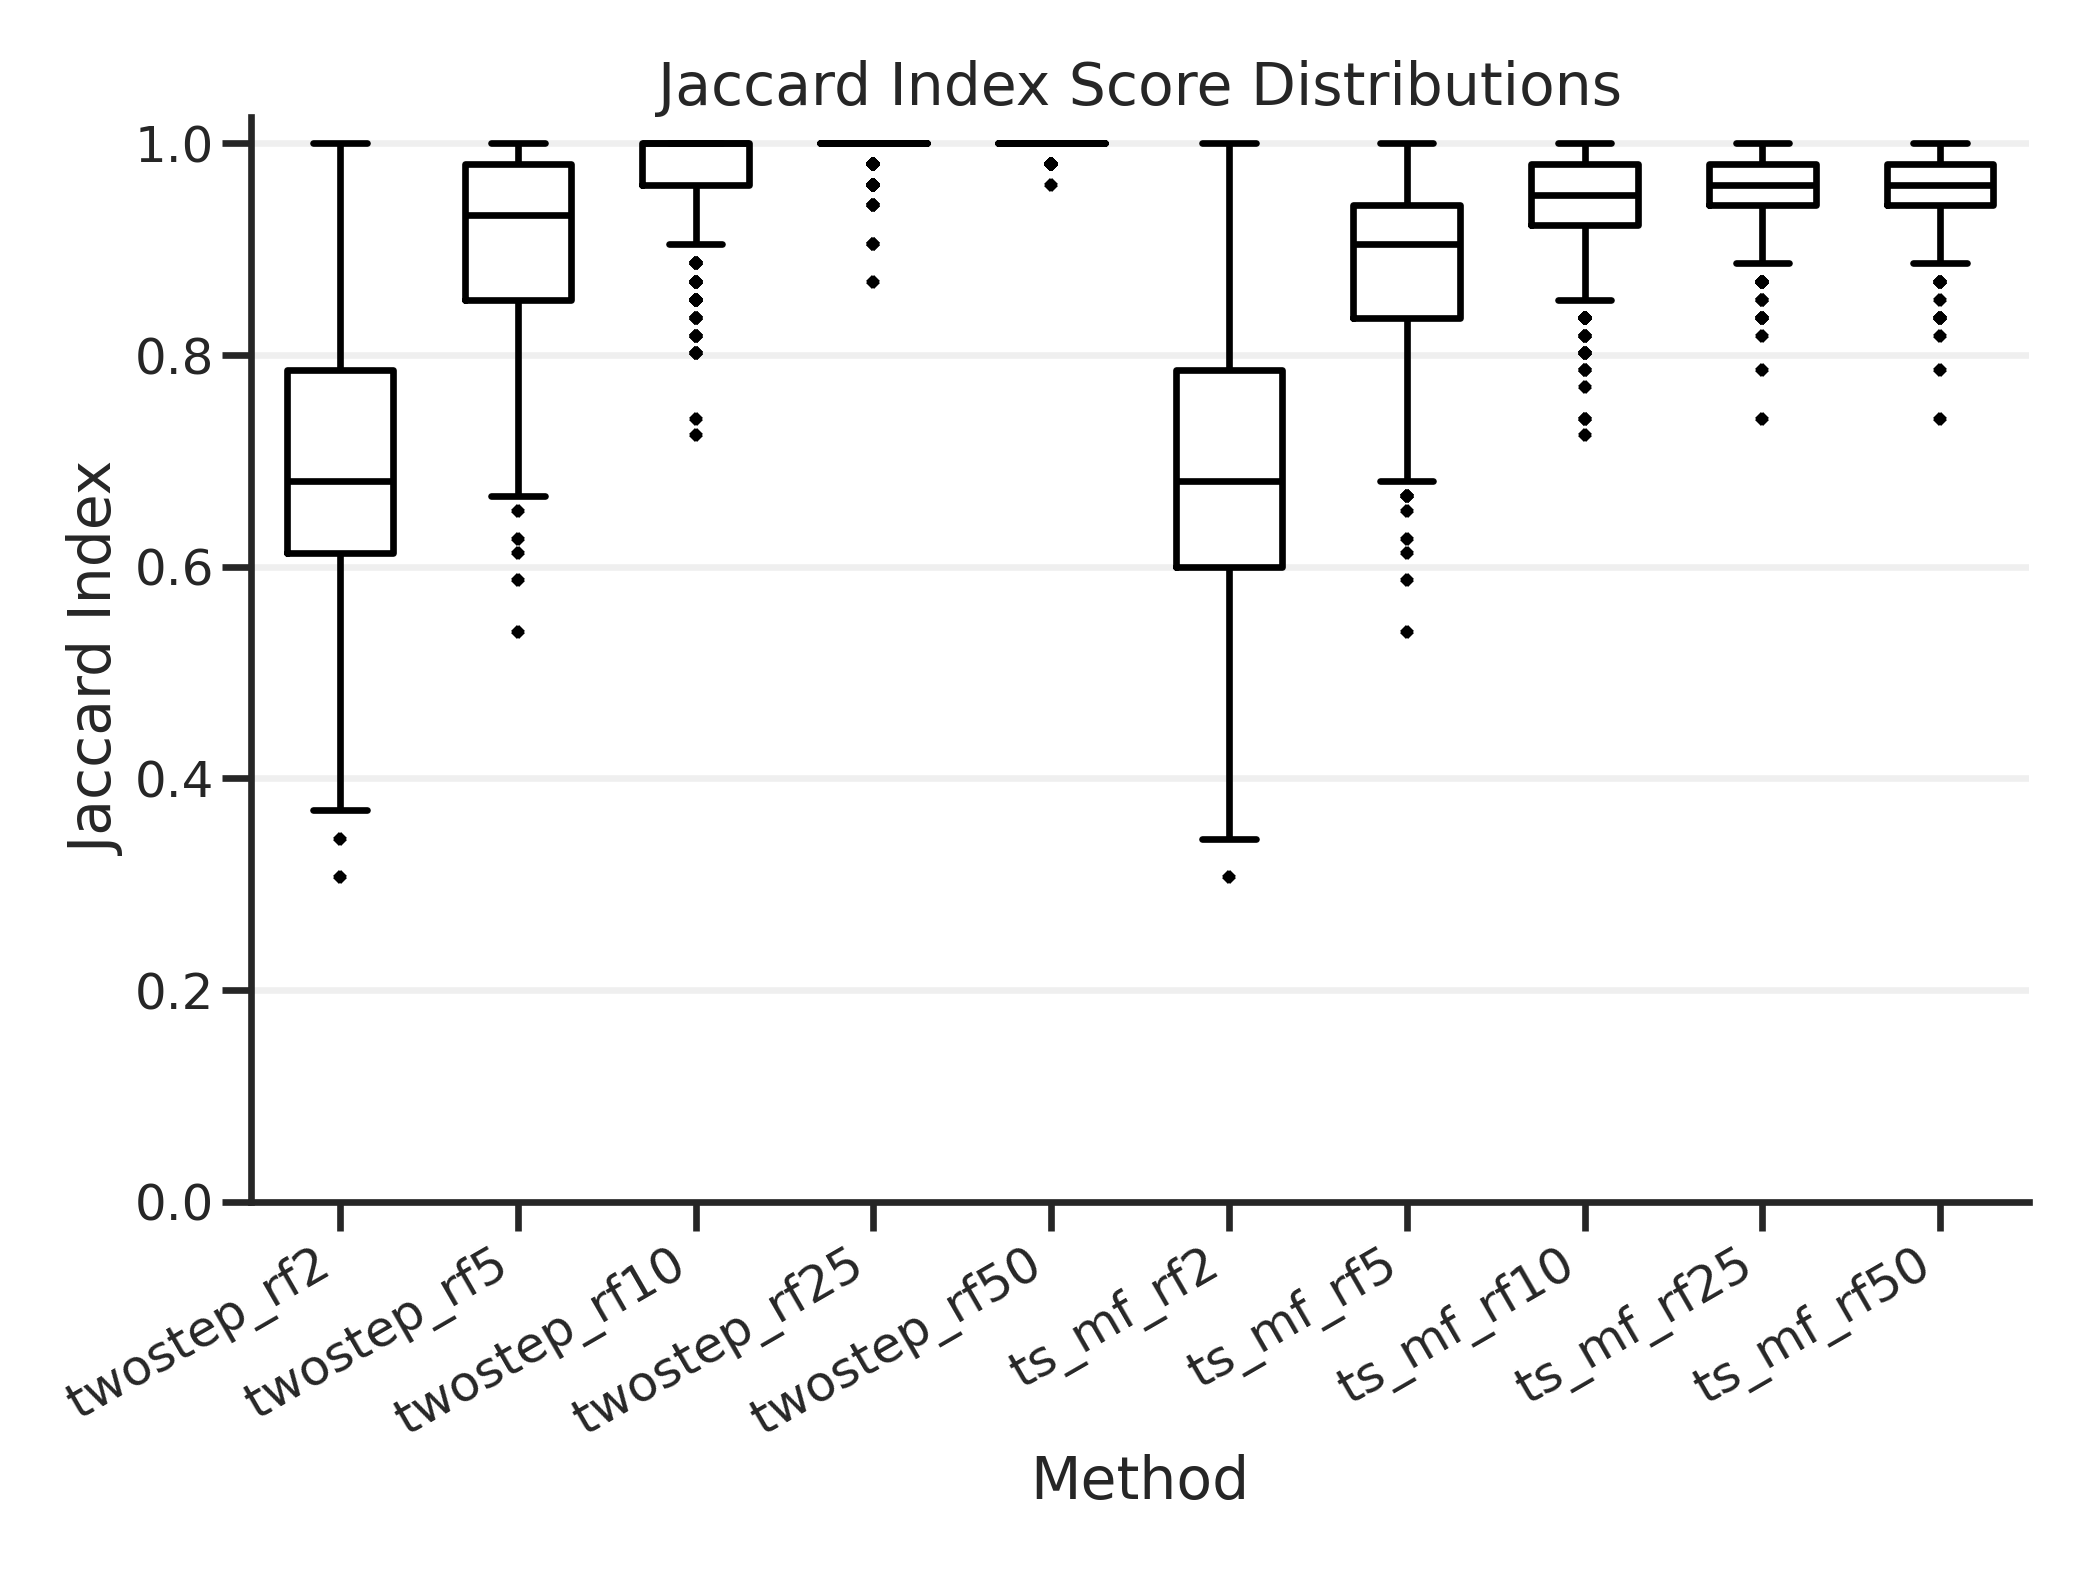
\includegraphics[width=0.49\widefigwidth]{bilder/plots/jaccard_boxplots_dim1024_k100_re_twostep.png}
      \vspace*{-1cm}
      \caption{Jaccard index of two-step searchers with randomly generated queries}
      \label{boxjaccardsearcherstwo-re}
    \end{minipage}
    %\hfill
    \begin{minipage}{0.49\widefigwidth}
      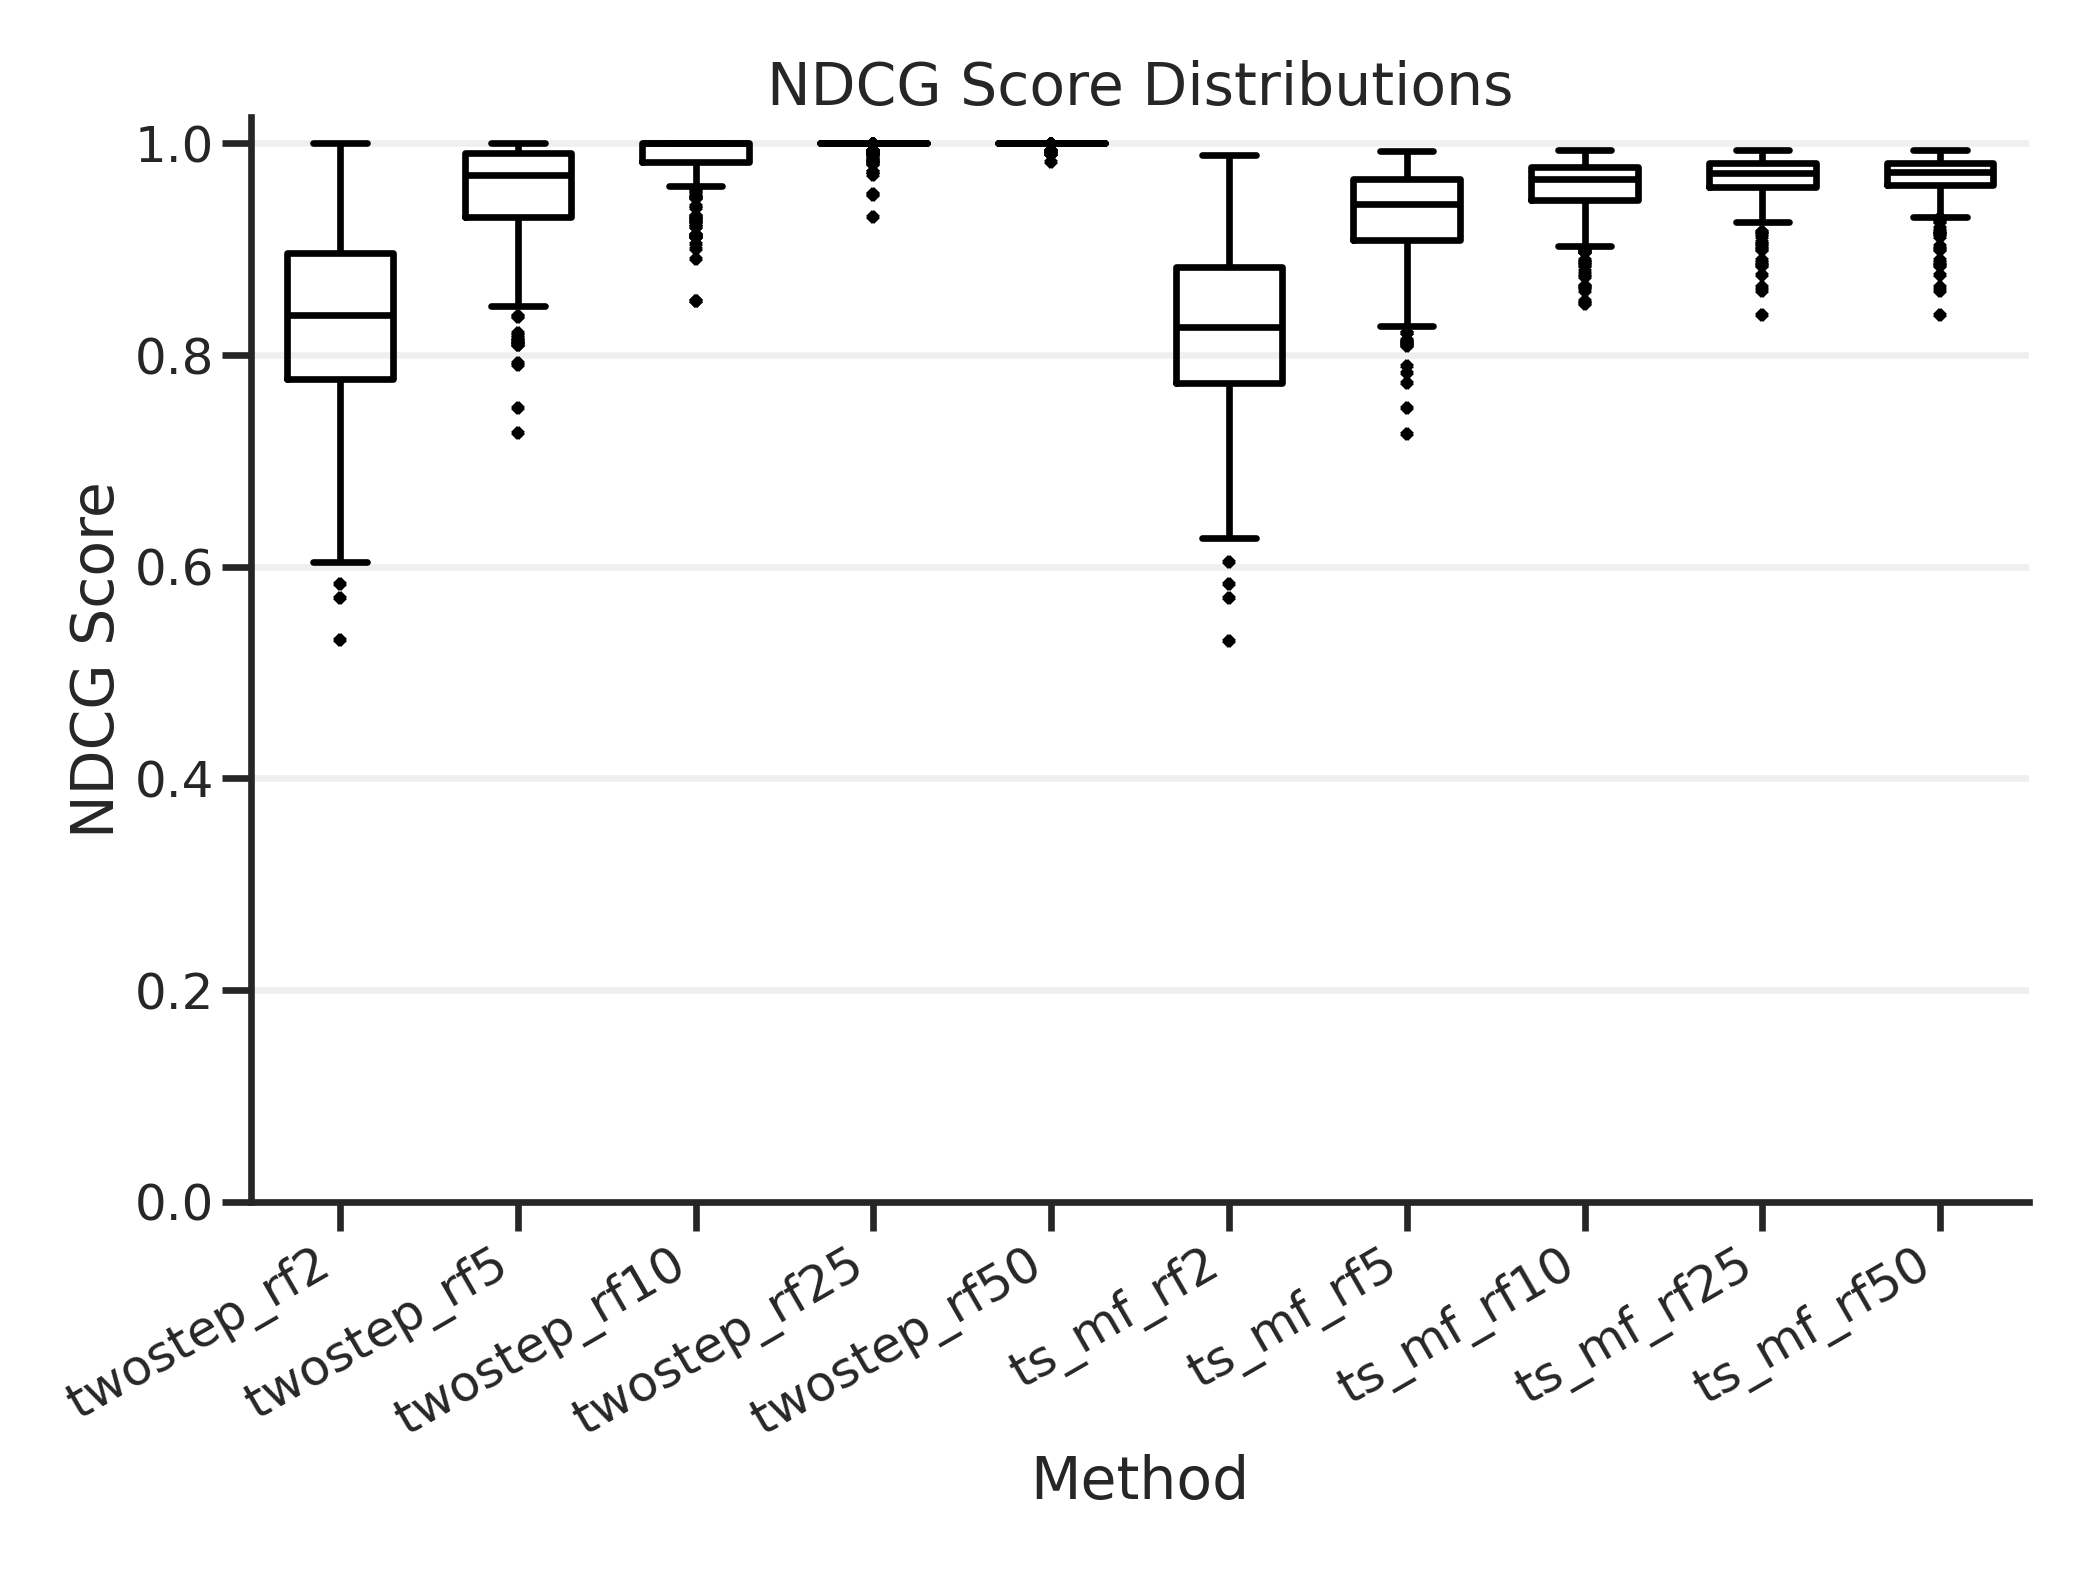
\includegraphics[width=0.49\widefigwidth]{bilder/plots/ndcg_boxplots_dim1024_k100_re_twostep.png}
      \vspace*{-1cm}
      \caption{NDCG score of two-step searchers with randomly generated queries}
      \label{boxndcgsearcherstwo-re}
    \end{minipage}
  }
\end{figure}
Looking at \autoref{boxjaccardsearchersone-re} \ref{boxndcgsearchersone-re} \ref{boxjaccardsearcherstwo-re} \ref{boxndcgsearcherstwo-re}: The searchers perform worse in accuracy across the board. But this isn't a drawback as this is not a realistic use case for embedding search.

\begin{table}[h]
  \centering
  \begin{tabular}{lccccccc}
    \hline
    Method       & Mean (ms) & Std Time & NDCG  & Jaccard & Overlap & M (GB) & BW (GB/s) \\
    \hline
    float        & 1105.232  & 0.948    & 1.000 & 1.000   & 100.000 & 4.578  & 4.142     \\
    avx2         & 135.972   & 1.105    & 1.000 & 1.000   & 100.000 & 4.578  & 33.666    \\
    binary       & 6.662     & 0.048    & 0.589 & 0.451   & 61.496  & 0.143  & 21.474    \\
    int8         & 95.215    & 0.055    & 0.901 & 0.867   & 92.836  & 1.144  & 12.019    \\
    float16      & 185.023   & 6.713    & 0.934 & 0.914   & 95.500  & 2.289  & 12.370    \\
    mf           & 540.883   & 0.325    & 0.966 & 0.956   & 97.692  & 1.144  & 2.116     \\
    pca2         & 71.421    & 0.607    & 0.803 & 0.724   & 83.700  & 2.291  & 32.047    \\
    pca4         & 38.725    & 0.314    & 0.750 & 0.653   & 78.544  & 1.145  & 29.552    \\
    pca8         & 22.146    & 0.217    & 0.616 & 0.489   & 64.820  & 0.573  & 25.838    \\
    pca16        & 12.469    & 0.201    & 0.482 & 0.346   & 50.140  & 0.286  & 22.944    \\
    pca32        & 7.566     & 0.129    & 0.351 & 0.228   & 35.720  & 0.143  & 18.908    \\
    twos\_rf2    & 6.583     & 0.065    & 0.830 & 0.689   & 80.772  & 4.721  & 21.846    \\
    twos\_rf5    & 6.727     & 0.063    & 0.952 & 0.904   & 94.660  & 4.721  & 21.550    \\
    twos\_rf10   & 7.006     & 0.067    & 0.985 & 0.969   & 98.344  & 4.721  & 20.963    \\
    twos\_rf25   & 7.952     & 0.089    & 0.998 & 0.995   & 99.748  & 4.721  & 19.188    \\
    twos\_rf50   & 9.486     & 0.124    & 1.000 & 0.999   & 99.948  & 4.721  & 17.091    \\
    ts\_mf\_rf2  & 6.600     & 0.054    & 0.821 & 0.684   & 80.452  & 1.287  & 21.702    \\
    ts\_mf\_rf5  & 6.930     & 0.053    & 0.930 & 0.880   & 93.384  & 1.287  & 20.711    \\
    ts\_mf\_rf10 & 7.476     & 0.062    & 0.956 & 0.934   & 96.516  & 1.287  & 19.262    \\
    ts\_mf\_rf25 & 9.131     & 0.086    & 0.965 & 0.953   & 97.548  & 1.287  & 15.927    \\
    ts\_mf\_rf50 & 11.820    & 0.136    & 0.966 & 0.955   & 97.668  & 1.287  & 12.506    \\
    \hline
  \end{tabular}
  \caption{Comparison of methods for mixedbread-ai/mxbai-embed-large-v1}
  \label{tab:method-comparison-1024}
\end{table}

\begin{table}[h]
  \centering
  \begin{tabular}{lccccccc}
    \hline
    Method       & Mean (ms) & Std Time & NDCG  & Jaccard & Overlap & M (GB) & BW (GB/s) \\
    \hline
    float        & 862.587   & 0.625    & 1.000 & 1.000   & 100.000 & 3.433  & 3.980     \\
    avx2         & 91.731    & 1.469    & 1.000 & 1.000   & 100.000 & 3.433  & 37.427    \\
    binary       & 9.022     & 0.063    & 0.605 & 0.475   & 63.664  & 0.107  & 11.891    \\
    int8         & 72.253    & 0.094    & 0.930 & 0.910   & 95.248  & 0.858  & 11.879    \\
    float16      & 142.844   & 18.197   & 0.967 & 0.959   & 97.880  & 1.717  & 12.017    \\
    mf           & 408.601   & 0.357    & 0.992 & 0.989   & 99.468  & 0.858  & 2.101     \\
    pca2         & 51.656    & 0.481    & 0.901 & 0.864   & 92.624  & 1.718  & 33.231    \\
    pca4         & 29.478    & 0.331    & 0.820 & 0.754   & 85.648  & 0.859  & 29.117    \\
    pca8         & 16.082    & 0.156    & 0.626 & 0.505   & 66.076  & 0.429  & 26.685    \\
    pca16        & 9.487     & 0.141    & 0.441 & 0.309   & 45.680  & 0.215  & 22.618    \\
    pca32        & 5.767     & 0.112    & 0.285 & 0.174   & 28.260  & 0.107  & 18.602    \\
    twos\_rf2    & 9.076     & 0.031    & 0.848 & 0.717   & 82.772  & 3.541  & 11.884    \\
    twos\_rf5    & 9.241     & 0.031    & 0.962 & 0.924   & 95.828  & 3.541  & 11.764    \\
    twos\_rf10   & 9.521     & 0.034    & 0.991 & 0.981   & 99.008  & 3.541  & 11.569    \\
    twos\_rf25   & 10.404    & 0.060    & 0.999 & 0.998   & 99.900  & 3.541  & 11.000    \\
    twos\_rf50   & 11.816    & 0.101    & 1.000 & 1.000   & 99.976  & 3.541  & 10.291    \\
    ts\_mf\_rf2  & 9.157     & 0.065    & 0.847 & 0.717   & 82.760  & 0.966  & 11.732    \\
    ts\_mf\_rf5  & 9.465     & 0.024    & 0.959 & 0.921   & 95.684  & 0.966  & 11.373    \\
    ts\_mf\_rf10 & 9.965     & 0.034    & 0.985 & 0.974   & 98.632  & 0.966  & 10.839    \\
    ts\_mf\_rf25 & 11.479    & 0.063    & 0.991 & 0.988   & 99.384  & 0.966  & 9.502     \\
    ts\_mf\_rf50 & 13.903    & 0.113    & 0.992 & 0.989   & 99.444  & 0.966  & 7.974     \\
    \hline
  \end{tabular}
  \caption{Comparison of methods for sentence-transformers/all-mpnet-base-v2}
  \label{tab:method-comparison-768}
\end{table}
% % Abbildungsverzeichnis
% \listoffigures
% \addcontentsline{toc}{chapter}{Abbildungsverzeichnis}
% \cleardoublepage
% % Algorithmenverzeichnis
% \listofalgorithms
% \addcontentsline{toc}{chapter}{Algorithmenverzeichnis}
% \cleardoublepage
% Literaturverzeichnis, is now mostly defined in the header
\printbibliography
\addcontentsline{toc}{chapter}{\bibname}
% Erklaerung
% \markboth{}{ERKLÄRUNG}
\addcontentsline{toc}{chapter}{Affidavit}
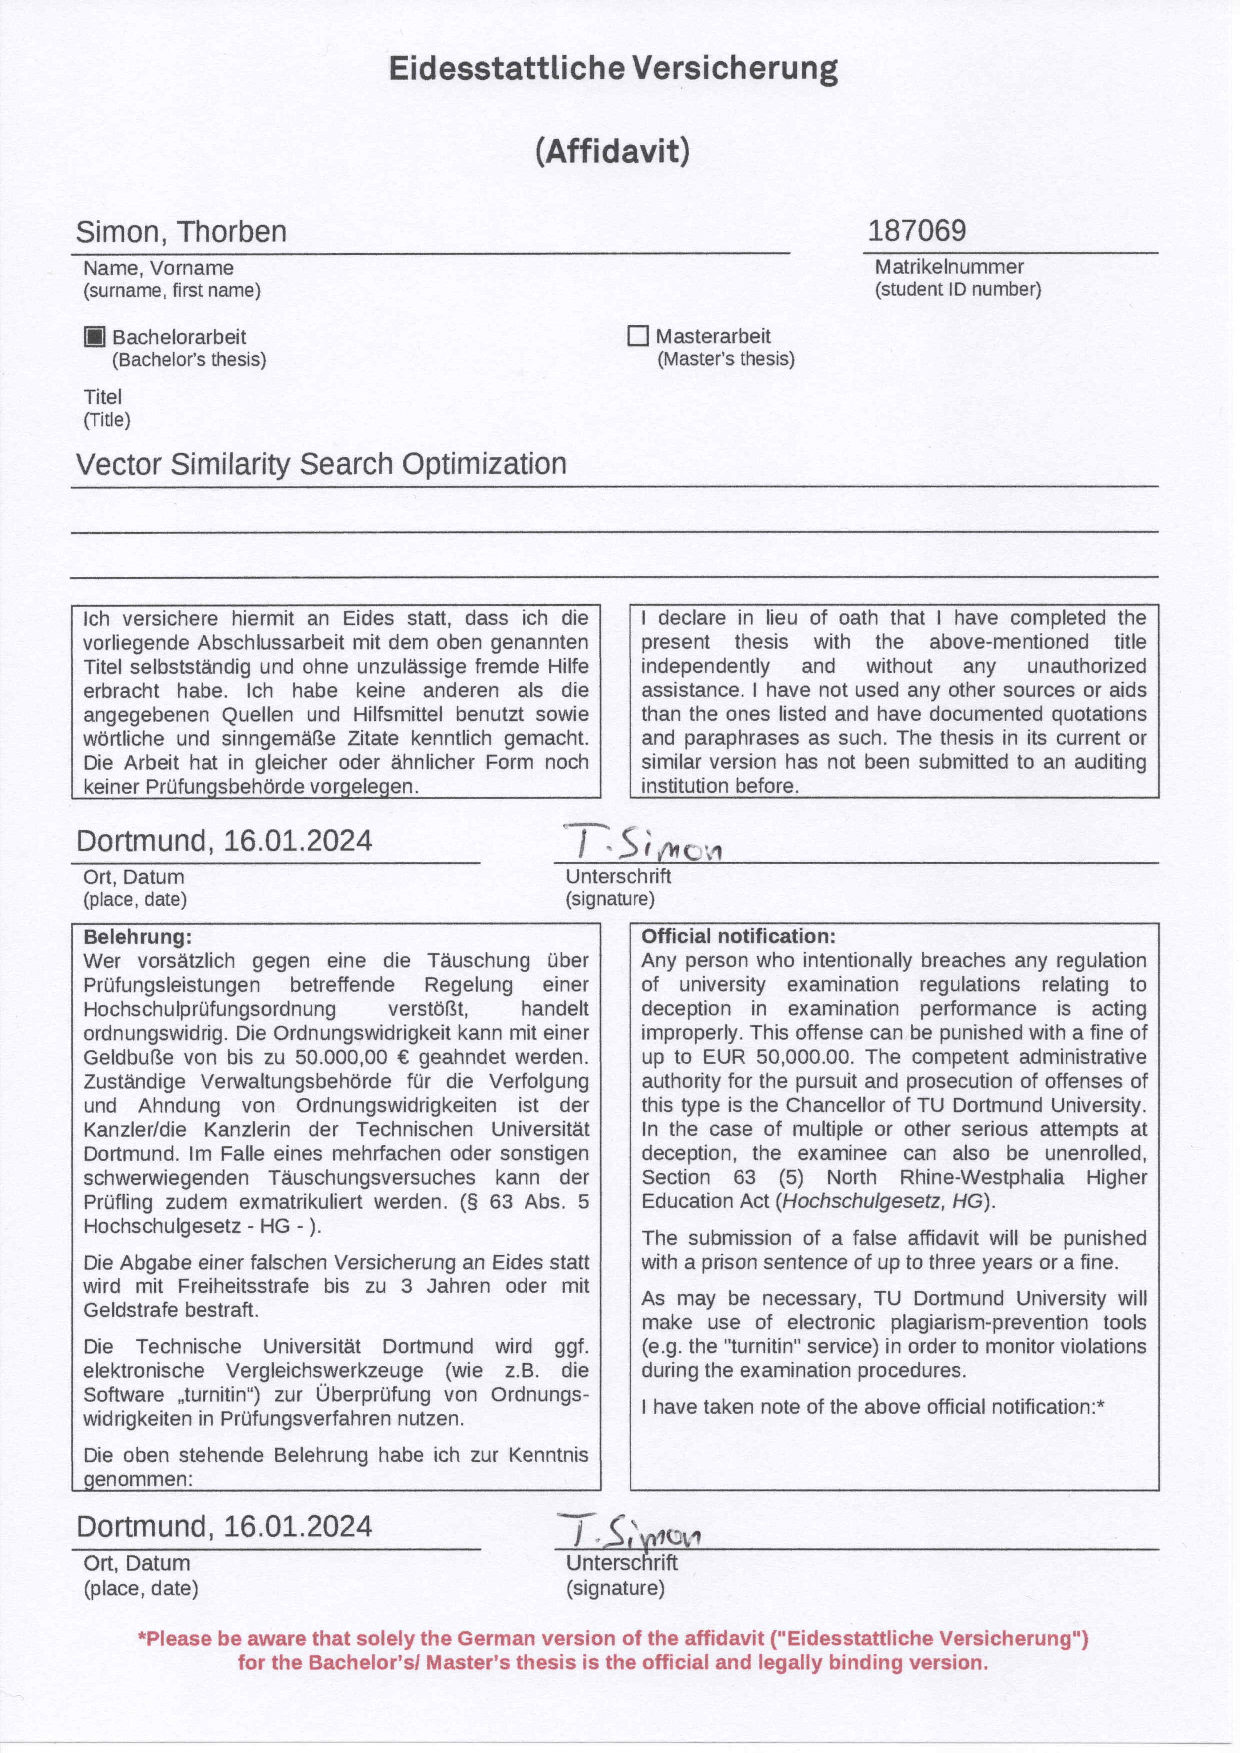
\includepdf[pages=-]{kapitel/Eidesstattliche_Versicherung_signed.pdf}
% % erklaerung.tex
\cleardoublepage
\normalsize
Hiermit versichere ich, dass ich die vorliegende Arbeit selbstständig verfasst habe und keine anderen als die angegebenen Quellen und Hilfsmittel verwendet sowie Zitate kenntlich gemacht habe.\\\\
Dortmund, den \today \\\\\\\\
Muster Mustermann
% EOF
% \cleardoublepage
\end{document}

